% !TeX program = xelatex
% XeLaTeX is recommended; pdfLaTeX and LuaLaTeX are supported too.
\documentclass[11pt,a4paper,oneside]{report}
\usepackage[left=25mm,right=23mm,top=23mm,bottom=24mm,headheight=15pt]{geometry}
\usepackage{iftex}
\ifPDFTeX
  % Type 1 editions of the same font families work with pdfLaTeX.
  \usepackage[T1]{fontenc}
  \usepackage[utf8]{inputenc}
  \usepackage{tgpagella,tgheros}
  \usepackage[scale=0.88]{tgcursor}
\else
  % OpenType font configuration for XeLaTeX, LuaLaTeX and Tectonic.
  \usepackage{fontspec}
  \setmainfont{texgyrepagella-regular.otf}[BoldFont=texgyrepagella-bold.otf,ItalicFont=texgyrepagella-italic.otf,BoldItalicFont=texgyrepagella-bolditalic.otf]
  \setsansfont{texgyreheros-regular.otf}[BoldFont=texgyreheros-bold.otf,ItalicFont=texgyreheros-italic.otf]
  \setmonofont{texgyrecursor-regular.otf}[BoldFont=texgyrecursor-bold.otf,ItalicFont=texgyrecursor-italic.otf,BoldItalicFont=texgyrecursor-bolditalic.otf,Scale=0.88]
\fi
\usepackage{amsmath,amssymb,booktabs,longtable,tabularx,array,graphicx,xcolor}
\usepackage{fancyhdr,titlesec,enumitem,listings,needspace,etoolbox,xurl,ragged2e}
\usepackage[protrusion=true,expansion=false]{microtype}
\usepackage[unicode,colorlinks=true,linkcolor=navy,urlcolor=teal,citecolor=navy]{hyperref}
\definecolor{navy}{HTML}{17324D}
\definecolor{teal}{HTML}{277D77}
\definecolor{muted}{HTML}{526371}
\definecolor{wash}{HTML}{F1F4F7}
\definecolor{rulegray}{HTML}{D2DCE3}
\hypersetup{pdftitle={SafeSliceSQL: Complete Project Workflow and Review Guide},pdfauthor={Prepared from the SafeSliceSQL repository},pdfsubject={Plain-language and technical walkthrough, file atlas, functions, parameters and measured evidence},bookmarksnumbered=true}
\AtBeginDocument{\RaggedRight}
\setlength{\parindent}{0pt}
\setlength{\parskip}{6pt}
\linespread{1.10}
\setlength{\emergencystretch}{3em}
\setlength{\tabcolsep}{3pt}
\renewcommand{\arraystretch}{1.15}
\AtBeginEnvironment{longtable}{\small}
\setlist[itemize]{leftmargin=1.5em,itemsep=3pt,topsep=4pt}
\setlist[enumerate]{leftmargin=1.8em,itemsep=4pt,topsep=4pt}
\titleformat{\chapter}[display]{\sffamily\bfseries\color{navy}}{\large\chaptertitlename\ \thechapter}{5pt}{\LARGE}
\titlespacing*{\chapter}{0pt}{0pt}{16pt}
\titleformat{\section}{\sffamily\large\bfseries\color{navy}}{\thesection}{0.6em}{}
\titleformat{\subsection}{\sffamily\normalsize\bfseries\color{navy}}{\thesubsection}{0.6em}{}
\titlespacing*{\section}{0pt}{14pt}{5pt}
\titlespacing*{\subsection}{0pt}{10pt}{3pt}
\pagestyle{fancy}
\fancyhf{}
\fancyhead[L]{\sffamily\small\color{muted}SafeSliceSQL | Project workflow and review guide}
\fancyfoot[L]{\sffamily\footnotesize\color{muted}Source snapshot: 25 November 2026}
\fancyfoot[R]{\sffamily\small\thepage}
\renewcommand{\headrulewidth}{0.3pt}
\renewcommand{\footrulewidth}{0pt}
\fancypagestyle{plain}{\fancyhf{}\fancyfoot[L]{\sffamily\footnotesize\color{muted}SafeSliceSQL | Reviewed 25 November 2026}\fancyfoot[R]{\sffamily\small\thepage}\renewcommand{\headrulewidth}{0pt}}
\lstset{basicstyle=\ttfamily\footnotesize,keywordstyle=\color{navy}\bfseries,commentstyle=\color{muted},stringstyle=\color{teal},backgroundcolor=\color{wash},frame=single,rulecolor=\color{rulegray},framerule=0.3pt,framesep=7pt,breaklines=true,breakatwhitespace=false,columns=fullflexible,keepspaces=true,showstringspaces=false,tabsize=4,aboveskip=8pt,belowskip=8pt}
\newcommand{\plain}[1]{\par\textbf{In plain language.} #1\par}
\newcommand{\technical}[1]{\par\textbf{Technically.} #1\par}
\newcommand{\source}[1]{\par{\small\color{muted}\textbf{Implementation:} \path{#1}}\par}
\newcommand{\reviewpoint}[1]{\par\begingroup\setlength{\fboxsep}{9pt}\noindent\colorbox{wash}{\parbox{\dimexpr\linewidth-18pt\relax}{\textbf{Review highlight.} #1}}\endgroup\par}
\setcounter{tocdepth}{1}
\setcounter{secnumdepth}{2}

\begin{document}
\hypersetup{pageanchor=false}
\begin{titlepage}
\thispagestyle{empty}
\vspace*{13mm}
{\sffamily\large\bfseries\color{teal}PROJECT UNDERSTANDING SERIES\par}
\vspace{13mm}
{\sffamily\fontsize{37}{43}\selectfont\bfseries\color{navy}SafeSliceSQL\par}
\vspace{6mm}
{\sffamily\fontsize{22}{28}\selectfont\color{navy}Complete Workflow\par and Project Review Guide\par}
\vspace{12mm}
{\Large From the first input to the committed copy,\par with a file-by-file explanation.\par}
\vspace{10mm}
\rule{\linewidth}{0.6pt}
\vspace{5mm}
\begin{tabularx}{\linewidth}{@{}>{\RaggedRight\arraybackslash}p{.25\linewidth}X@{}}
\textbf{Audience} & Student, evaluator, developer and future maintainer \\
\textbf{Reading style} & Plain-language explanations alongside technical detail \\
\textbf{Project version} & 0.1.0; Python 3.10+; MySQL 8.x / InnoDB application scope \\
\textbf{Reviewed} & 25 November 2026 \\
\textbf{Source baseline} & \path{ac58c45a8b7d34c948e39332f2ad157f241edbbc} \\
\end{tabularx}
\vfill
\reviewpoint{The central promise is a smaller, checked database under a hard total-row budget, with the required parent records preserved. Query preservation is measured and gated; it is not guaranteed merely by keeping foreign keys valid.}
\vspace{8mm}
{\small Prepared from local application source, configuration, tests and saved result artifacts. Private connection secrets are excluded. Fresh checks and historical measurements are labelled separately.\par}
\end{titlepage}

\hypersetup{pageanchor=true}
\pagenumbering{roman}
\chapter*{How to use this guide}
\addcontentsline{toc}{chapter}{How to use this guide}
This document answers four questions in order: \emph{What does the project do? How does one job actually run? Which file owns each behavior? What evidence can you show in a review?}

For a first reading, follow Chapters 1--8. They explain the workflow, inputs, algorithms, parameters, metrics and evidence. Chapter 9 gives a practical runbook; Chapter 10 prepares you for a review. The appendices are a lookup reference for every application module, supporting tracked file, test module and module/class function.

Each \textbf{In plain language} paragraph gives the idea without assuming database expertise. Each \textbf{Technically} paragraph connects it to the implementation. Code paths, defaults and formulas refer to the inspected source, not a hypothetical future design.

\textbf{Evidence labels matter.} ``Fresh'' means a check was run while preparing this guide. ``Saved'' or ``historical'' means the result was read from an existing local artifact. ``Example'' means an explanatory calculation, not a benchmark observation. The three labels are never interchangeable.

\textbf{What ``Fn values'' means here.} The guide includes function signatures, inputs, return objects, default values and scoring constants. The software is not a classifier, so it does not report a classification confusion matrix, false-negative count or F1 score. Its reported metrics concern database integrity, query survival, result retention and runtime.

\textbf{Coverage boundary.} The atlas covers all 103 tracked repository files in the reviewed snapshot, including 45 application Python modules and 28 behavioral test modules. Generated folders and third-party payloads are explained by their purpose and provenance. The source inventory records SHA-256 hashes; the evidence snapshot records the specific results cited here.

\tableofcontents
\clearpage
\pagenumbering{arabic}

\chapter{The project in one clear picture}
\section{The problem being solved}
\plain{A large database is inconvenient when you only need a small copy for development, testing or a demonstration. Picking records independently can leave an order without its customer, or a salary without its employee. SafeSliceSQL chooses a smaller set and includes the records those choices depend on.}
\technical{SafeSliceSQL is a Python database-subsetting application. Given a source schema, a fixed read-only SQL workload, a row budget and a random seed, it selects row keys, computes required foreign-key parent closure, materializes a separate target and measures query behavior. A heuristic chooses the subset; validation and acceptance decide whether it can be committed.}

The copy is stored in MySQL for the supported desktop/CSV application flow. SQLite is also used for local tests, example benchmarks and the temporary query-result comparison store. Supporting SQLite internally does not mean that PostgreSQL, SQL Server or arbitrary SQLAlchemy backends are part of the supported application promise.

\section{What is the main file?}
There are several entry points, each with a different responsibility:
\begin{itemize}
\item \path{demo.bat} starts the desktop presentation. \path{desktop.py:main()} starts Tkinter; the \path{Desktop} class owns the window.
\item \path{cli.py:app} is the Typer command-line application installed as \path{safeslice}. \path{Terminal Demo.bat} opens the numbered menu in \path{demo.py}.
\item \path{desktop_service.py:create_copy()} turns a desktop request into prepared input and benchmark settings.
\item \textbf{\path{pipeline.py:run_pipeline()}} is the core coordinator for one checked slice. It calls the selector, materializer, workload evaluator, structural validator and acceptance gate.
\item \path{sampler.py:select_rows()} owns the three selection strategies. It is the main algorithm file, but does not itself commit a database copy.
\end{itemize}
\reviewpoint{If an evaluator asks for ``the main algorithm'', show \path{sampler.py} with \path{dependency_graph.py}. If asked for ``the complete execution'', show \path{pipeline.py}. If asked for ``what starts the app'', show the launcher and \path{desktop.py}/\path{cli.py}.}

\section{One-page execution map}
\begin{figure}[htbp]
\centering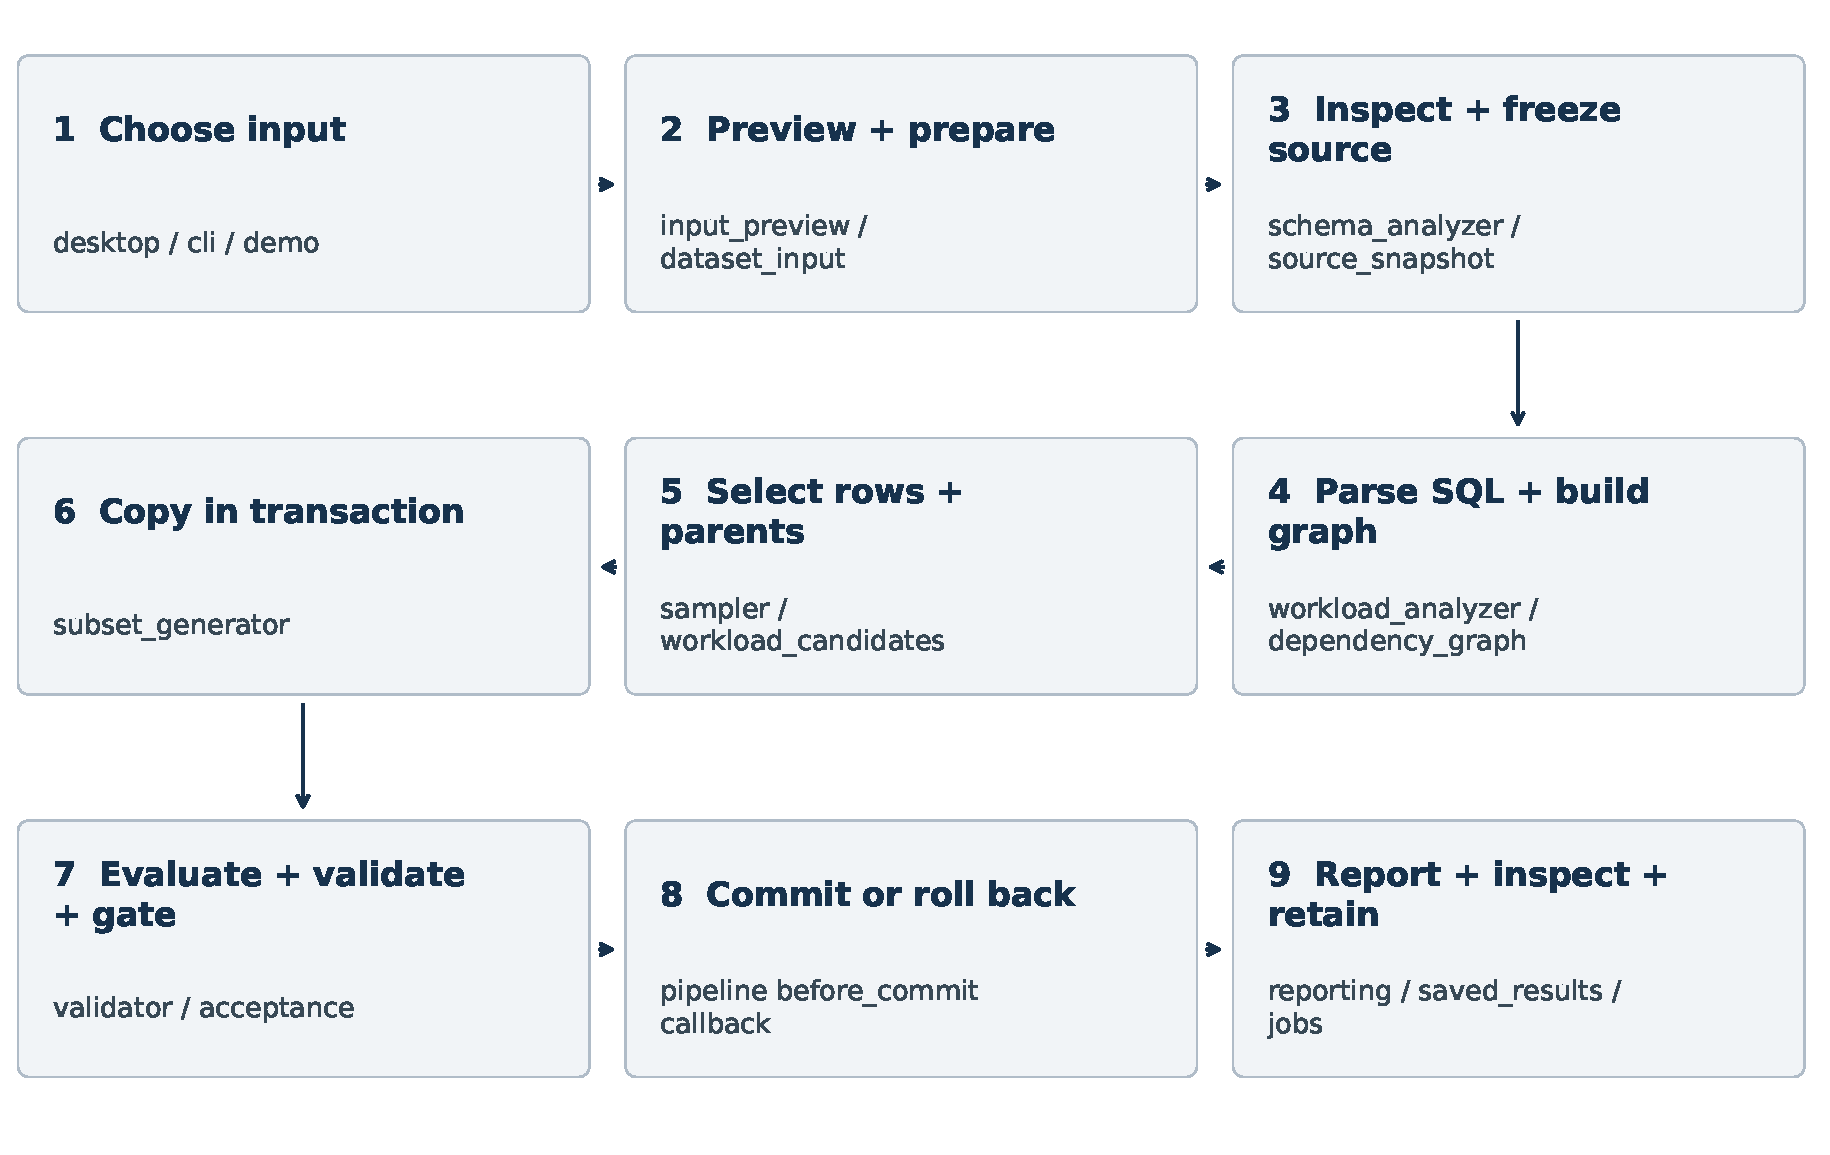
\includegraphics[width=\linewidth]{assets/workflow.pdf}
\caption{The common end-to-end flow. The target transaction remains open while the callback evaluates workload, validates the subset and applies the quality gate. Source: current application code.}
\end{figure}

\section{The four objects you should keep separate}
\begin{description}[style=nextline,leftmargin=1.5em,labelindent=0pt]
\item[Source database] The original relational input. Existing user-selected sources are read through read-only connections. CSV/Excel input first becomes a newly owned imported source schema.
\item[Target database] The separate smaller copy. Desktop jobs create a fresh UUID-named target; the CLI can refresh an explicitly named compatible target.
\item[Workload] A file of supported SELECT statements describing query behavior worth checking. The app can generate structural queries, but these are not automatically your real business requirements.
\item[Report artifacts] CSV/JSON/YAML/HTML/PNG files describing what was attempted, selected, committed, measured or rejected. A report directory is not an SQL database dump.
\end{description}

\chapter{A job from the first click to the final output}
\section{Start, load settings and show the interface}
\plain{The launcher opens the app using the project's Python environment. You choose data and a copy percentage. The program reads where your MySQL servers are, but connection passwords do not belong in reports.}
\technical{The batch launcher sets the project working directory and PYTHONPATH. Configuration loads the project-relative environment file into separate source and target DatabaseConfig objects, represented by SQLAlchemy URLs. Desktop defaults are a 10-percent budget, workload-aware selection, seed 42, minimum survival 1.0 and minimum exact retention 0.0. CLI run requires method and percentage explicitly and defaults its quality thresholds to 0.0 for compatibility.}
\source{demo.bat; src/safeslicesql/config.py; src/safeslicesql/desktop_service.py; src/safeslicesql/cli.py}

\section{Preview without creating a copy}
\plain{The preview tells you the input's size so you can choose a sensible limit. It also warns when a schema or file cannot be handled.}
\technical{\path{preview_input()} streams files with \path{iter_input_tables()}, or inspects an existing database using a read-only source engine. It validates row widths and configured limits. MySQL table counts are exact COUNT-based counts rather than information-schema estimates. The current CLI inspection label still says ``approx'', but the underlying counts are exact. No target is constructed for a CLI --dry-run selection.}
\source{src/safeslicesql/input_preview.py; src/safeslicesql/schema_analyzer.py; src/safeslicesql/cli.py}

\section{Prepare one of two input paths}
\subsection{Path A: existing MySQL database}
Select a database already imported into MySQL. SafeSliceSQL reads its declared types and keys, generates a structural workload and creates a separate target schema such as \path{safeslice_output_<16-hex-token>}. The application does not interpret a downloaded .sql dump through the CSV picker; load that dump with a MySQL client first.
\subsection{Path B: CSV, CSV folder or XLSX workbook}
The app creates \path{safeslice_input_<token>} on the \emph{target server}, streams tables into it and adds integer \path{_safeslice_id} keys. It creates an additional output schema for the smaller copy. Files are therefore not processed entirely without MySQL, even though previewing a CSV can happen without a server.

Table names follow \path{data_<number>_<sanitized-file-or-sheet-stem>}. CSV cells are preserved as strings in text/LONGTEXT columns; empty CSV fields remain empty strings. Excel None cells can become SQL NULL, and formulas are read as formula text. Header normalization resolves blanks, duplicate/case-equivalent names and the generated-key collision, retaining a mapping in the manifest. Types and relationships are not inferred.
\source{src/safeslicesql/dataset_input.py}

\section{Create the job record and experiment settings}
\plain{The app records the work it is about to do so a failure or restart can be explained later.}
\technical{\path{create_copy()} validates the immutable CopyRequest, creates a new output directory, opens a job journal and installs an execution context. \path{prepare_dataset()} records pending schema intents before creation and confirmed name/server ownership after creation. \path{write_experiment_config()} records methods, percentages, seeds, workload and acceptance in run.yaml. Desktop uses the benchmark engine even for a single selected method.}

The dataset manifest records table counts, input mappings, import semantics and automatic workload path. The job journal records local owner/host/process identity, phase, limits and state. Neither is intended to store a reusable database password.

\section{Freeze and inspect the source}
\plain{Every stage should agree on what the original database looked like. Otherwise a changing source could make the measured comparison inconsistent.}
\technical{\path{source_transaction()} establishes or reuses one source read view. \path{capture_source_snapshot()} streams schema and typed row fingerprints plus exact per-table counts. \path{inspect_schema()} reuses those counts, reflects keys and builds the dependency graph. The benchmark matrix shares this view and verified snapshot across methods and seeds. A caller-supplied baseline from a different view must match before target changes.}

The source fingerprint combines order-independent typed row hashes with schema and count information. It detects same-count value edits in endpoint comparisons. In the normal pipeline the verified fingerprint refers to the fixed read view; it does not claim that external writers have ceased activity. A long read view can keep MySQL row versions alive.

\section{Read the workload and select records}
The lexer splits statements with quote/comment awareness. The analyzer assigns Q1, Q2, etc., extracts features and marks unsupported SQL with reasons. Pipeline setup avoids executing all source queries solely to count them, because evaluation streams them later. At least one usable SELECT is required for workload-aware selection.

\path{select_rows()} builds or accepts a graph, validates its budget/key assumptions, clears per-selection FK caches and dispatches one of three strategies. Every accepted candidate includes the missing required parents and must fit the same hard total-row budget. The result is a SelectionResult of keys and diagnostic counts; it is not yet a completed database copy.

\section{Copy, check, and only then commit}
\plain{The program places rows in the output in a safe order, checks that they are right, and saves the transaction only if the copy is acceptable.}
\technical{\path{run_pipeline()} takes a per-target lease. \path{materialize_subset()} checks actual source/target identity and exact structural compatibility, creates missing structures, then refreshes data in a transaction. It deletes children before parents and inserts parents before children. Self-references are ordered at row level; generated columns are computed by the target. Each copied batch is read back and compared with its source values.}

Before transaction exit, the callback evaluates the workload, validates schema/keys/FKs/budget/source evidence and evaluates AcceptancePolicy. Failed SQL execution, invalid structure or rejected quality raises an error and rolls back target DML. Handled failures attempt to remove only tables created by the attempt. MySQL DDL is not transactional, so a hard crash can leave empty schema remnants even though DML is protected.
\reviewpoint{Acceptance runs \emph{inside} the target DML transaction. A green structural check alone must not turn a lost-required-query copy into a committed success.}
\source{src/safeslicesql/pipeline.py; src/safeslicesql/subset_generator.py; src/safeslicesql/target_lock.py}

\section{Save, inspect, reopen and clean up}
Run and per-query CSVs are exported, then the benchmark writes combined raw CSVs and successful-run summaries. Desktop saves \path{copy_summary}.json, shows Results, offers charts and performs read-only evidence/search actions. Verify again checks current data; saved verification has a recorded inspection time. An offline HTML report can be opened without pretending it is a live check.

Successful imported schemas and copies remain available. History can restore choices for a new run; it does not resume half-executed SQL. Expired-schema cleanup is explicit and restricted to proven app-owned generated names on the recorded server. Report/log/input retention remains a separate filesystem policy.

\chapter{Inputs, datasets, databases and SQL workloads}
\section{Supported and unsupported scope}
\begin{longtable}{>{\RaggedRight\arraybackslash}p{.25\linewidth}>{\RaggedRight\arraybackslash}p{.67\linewidth}}
\toprule\textbf{Supported} & \textbf{Meaning}\\\midrule\endhead
MySQL 8.x / InnoDB & Main application backend. Nontransactional source/target tables are rejected during safe copy preparation.\\[4pt]
Declared PK on every table & Single-column and composite primary keys are supported; tuple order follows schema order.\\[4pt]
Single-column FKs & A child may have multiple separate single-column FKs. References to supported unique parent columns resolve to the actual parent PK.\\[4pt]
Acyclic dependencies & Cross-table graph must be acyclic. Self-referencing tables are allowed when their actual row dependencies are acyclic. NULL means no parent dependency.\\[4pt]
Restricted SELECT workload & WHERE, explicit inner joins, GROUP BY, HAVING and COUNT/SUM/MIN/MAX/AVG subject to analyzer validation.\\[4pt]
CSV / folder / XLSX & Text-preserving import into owned MySQL schemas; no inferred FK or numeric type semantics.\\\bottomrule
\end{longtable}

Composite/cross-database FKs, cross-table cycles and cyclic self-references are outside scope. Unsupported workload constructs include outer/comma joins, subqueries, CTEs, set operations, window functions, DML/DDL and dynamic/parameterized statements. Database-qualified workload table names are excluded so evaluation on the target cannot accidentally read a named source schema. Treat SQL as trusted application input; this parser is not a security isolation layer.

\section{Recommended inputs above 5,000 source rows}
Counts for a relational database mean the total across base tables; not every lookup table must exceed 5,000 rows. The smaller copy is allowed to fall below that size. These counts are standard upstream dataset sizes documented in README; a new download must be counted before running.
\begin{longtable}{>{\RaggedRight\arraybackslash}p{.18\linewidth}>{\RaggedRight\arraybackslash}p{.17\linewidth}>{\RaggedRight\arraybackslash}p{.20\linewidth}>{\RaggedRight\arraybackslash}p{.37\linewidth}}
\toprule\textbf{Input} & \textbf{Source rows} & \textbf{First budget} & \textbf{What it exercises}\\\midrule\endhead
World & 5,302; 3 tables & 20\%: at most 1,060 & Cities, countries, languages; composite language key and parent relationships.\\[4pt]
Chinook 1.4.5 & 15,607; 11 tables & 10\%: at most 1,560 & Invoices, customers, tracks, playlists and acyclic employee hierarchy.\\[4pt]
Employees & 3,919,015; 6 base tables & 1\%: at most 39,190 & Salary history, composite keys and larger source scans. Standard salaries table has 2,844,047 rows.\\[4pt]
Diamonds CSV & 53,940; 10 columns & 10\%: at most 5,394 & Larger single-table string-preserving sampling with category queries.\\[4pt]
Taxis CSV & 6,433; 14 columns & 20\%: at most 1,286 & Date-like strings, payment categories and empty CSV cells.\\\bottomrule
\end{longtable}

Downloads and setup instructions are in README. Sources: \href{https://dev.mysql.com/doc/index-other.html}{official MySQL samples}, \href{https://github.com/lerocha/chinook-database}{Chinook}, \href{https://github.com/datacharmer/test_db}{Employees} and \href{https://github.com/mwaskom/seaborn-data}{Seaborn example data}. The local download manifest records structural checks; it is not end-to-end certification for every schema feature.

\section{What actually exists in this checkout}
The ignored CSV folder contains Iris (150), Tips (244), Penguins (344), Titanic (891) and Diamonds (53,940). The first four remain useful tiny examples but are below the requested larger-input threshold. The local SQL payload folder contains ClassicModels and Employees. ClassicModels has fewer than 5,000 total rows and is not on the larger-input shortlist. Chinook and Taxis are listed for later download; no local end-to-end result is claimed for them.

The manifest records a past failed World archive download. Independently, the results directory contains an older MySQL World benchmark. A failed local archive download does not prove that no World database was ever available on a server; treat download records and executed-result records as separate evidence.

The local SQLite employee example has \textbf{2,018 source rows}: departments 9, employees 500, dept\_emp 500, dept\_manager 9, titles 500 and salaries 500. It is not the 3.9-million-row upstream Employees database. The existing local SQLite target contains departments 9, employees 500, dept\_emp 298 and zero rows in the other three tables (807 total); it is a historical generated state, not a fresh full copy.

\section{How synthetic inputs are generated}
\plain{The self-test deliberately changes the structure and data, rather than testing the same tiny schema repeatedly.}
\technical{Five shapes cycle through chain, star, branching, self-reference and independent tables. A seeded generator creates 3--6 tables, a composite-key leaf, nullable references, repeated categories and varying row counts. The first table has roughly one quarter of the requested per-table bound; other nonempty tables have between half and all of that bound. One independent-case table is deliberately empty.}
For generated parent references, the data generator chooses NULL with probability 0.2; otherwise it favors the first parent with probability 0.7 before using a uniform alternative. Self-references only point backward to earlier keys, producing an acyclic hierarchy. Categories include a repeated A and a quoted value such as O'Reilly. These are synthetic test-data choices, not selector scoring coefficients or learned business distributions.

\section{Workload files and query intent}
\begin{longtable}{>{\RaggedRight\arraybackslash}p{.44\linewidth}>{\RaggedRight\arraybackslash}p{.10\linewidth}>{\RaggedRight\arraybackslash}p{.38\linewidth}}
\toprule\textbf{File} & \textbf{SQL count} & \textbf{Purpose}\\\midrule\endhead
\path{workloads/workload.sql} & 8 & Employees filters, joins, groups, HAVING and intentionally empty result.\\[4pt]
\path{workloads/world_workload.sql} & 6 & World country/city/language and aggregate coverage.\\[4pt]
\path{workloads/testing_world.sql} & 3 & Large city keys, official-language parents, continent coverage.\\[4pt]
\path{workloads/testing_chinook.sql} & 3 & Invoice chain, PlaylistTrack composite key, genre coverage.\\[4pt]
\path{workloads/testing_employees.sql} & 3 & Bounded salary/assignment details and current department groups.\\[4pt]
\path{workloads/testing_diamonds.sql} & 2 & Ideal-cut detail records and cut groups; text-safe filtering.\\[4pt]
\path{workloads/testing_taxis.sql} & 2 & Credit-card detail records and pickup-borough groups.\\\bottomrule
\end{longtable}

Queries in testing\_*.sql use unqualified table names and are intended to run as declared workloads. CSV table names assume a single original-named file import; replace them using dataset.json after renaming or folder imports. Manual LEFT JOIN orphan checks in README are deliberately separate, because outer joins are outside the workload subset.

\section{A query test in plain language and SQL}
\plain{A retained invoice line should still know which invoice, customer and track it belongs to. This test exercises that chain and asks which matching rows remain.}
\begin{lstlisting}[language=SQL]
SELECT il.InvoiceLineId, i.InvoiceId, c.CustomerId,
       t.TrackId, il.Quantity
FROM InvoiceLine il
JOIN Invoice i ON il.InvoiceId = i.InvoiceId
JOIN Customer c ON i.CustomerId = c.CustomerId
JOIN Track t ON il.TrackId = t.TrackId
WHERE c.Country = 'USA';
\end{lstlisting}
The detail values in retained result tuples should match their source values. Fewer tuples are expected in a slice. A nonempty result indicates survival; the multiset intersection ratio describes how many original answer rows remain. Neither measure alone proves all business behavior.

\chapter{How row selection works}
\section{The hard budget and dependency closure}
Let $N$ be the sum of exact source table counts and $p$ the percentage. CLI/benchmark budgets use
\[
B=\max\!\left(1,\left\lfloor N\frac{p}{100}\right\rfloor\right),\qquad 1\leq p\leq100.
\]
The selector library also accepts a nonnegative integer row budget, including zero. Preview displays zero for an empty input. The limit is a total row count, not bytes, rows per table or a soft target.

For a candidate row set $X$, let $C(X)$ include $X$ and all required parents recursively. If $S$ is already selected, the actual added cost is
\[
\Delta(X\mid S)=|C(X)\setminus S|.
\]
Accept the candidate only when $|S|+\Delta(X\mid S)\leq B$. Already selected parents are not charged again. An unused remainder is valid if no remaining candidate closure fits.

\begin{figure}[htbp]\centering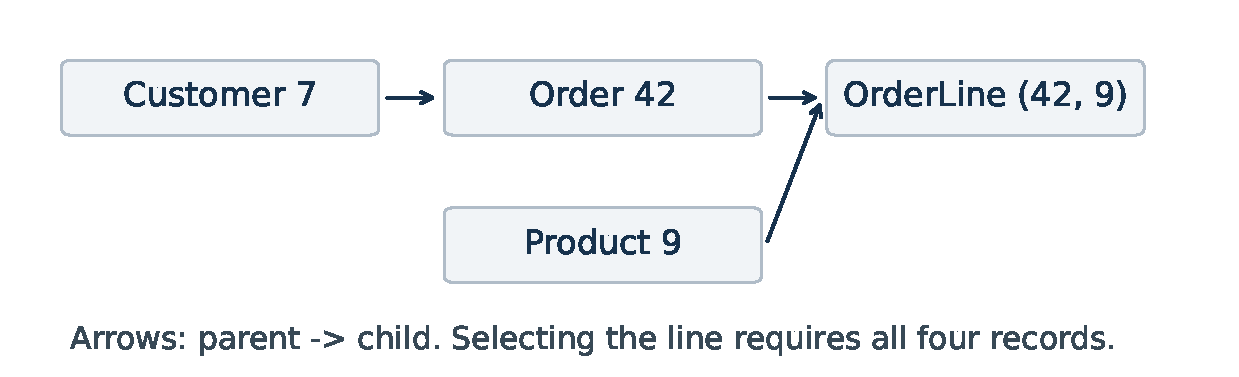
\includegraphics[width=\linewidth]{assets/closure.pdf}\caption{Explanatory four-record closure, not a measured dataset. Selecting the OrderLine requires its Order, Customer and Product.}\end{figure}
With an empty selection this line costs four records. A budget of three rejects it. A budget of four can accept it. Another line with the same already-kept parents can cost only one extra record; two selected child rows do not necessarily cost two complete parent chains.

\section{Candidate sampling and scalability}
\plain{Instead of loading every record identifier into Python, the app considers a bounded pool and tries to avoid expensive scans where keys allow it.}
\technical{Candidate pool size targets $C=\min(N,\max(B,\lceil1.25B\rceil))$. Each nonempty table gets approximately its row-count proportion, rounded upward with at least one key; those per-table minimums can increase the combined pool beyond the nominal target. Tables reuse exact verified counts when available.}

Dense single integer keys may use uniform rejection guesses followed by indexed membership checks. The fast path requires \path{sample_size}$\times4<$ table rows and a key range at most four times the row count; it bounds attempts and falls back to streaming. Sparse, noninteger and composite keys use an exact seeded reservoir over keys ordered by the full PK. FK values are prefetched in batches rather than one lookup per selected row.

The algorithm still performs full-source content fingerprinting for pipeline evidence and may stream full PK indexes for reservoir sampling. ``Bounded candidate memory'' therefore does not mean ``no full database reads'' or ``constant total runtime''.

\section{Method 1: random-repair}
\plain{Shuffle candidate records, then include each one's required parent records if the whole addition fits.}
\technical{The baseline samples candidates, shuffles with random.Random(seed), computes incremental closure and merges accepted rows. Repair is budget-aware at selection time. It does not blindly select a budget of children and then exceed the budget by adding parents.}

\section{Method 2: referential}
\plain{Walk the table relationships from parents toward children, randomly choosing records within that order.}
\technical{This baseline uses a topological parent-first table order and seeded within-table choices with the same dependency closure and feasibility rules. It does not read workload weights. Spending the budget early on parent tables can leave few useful child rows for a specific workload.}

\section{Method 3: workload-aware}
\plain{First try real records that make your queries useful. Then use the remaining space on tables that the declared workload references more heavily.}
\technical{Usable queries produce bounded PK witnesses from their actual FROM, JOIN and WHERE clauses. Query IDs explicitly required by acceptance are visited first in each round. Witnesses are traversed round-robin so one query does not consume all witness space first. Missing-parent closure is prefetched in groups of 64 witnesses and charged incrementally.}

Each query's witness limit is
\[
L=\min\left(1000,\max\left(1,\left\lfloor B/\max(1,Q)\right\rfloor\right)\right),
\]
where $Q$ is the number of usable queries. Remaining sampled candidates receive a static table priority, are shuffled for seeded tie-breaking and visited by descending priority buckets. Candidates are accepted only if their incremental required closure fits.

\section{Actual numeric scoring constants}
For each supported, usable query, the implementation adds:
\begin{longtable}{>{\RaggedRight\arraybackslash}p{.63\linewidth}>{\RaggedRight\arraybackslash}p{.29\linewidth}}
\toprule\textbf{Detected feature} & \textbf{Contribution}\\\midrule\endhead
Every referenced table & $+2.0$ to that table\\[4pt]
Detected join pairs & $+0.5$ per pair to the first referenced table\\[4pt]
Each detected filter column & $+1.0$ to its resolved table\\[4pt]
Each detected grouping column & $+1.5$ to its resolved table\\[4pt]
Any grouping or aggregate in the query & $+1.0$ to the first referenced table\\[4pt]
Table not otherwise weighted & Default weight $1.0$\\\bottomrule
\end{longtable}
These are fixed heuristic coefficients in sampler.py, not learned parameters, measured feature importances or user-tuned model weights. A one-table query with one detected filter and no aggregation contributes $2+1=3$. With a grouping column and aggregation, further resolved group and first-table contributions apply.

\reviewpoint{There is no current ``query gain divided by full closure cost'' optimizer here. The implementation uses bounded real witnesses, static table priorities and exact incremental feasibility. Do not describe it as solving an optimal minimum subset, HAVING satisfiability or general query equivalence.}

\section{Complexity and practical limits}
Let $T$ be table count and $C$ the sampled candidate count. The static priority bucket ordering costs $O(C+T\log T)$ after weights and sampling, rather than sorting every candidate by a recomputed closure ratio. Dependency traversal, database I/O, exact result comparison and full-source fingerprinting add their own costs. Memory holds sampled candidates, selected keys, caches and bounded batches; a large dependency closure can still be expensive. No method is guaranteed to fill every row slot or outperform the others.
\source{src/safeslicesql/sampler.py; src/safeslicesql/dependency_graph.py; src/safeslicesql/workload_candidates.py}

\chapter{Parameters and function contracts}
\section{User controls and defaults}
\begin{longtable}{>{\RaggedRight\arraybackslash}p{.26\linewidth}>{\RaggedRight\arraybackslash}p{.24\linewidth}>{\RaggedRight\arraybackslash}p{.42\linewidth}}
\toprule\textbf{Parameter} & \textbf{Default / range} & \textbf{Effect}\\\midrule\endhead
Input kind & mysql/csv/folder/xlsx & Select an existing schema or text-preserving file-import path.\\[4pt]
Desktop budget & 10; 1--100\% & Hard total-row maximum including required parent rows.\\[4pt]
Method & Desktop: workload-aware & One of random-repair, referential, workload-aware; CLI run requires a method.\\[4pt]
Seed & 42 & Deterministic choices on unchanged data with the same code/backend semantics.\\[4pt]
Custom workload & None in desktop request & Overrides generated structural workload. CLI default is workloads/workload.sql, with source-specific fallback where present; auto generates SQL.\\[4pt]
Compare & False & Run all three methods; the same target is refreshed per run and retains the last successful committed copy.\\[4pt]
Minimum query survival & Desktop 1.0; CLI/library 0.0 & Fraction 0--1 internally. Positive threshold also requires an eligible query denominator.\\[4pt]
Minimum exact retention & 0.0 & Average exact result-row retention threshold, not physical row percentage.\\[4pt]
Required query IDs & Empty tuple/list & Every named query must exist, be supported, execute and survive. Statement order defines Q1, Q2, etc.\\[4pt]
Dry run & False & CLI selects only, without constructing or touching the target.\\\bottomrule
\end{longtable}

\section{Runtime limits from the public template}
Environment keys have the prefix \path{SAFESLICE_LIMIT_}. All values must be positive integers. Byte limits use actual bytes, not decimal MB.
\begin{longtable}{>{\RaggedRight\arraybackslash}p{.46\linewidth}>{\RaggedRight\arraybackslash}p{.19\linewidth}>{\RaggedRight\arraybackslash}p{.27\linewidth}}
\toprule\textbf{Suffix} & \textbf{Default} & \textbf{Meaning}\\\midrule\endhead
JOB\_SECONDS & 600 & Whole cooperative job deadline\\[4pt]
STATEMENT\_SECONDS & 30 & Eligible SELECT/lock/progress timeout\\[4pt]
CONNECT\_SECONDS & 10 & MySQL connect timeout\\[4pt]
MAX\_SOURCE\_ROWS & 5,000,000 & Total source-row guard\\[4pt]
MAX\_RESULT\_ROWS & 1,000,000 & Rows streamed per query\\[4pt]
MAX\_INPUT\_BYTES & 104,857,600 & 100 MiB input / expanded XLSX guard\\[4pt]
MAX\_CELL\_BYTES & 1,048,576 & 1 MiB per imported cell\\[4pt]
MAX\_TEMP\_BYTES & 536,870,912 & 512 MiB temporary comparison database\\[4pt]
MAX\_MEMORY\_BYTES & 1,073,741,824 & 1 GiB client process RSS guard\\[4pt]
MAX\_TABLES & 100 & Reflected/imported table limit\\[4pt]
MAX\_COLUMNS & 500 & Per-table columns, including generated CSV ID\\\bottomrule
\end{longtable}

Memory is sampled at checkpoints, not continuously; a native allocation may exceed a limit before the next check. MySQL eligible SELECT execution time, lock waits and socket timeouts are distinct controls. The socket read/write timeout is statement seconds plus five. These are cooperative bounds, not an OS-level quota or a supported-capacity certificate. Restart the desktop after editing its environment settings.

\section{Important internal batch and guard values}
The candidate multiplier is 1.25; decision log limit is 1,000 entries; witness prefetch is 64; per-query witness cap is 1,000; FK prefetch default is 5,000 keys; materialization and file import use 500-row batches; automatic large-table example queries cap ordered results at 1,000 or the smaller runtime cap. The target lock waits up to five seconds. Record searches allow 25 rows from each side and a maximum query text length of 500 characters. Scale RSS sampling uses a 0.05-second interval.

\section{Core function contracts}
The full exact API appendix follows later; the most useful contracts to understand first are:
\begin{description}[style=nextline,leftmargin=1.5em,labelindent=0pt]
\item[\texttt{prepare\_dataset()}] Takes exactly one input mode, creates owned schemas when needed and returns PreparedDataset with source/target configs, workload path, table counts and manifest. Success retains schemas for later inspection; failure attempts scoped cleanup.
\item[\texttt{inspect\_schema()}] Returns SchemaMetadata. Optional same-view counts avoid redundant counting. Reflection/count failure is an error, not an empty table.
\item[\texttt{build\_dependency\_graph()}] Returns DependencyGraph with parent-to-child edges and self-reference tracking.
\item[\texttt{analyze\_workload()}] Returns WorkloadAnalysis containing QueryInfo entries and support/error status. Main pipeline setup supplies False and evaluates later.
\item[\texttt{select\_rows()}] Returns SelectionResult with the selected keys, their total count, added-parent count, rejected-candidate count and bounded decision log. Workload-aware requires a usable workload. The library default method differs from the desktop request default.
\item[\texttt{compute\_closure()}] Returns ClosureResult with selected rows and added dependencies. satisfied excludes rows already paid for; stop\_after limits work when the remaining budget cannot fit.
\item[\texttt{materialize\_subset()}] Returns GenerationResult. It can return a failed result after rollback; pipeline checks success before claiming a committed copy. The callback is the in-transaction quality checkpoint.
\item[\texttt{evaluate\_workload()}] Returns WorkloadReport with per-query QueryResult records and workload averages. It distinguishes unsupported syntax, execution failures and known source-empty results.
\item[\texttt{validate\_subset()}] Returns ValidationReport. A full snapshot supports unchanged-content evidence. An unchanged count alone leaves source\_unchanged unverified.
\item[\texttt{run\_pipeline()}] Returns BenchmarkRunResult joining selection, generation, validation, workload, acceptance, timings and success/error state. It does not omit evidence merely because an experiment failed.
\item[\texttt{run\_benchmark()}] Returns BenchmarkResults for the matrix, with total/successful/failed run counts and CSV/summary/plot artifacts.
\end{description}

\section{How results travel through the program}
\begin{lstlisting}[language=Python]
CopyRequest
  -> PreparedDataset + run.yaml
  -> SchemaMetadata + DependencyGraph + WorkloadAnalysis
  -> SelectionResult
  -> GenerationResult (pending until checks pass)
  -> WorkloadReport + ValidationReport + AcceptanceReport
  -> BenchmarkRunResult
  -> BenchmarkResults / CopyOutcome
  -> CSV + JSON + charts + readable report
\end{lstlisting}
The data contracts live in types.py and the acceptance, desktop-service and input-preparation modules. In particular, success, is\_valid, acceptance.passed and a saved summary's ready flag answer related but different questions. Always read the recorded error fields before explaining a failed or historical result.

\chapter{Metrics: formulas, meanings and edge cases}
\section{Integrity metrics}
\plain{First ask whether the smaller copy is a legal and faithful selection of records. This is independent from how many query answers it keeps.}
\begin{itemize}
\item \textbf{PK uniqueness:} no duplicate tuple across all declared primary-key columns.
\item \textbf{FK violations:} non-null retained child references without a matching retained parent. Zero is required; the total can count violations of separate relationships, not necessarily unique bad child rows.
\item \textbf{Budget compliance:} actual rows across every target table do not exceed $B$.
\item \textbf{Schema compatibility:} expected tables, columns, PK/FK definitions, unique/check constraints and indexes match reflected source definitions.
\item \textbf{Copied-value equality:} materialization compares every inserted batch back to the source; read-only evidence actions can check current copied records again.
\item \textbf{Source unchanged:} True/False/None. None means history is unverified; it must not be described as verified unchanged.
\end{itemize}
ValidationReport.is\_valid requires unique PKs, zero FK violations, a compliant budget, compatible schema, no missing tables or check errors, and source\_unchanged not False. It permits None as structural validity with unverified history. The normal pipeline provides a baseline; standalone CLI validation does not recreate past history.

\section{Query survival}
For supported queries, a query survives when source and target both return at least one row. Let $E$ be eligible supported queries: known nonempty source results plus failures where the source result is unknown. Known source-empty queries are excluded from this denominator.
\[
\operatorname{survival}=\frac{\#\{q\in E: q\text{ survives}\}}{|E|}.
\]
When $|E|=0$, the stored rate is 0.0. An execution error remains a failed measurement; unsupported syntax is instead excluded with a reason. A positive minimum survival gate rejects a workload that cannot demonstrate eligible survival.

\textbf{Subtle example:} SELECT COUNT(*) returns one row even if the underlying table has zero records. It can therefore survive while its numeric answer changes. Query survival measures nonempty returned results, not semantic equivalence or a promise that all selected tables contain data.

\section{Exact result-row retention}
Let $m_S(v)$ and $m_T(v)$ be the multiplicities of typed output tuple $v$ in source and target results. For a nonempty source result,
\[
R_{\mathrm{row}}=\frac{\sum_v\min\{m_S(v),m_T(v)\}}{\sum_v m_S(v)}.
\]
This is multiset intersection, so duplicates count correctly. Output columns are compared by ordinal position, preserving duplicate column labels. Type names and string representations encode driver-returned values; ordering is ignored. This is not approximate similarity, sampled comparison or equality of just the first few rows.

\section{Key retention and grouping retention}
\textbf{Key retention} is the fraction of distinct declared projected source key tuples still present in the target result. It uses PK lineage and aliases, not a column-name suffix such as ``id''. If a safe key mapping is unavailable, the implementation falls back to exact row retention.

\textbf{Aggregate retention} normally measures the survival of distinct projected grouping-key tuples, when every grouping expression can be mapped safely to an output position. It measures \emph{group coverage}, not closeness of SUM, AVG or COUNT values. A scalar aggregate or unprojected/ambiguous group falls back to exact row retention.

For example, North and South might both remain after slicing, so group coverage can be 100 percent, while both revenue totals decrease. An unchanged invoice's stored total need not equal the sum of its retained line items because not all children are required by retaining a parent.

\section{Workload averages, failures and empty outputs}
Overall key, row and aggregate retention are arithmetic means across all supported queries, not weighted by result-set row count. Unsupported queries are not in those means. Failed supported evaluations contribute zero. If source and target are both empty, each retention score is 1.0, survival is False and that query is excluded only from the survival denominator. If a source query fails and no successful baseline proves it empty, it remains an unknown-source failure in the survival denominator.

Reports expose total, supported, excluded, failed, known source-nonempty, source-unknown and survival-denominator counts. Those counts are essential for assessing a percentage. A high score from one trivial aggregate should not hide excluded critical SQL.

\section{Selection diagnostics and size reduction}
Selection reports \path{total_selected}, \path{closure_additions} and \path{rejected_candidates}. Closure additions are additional parent records attributed during selection, not a separate new row budget. A rejection means an attempted closure could not fit; it is not itself an FK violation. The physical retained fraction is \path{actual_rows}/$N$, and row reduction is $1-\text{actual\_rows}/N$ when $N>0$. Neither should be confused with average query result retention.

\section{Timing and benchmark statistics}
The run-level total is the sum of recorded preflight, selection, materialization, workload-evaluation and validation timings. Materialization timing subtracts the nested before-commit evaluation/validation timings to avoid double-counting. CLI runs add their initial source setup cost to preflight. Benchmark matrices share an initial source setup outside individual trial timing, so a per-trial runtime is not the wall time of launching the entire experiment suite.

Per-query source/target execution times include connection/query fetching/streaming; temporary-store ingestion/comparison times are recorded separately and subtracted from those fetch timings. Export, charts, UI rendering and connection setup outside the timed stages are not automatically included in an individual stage total.

Benchmark summaries group by method and budget. They report attempted/successful/failed counts, then calculate mean, sample standard deviation and observation count using only successful measured runs. Missing metrics stay missing. One successful run has no sample standard deviation; an all-failed group has no valid performance mean. Fewer failed runs can matter more than a faster mean from the survivors.

\section{What metrics are absent}
No classification accuracy, precision/recall/F1, learned loss, numerical aggregate-error percentage, universal query-equivalence proof or total MySQL server resource profile is implemented as a standard project metric. Do not add these names to a review slide as if the software measured them. If needed, design and label an additional experiment separately.
\source{src/safeslicesql/validator.py; src/safeslicesql/result_store.py; src/safeslicesql/types.py; src/safeslicesql/benchmark.py}

\chapter{Measured evidence: fresh checks and saved results}

\section{How to read evidence honestly}

Fresh checks below were run while preparing this guide on 25 November 2026. Saved database results were read from local artifacts; those database jobs were not rerun. Artifact modification dates are not embedded experiment timestamps. Historical files without a source-commit identifier cannot establish performance of this exact code revision. No live private MySQL credentials were printed or reproduced.

\section{Fresh verification of the current checkout}

\begin{longtable}{>{\raggedright\arraybackslash}p{0.258\linewidth}>{\raggedright\arraybackslash}p{0.294\linewidth}>{\raggedright\arraybackslash}p{0.368\linewidth}}
\toprule
\textbf{Check} & \textbf{Observed result} & \textbf{Interpretation} \\
\midrule
\endfirsthead
\toprule
\textbf{Check} & \textbf{Observed result} & \textbf{Interpretation} \\
\midrule
\endhead
Python 3.12 pytest, marker not db & 368 passed; 0 failures/errors; 32 deselected. Wall time reported by pytest: 104.49 s. & Current non-database tests passed. Deselected db tests are not fresh MySQL evidence. \\[4pt]
Ruff check . & All checks passed. & Static checks passed for the inspected checkout before adding these document artifacts. \\[4pt]
SQLite generated-schema self-test & 30 checks; 0 failures; seed 42; 5 shapes; up to 100 rows/table. & Checks all methods at 10 and 100 percent, replay equality and full-budget result equality. \\[4pt]
\bottomrule
\end{longtable}


\section{A saved 20-row demo: why survival and retention differ}

Source artifact: \path{results/readme-demo-1d9302050e/copy_summary.json}. Recorded UTC timestamp: 2026-11-22T06:15:03.855032+00:00. The copy retained 5 of 20 rows at a 25-percent budget, with unique PKs, zero FK violations, matching schema and a verified source read view.

\begin{longtable}{>{\raggedright\arraybackslash}p{0.129\linewidth}>{\raggedright\arraybackslash}p{0.331\linewidth}>{\raggedright\arraybackslash}p{0.184\linewidth}>{\raggedright\arraybackslash}p{0.276\linewidth}}
\toprule
\textbf{Query} & \textbf{Source / target result rows} & \textbf{Survived} & \textbf{Exact row retention} \\
\midrule
\endfirsthead
\toprule
\textbf{Query} & \textbf{Source / target result rows} & \textbf{Survived} & \textbf{Exact row retention} \\
\midrule
\endhead
Q1 & 20 / 5 & True & 25.00\% \\[4pt]
Q2 & 1 / 1 & True & 0.00\% \\[4pt]
Q3 & 20 / 5 & True & 25.00\% \\[4pt]
\bottomrule
\end{longtable}


\[\text{Average exact retention}=(0.25+0+0.25)/3=0.1667.\]

All three queries return a row set, so query survival is 100 percent. The scalar COUNT query returns one row on both sides, yet its value changes from 20 to 5, so exact result retention for that query is zero. The overall 16.67 percent is an average over queries; it is not the 25-percent physical row fraction.

\section{Historical World comparison: 18 saved runs}

Source: \path{results/raw/all_benchmark_runs.csv}. File modified UTC date: 2026-11-02. There are 18 saved successful runs: three methods, budgets 10/20/30 percent and seeds 42/123 on 5,302 source rows. This artifact predates the current source snapshot and has no runtime\_preflight column. Treat its runtime as the recorded older stage total, not a current end-to-end latency guarantee.

\begin{figure}[htbp]\centering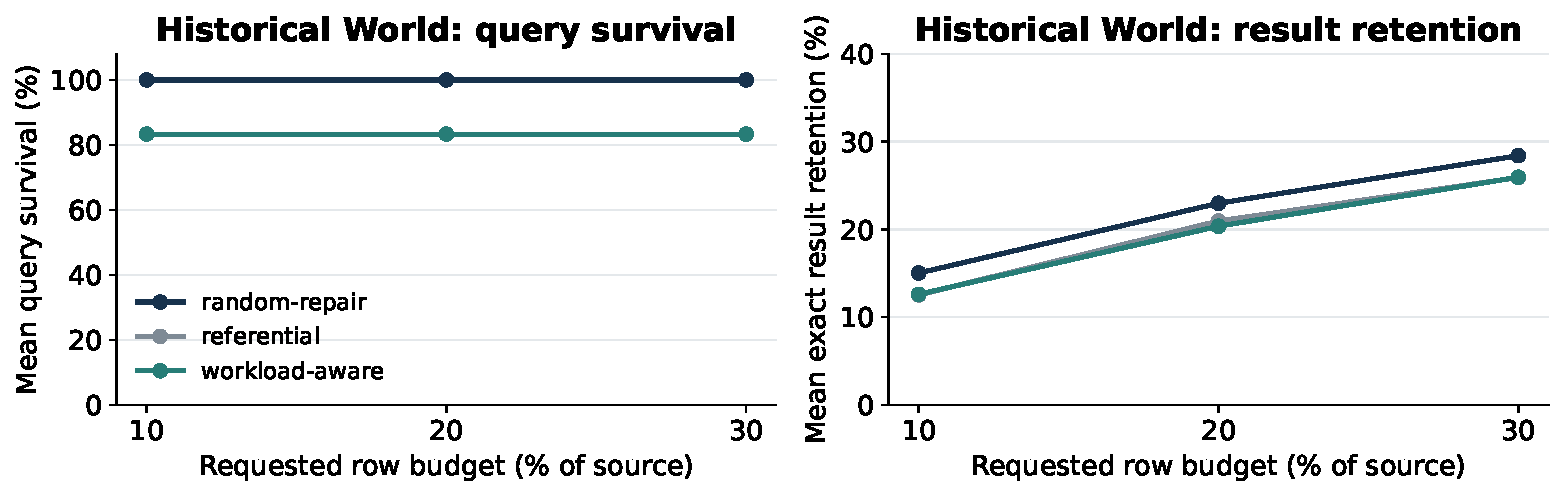
\includegraphics[width=\linewidth]{assets/historical-world.pdf}\caption{Historical World means, two seeds per method and budget. Source: local all\_benchmark\_runs.csv; artifact date 2026-11-02. These plots describe saved runs, not a new performance comparison.}\end{figure}

\begin{longtable}{>{\raggedright\arraybackslash}p{0.258\linewidth}>{\raggedright\arraybackslash}p{0.055\linewidth}>{\raggedright\arraybackslash}p{0.147\linewidth}>{\raggedright\arraybackslash}p{0.156\linewidth}>{\raggedright\arraybackslash}p{0.156\linewidth}>{\raggedright\arraybackslash}p{0.147\linewidth}}
\toprule
\textbf{Method / budget} & \textbf{n} & \textbf{Survival} & \textbf{Exact retention} & \textbf{Group metric} & \textbf{Saved time} \\
\midrule
\endfirsthead
\toprule
\textbf{Method / budget} & \textbf{n} & \textbf{Survival} & \textbf{Exact retention} & \textbf{Group metric} & \textbf{Saved time} \\
\midrule
\endhead
random-repair / 10\% & 2 & 100.00\% & 15.03\% & 47.17\% & 0.461 s \\[4pt]
random-repair / 20\% & 2 & 100.00\% & 22.98\% & 55.13\% & 0.486 s \\[4pt]
random-repair / 30\% & 2 & 100.00\% & 28.40\% & 61.74\% & 0.540 s \\[4pt]
referential / 10\% & 2 & 83.33\% & 12.53\% & 45.87\% & 0.417 s \\[4pt]
referential / 20\% & 2 & 83.33\% & 20.95\% & 53.10\% & 0.466 s \\[4pt]
referential / 30\% & 2 & 83.33\% & 25.92\% & 59.25\% & 0.546 s \\[4pt]
workload-aware / 10\% & 2 & 83.33\% & 12.60\% & 45.94\% & 0.405 s \\[4pt]
workload-aware / 20\% & 2 & 83.33\% & 20.36\% & 52.51\% & 0.495 s \\[4pt]
workload-aware / 30\% & 2 & 83.33\% & 25.95\% & 59.29\% & 0.559 s \\[4pt]
\bottomrule
\end{longtable}


In this saved artifact random-repair has higher mean survival and exact retention than workload-aware selection. This is useful evidence that the proposed heuristic is not guaranteed to win. Two seeds do not establish statistical superiority; rerun the current code with the same source/workload, broader seeds and explicit acceptance before making comparative claims.

\section{Saved MySQL synthetic scale evidence}

Source: \path{results/scale/6893236af2c9/evidence.json}. State: completed; backend: MySQL; Python: 3.10.11. This recorded run covers 5 shapes and 30 checks per scale sample. The requested row scale is a per-table generation bound, not a total-database row count.

\begin{longtable}{>{\raggedright\arraybackslash}p{0.138\linewidth}>{\raggedright\arraybackslash}p{0.322\linewidth}>{\raggedright\arraybackslash}p{0.138\linewidth}>{\raggedright\arraybackslash}p{0.175\linewidth}>{\raggedright\arraybackslash}p{0.147\linewidth}}
\toprule
\textbf{Rows/table bound} & \textbf{Actual source totals by case} & \textbf{Checks / failures} & \textbf{Wall / CPU time} & \textbf{Peak client RSS} \\
\midrule
\endfirsthead
\toprule
\textbf{Rows/table bound} & \textbf{Actual source totals by case} & \textbf{Checks / failures} & \textbf{Wall / CPU time} & \textbf{Peak client RSS} \\
\midrule
\endhead
1000 & 1,446, 1,930, 3,558, 2,794, 1,051 & 30 / 0 & 73.93 / 50.42 s & 174.69 MiB \\[4pt]
10000 & 15,649, 17,077, 40,463, 31,236, 12,321 & 30 / 0 & 426.58 / 342.59 s & 262.73 MiB \\[4pt]
\bottomrule
\end{longtable}


The largest recorded case here has 40,463 total source rows and a sampled client-process peak of about 262.73 MiB for its scale sample. The measure excludes MySQL server resource use and is a sampled process peak, not a continuous exact maximum. It is explicitly synthetic evidence with production\_certification=False.

\section{What has not been established}

The project does not contain a current production-capacity certification, a guarantee that every database in the download list has been sliced end to end, a universal method winner, or a classification F1/FN evaluation. A 5,000,000-row resource policy is a configurable guard, not evidence of a successful five-million-row benchmark. The sanitized evidence snapshot and source hashes accompany this guide so each reported value remains traceable.

\chapter{Safety, recovery and operational boundaries}
\section{What protects the original and the last valid copy}
\plain{The original is read, the output is separate, and a failed replacement should not wipe out an earlier valid output.}
\technical{Actual connected identity checks prevent source=target even through MySQL hostname aliases. Read-only sessions are installed on app-created source engines. Schema reproduction rejects unrelated target tables, pre-existing target triggers and incompatible definitions before writes. DML refresh uses one transaction, and acceptance failure rolls it back. A MySQL named lock or SQLite file lock coordinates participating SafeSliceSQL writers.}

These controls do not prevent arbitrary external target writers or concurrent DDL; use a dedicated target and avoid schema changes during a run. Creating an arbitrary SQLAlchemy engine outside \path{bounded_engine()} does not install its event hooks automatically.

\section{Journal state and interruption}
Jobs record running phases and terminal outcomes such as completed, failed, rejected or interrupted. A cancellation uses a dedicated interruption exception that unwinds transactions. If a process dies, recovery verifies owner/host/process identity before marking its running job interrupted. It does not approve, resume or complete partially executed SQL.

Cancellation before commit restores previous target rows; cancellation arriving after commit cannot undo a successful commit. A pending schema creation intent without a confirmed ownership record is not automatically deleted. That distinction prevents cleanup from guessing at ownership after a hard crash.

\section{Credentials and deployment}
Source and target accounts should have separate least-privilege roles. The public grant script is an administrator-reviewed example and is never automatically executed. Prefix-grant behavior depends on MySQL partial-revoke configuration and correct escaping; exact schema grants may be needed.

Passwords may come from private environment values, a private secret file or an approved native OS vault. Explicit references that cannot be read fail rather than silently falling back. Logs redact registered secrets and suppress SQL/bound-value text in public database errors. Reports can still contain input paths, schema names and workload literals, and copied rows contain original data.

\reviewpoint{The project is not a PII masker, encryption system, remote authentication service or multi-user authorization platform. Its current strengths are checked subsetting, transaction-aware quality gates, reproducibility and inspectable evidence.}

\section{Ownership-aware cleanup}
\begin{lstlisting}[language={}]
safeslice jobs list
safeslice jobs recover
safeslice jobs cleanup --days 7
\end{lstlisting}
Cleanup verifies the terminal job belongs to the current local user/host, the schema name exactly matches an owned generated pattern, the recorded server UUID matches, and the retention age is satisfied. It keeps report files. It does not drop arbitrary named CLI targets or a user-selected original source. These local ownership checks are accident prevention, not tamper-proof authentication against a person who can edit the job files.

\chapter{Runbook: demonstrate and verify the whole project}
\section{Start the desktop}
Open PowerShell in the checkout. The virtual environment and environment file already exist locally; another machine must complete README installation first. A running MySQL server is required for desktop inputs, including CSVs.
\begin{lstlisting}[language={}]
cd C:\Users\saivi\Projects\SafeSliceSQL
.\demo.bat
\end{lstlisting}
If the window fails to open, launch with the console interpreter to see diagnostics:
\begin{lstlisting}[language={}]
.\.venv\Scripts\python.exe -m safeslicesql.desktop
\end{lstlisting}
Select Diamonds CSV for a source above 5,000 rows, set 10 percent, choose \path{testing_diamonds}.sql in Options and create the copy. Expect at most 5,394 copied rows. Inspect Results, Verify my copy, charts and an exported report. To demonstrate FK preservation, use World or Chinook after importing the matching MySQL dump and choose its matching SQL workload.

\section{CLI: inspect, preview, copy and validate}
Use a dedicated disposable target created in MySQL for CLI runs. Replace connection details in the private environment file; do not paste passwords into shell examples. The commands below use an activated environment or the installed safeslice entry point.
\begin{lstlisting}[language=SQL]
CREATE DATABASE IF NOT EXISTS world_review_slice;
\end{lstlisting}
\begin{lstlisting}[language={}]
safeslice inspect --database world

safeslice run --method workload-aware --budget-percent 20 --seed 42 --source world --target world_review_slice --workload workloads/testing_world.sql --dry-run

safeslice run --method workload-aware --budget-percent 20 --seed 42 --source world --target world_review_slice --workload workloads/testing_world.sql --min-query-survival 1.0 --required-query Q2 --output-dir results/manual-review

safeslice validate --source world --target world_review_slice --budget-limit 1060 --workload workloads/testing_world.sql
\end{lstlisting}
The --budget-limit on standalone validation must be the experiment's row budget. Without it the CLI defaults to the full current source size; that would not demonstrate compliance with the requested 20-percent slice. A standalone validate result also cannot reconstruct source history at creation time. If an explicit acceptance threshold rejects, inspect the recorded reason and adjust the workload/budget for a new run.

\section{A reproducible comparison}
Choose the same input, declared workload, percentage and seeds for every method. The checked-in World YAML requests 18 experiments; the SQLite example requests 27. Review source/target configuration and output paths first.
\begin{lstlisting}[language={}]
safeslice benchmark --config benchmarks/benchmarks_world.yaml
\end{lstlisting}
The target is refreshed for each run. Per-query CSVs explain exclusions, errors and lost results; raw combined CSVs retain failed attempts. Summaries and charts include successful measurement counts and missing standard deviations honestly. Do not describe the target left after comparison as a merged copy from every strategy.

\section{Validation and scale checks}
\begin{lstlisting}[language={}]
python -m pytest -m "not db" -q --tb=short
python -m ruff check .
safeslice selftest --cases 5 --rows 100 --seed 42
safeslice scalecheck --rows 1000 --rows 5000 --seed 42 --cases 5
\end{lstlisting}
Use --mysql only on a disposable test server with permission to create/delete uniquely named test schemas. The scalecheck row setting is a bound per generated table; evidence.json records actual total rows by case. CI configures these checks, but a configured workflow is not proof that a hosted run passed.

\section{Five-minute demonstration sequence}
\begin{enumerate}
\item Explain the source, workload and hard total-row budget. Show exact input preview counts.
\item Show one child-parent relationship and why retaining the child requires the parent.
\item Run the slice with a fixed seed and an explicit quality threshold.
\item Show actual row count versus allowed budget and zero FK violations.
\item Inspect a copied record beside its original, then follow its parent connection.
\item Show per-query survival and exact retention, including a changed aggregate.
\item Export the report and identify its recorded timestamp. If showing a saved report, say that it is saved evidence.
\end{enumerate}

\chapter{What to highlight in a project review}
\section{The strongest defensible story}
\begin{enumerate}
\item \textbf{Problem and invariant:} a useful smaller relational database must preserve required parents while staying within a hard budget.
\item \textbf{Shared baseline framework:} random-repair, referential and workload-aware selectors use the same closure, budget enforcement, materializer, validator and metrics. This makes comparisons more interpretable.
\item \textbf{Workload-aware contribution:} real filter/join witnesses are considered first; table features prioritize remaining candidates; closure cost is checked incrementally.
\item \textbf{Correctness before commit:} copied-value checks, structural checks and workload acceptance happen before the target DML transaction commits.
\item \textbf{Clear metrics:} survival, exact row retention, key retention and grouping coverage measure different things and expose errors/exclusions.
\item \textbf{Engineering completeness:} desktop/CLI share the core, imports support unfamiliar input, jobs are journaled, stops unwind safely and saved evidence is inspectable.
\item \textbf{Evidence with boundaries:} fresh tests, recorded MySQL scale checks and historical method comparisons are distinguished; the heuristic is not claimed to always win.
\end{enumerate}

\section{Likely questions and clear answers}
\begin{description}[style=nextline,leftmargin=1.5em,labelindent=0pt]
\item[Why not choose a random 10 percent of every table?] Independent sampling can create orphan records. Required parent closure must be included and charged to the same total budget.
\item[Does preserving relationships preserve every SQL answer?] No. It prevents missing required parents, but child rows, groups and aggregate inputs may be omitted. The workload is measured separately and can be gated.
\item[Is workload-aware selection a learned model?] No. It is a seeded heuristic with actual query witnesses and fixed coefficients. No training dataset or learned parameters exist.
\item[Why use three methods?] Two baselines help test whether the proposed priority actually improves the declared workload under matched conditions. A fair experiment is allowed to show a baseline winning.
\item[What if a child needs too many parents?] Its incremental closure is rejected if it cannot fit. The algorithm may leave unused space rather than exceed the budget or break a dependency.
\item[Can a composite primary key be used?] Yes. Every key column participates in identity, lookup and ordering. Composite foreign keys remain unsupported.
\item[Why is CSV different from MySQL input?] CSV has no declared relational schema. The import preserves text and adds IDs; use an existing MySQL schema to test real types and FKs.
\item[Is 100-percent survival enough?] No. COUNT can return a row while its value changes, and excluded queries need inspection. Review exact retention, grouping coverage, query errors and required IDs too.
\item[Can rollback undo schema creation?] MySQL DML rollback protects previous row contents. DDL is not transactional; handled cleanup is scoped, and hard crashes may leave schema remnants.
\item[How big a database can it handle?] A configurable source limit is not capacity evidence. Cite actual recorded rows, backend, timing and client RSS, then test representative schemas before promising a size.
\end{description}

\section{Limitations and sensible next experiments}
Present the supported schema/SQL subset explicitly. Expand current-version benchmark seeds and real application workloads; include failure rates and end-to-end setup cost. Test the selected large downloads end to end before certifying them. If numerical aggregate accuracy matters, define and implement a separate metric. More sophisticated marginal-gain selection, cyclic/composite-FK support, masking and multi-user service controls would be future work, not hidden current features.

\reviewpoint{A strong review explains the actual implementation, demonstrates both a kept relationship and a changed query answer, cites measured evidence, and states limitations without inventing guarantees.}

\addtocontents{toc}{\protect\setcounter{tocdepth}{0}}
\appendix
\chapter{Application files: plain language and technical atlas}

\begingroup\setlength{\parskip}{4pt}

Every application module is described below. Paths are relative to the repository root. The function appendix gives exact signatures from the inspected source; private helpers are included there too.

\Needspace{10\baselineskip}

\section{\_\_init\_\_.py}

\textbf{Role:} Package identity\quad\textbf{Size:} 35 source lines.

\plain{Identifies the installed application and exposes its main library operations.}

\technical{Defines version 0.1.0 and re-exports the public configuration, schema, graph, selection, materialization, validation, workload and source-snapshot interfaces through \_\_all\_\_. It is not the launcher or pipeline implementation.}

\textbf{Reads/calls project modules:} \path{config.py}, \path{dependency_graph.py}, \path{sampler.py}, \path{schema_analyzer.py}, \path{source_snapshot.py}, \path{subset_generator.py}, \path{validator.py}, \path{workload_analyzer.py}.

\Needspace{10\baselineskip}

\section{desktop.py}

\textbf{Role:} Desktop entry and controls\quad\textbf{Size:} 1011 source lines.

\plain{Provides the window where you choose data, set the copy size, start work, cancel, and inspect results.}

\technical{The Tkinter Desktop class manages a worker thread, a queue polled by the UI, input preview, quality settings, history and verification actions. main() loads configuration and starts the Tk event loop; expensive operations are delegated to services.}

\textbf{Reads/calls project modules:} \path{config.py}, \path{copy_evidence.py}, \path{desktop_service.py}, \path{input_picker.py}, \path{input_preview.py}, \path{jobs.py}, \path{logging_config.py}, \path{record_browser.py}, \path{result_views.py}, \path{runtime.py}, \path{sampler.py}, \path{saved_results.py}, \path{security.py}, \path{user_errors.py}.

\textbf{Primary entry points/data:} \path{Desktop}, \path{main}.

\Needspace{10\baselineskip}

\section{desktop\_service.py}

\textbf{Role:} Desktop-to-core adapter\quad\textbf{Size:} 129 source lines.

\plain{Turns choices in the window into a real, checked copy job.}

\technical{CopyRequest validates input kind, percentage, method, workload and acceptance. \path{create_copy()} establishes journal and runtime contexts; \_\path{create_copy()} prepares data, writes YAML, opens engines, invokes \path{run_benchmark()}, saves the summary, and disposes engines.}

\textbf{Reads/calls project modules:} \path{acceptance.py}, \path{benchmark.py}, \path{config.py}, \path{dataset_input.py}, \path{experiment_config.py}, \path{jobs.py}, \path{runtime.py}, \path{sampler.py}, \path{saved_results.py}, \path{types.py}.

\textbf{Primary entry points/data:} \path{CopyRequest}, \path{CopyOutcome}, \path{create_copy}.

\Needspace{10\baselineskip}

\section{cli.py}

\textbf{Role:} Command-line entry\quad\textbf{Size:} 741 source lines.

\plain{Lets you inspect, slice, validate, benchmark, self-test and manage jobs from a terminal.}

\technical{Typer app registers commands. run() distinguishes selection-only dry runs from target-changing runs, establishes the source read view, inspects schema, parses SQL and invokes \path{run_pipeline()}. validate() can evaluate a workload but lacks a historical source fingerprint unless supplied through the library.}

\textbf{Reads/calls project modules:} \path{acceptance.py}, \path{automatic_workload.py}, \path{benchmark.py}, \path{commands.py}, \path{config.py}, \path{connection_scope.py}, \path{db.py}, \path{demo.py}, \path{dependency_graph.py}, \path{desktop.py}, \path{jobs.py}, \path{logging_config.py}, \path{pipeline.py}, \path{reporting.py}, \path{runtime.py}, \path{sampler.py}, \path{scale_check.py}, \path{schema_analyzer.py}, \path{security.py}, \path{source_snapshot.py}, \path{synthetic.py}, \path{validator.py}, \path{workload_analyzer.py}.

\textbf{Primary entry points/data:} \path{inspect}, \path{run}, \path{validate}, \path{benchmark}, \path{selftest}, \path{scalecheck}, \path{jobs}, \path{store_password}, \path{desktop}, \path{demo}.

\Needspace{10\baselineskip}

\section{demo.py}

\textbf{Role:} Terminal presentation menu\quad\textbf{Size:} 374 source lines.

\plain{Offers a numbered menu around the same application so a demonstration needs fewer typed commands.}

\technical{DemoSettings carries source, target, workload, budget, method and seed. The menu calls existing CLI entry points using argument lists rather than shell interpolation, prepares unfamiliar input and creates benchmark YAML.}

\textbf{Reads/calls project modules:} \path{config.py}, \path{dataset_input.py}, \path{experiment_config.py}, \path{input_picker.py}, \path{sampler.py}, \path{security.py}.

\textbf{Primary entry points/data:} \path{DemoSettings}, \path{interactive_demo}.

\Needspace{10\baselineskip}

\section{commands.py}

\textbf{Role:} CLI operation wrapper\quad\textbf{Size:} 39 source lines.

\plain{Gives terminal actions a consistent job record, limits and stop behavior.}

\technical{\path{bounded_command} decorates commands with Limits.\path{from_env()}, journal() and \path{execution_context()}. Cancellation/keyboard interrupts exit 130, cooperative limit stops exit 124, and invalid values exit 1.}

\textbf{Reads/calls project modules:} \path{config.py}, \path{jobs.py}, \path{runtime.py}, \path{security.py}.

\textbf{Primary entry points/data:} \path{bounded_command}.

\Needspace{10\baselineskip}

\section{config.py}

\textbf{Role:} Configuration and URLs\quad\textbf{Size:} 212 source lines.

\plain{Reads connection details and rejects incomplete or conflicting settings.}

\technical{DatabaseConfig exposes a SQLAlchemy URL object and masks password representation. AppConfig separates source and target. \path{load_config()} loads the project-relative environment and delegates secret resolution; \path{require_target}=False supports source-only actions.}

\textbf{Reads/calls project modules:} \path{security.py}.

\textbf{Primary entry points/data:} \path{DatabaseConfig}, \path{AppConfig}, \path{load_logging_settings}, \path{load_config}.

\Needspace{10\baselineskip}

\section{db.py}

\textbf{Role:} Connections and identity\quad\textbf{Size:} 211 source lines.

\plain{Connects to the correct servers and prevents the original database from being used as the output.}

\technical{Builds engines, tests connections, safely quotes identifiers and counts rows. \path{assert_distinct_databases()} checks actual connected identity; MySQL uses server UUID plus schema, so hostname aliases do not bypass protection.}

\textbf{Reads/calls project modules:} \path{config.py}, \path{runtime.py}.

\textbf{Primary entry points/data:} \path{assert_distinct_databases}, \path{create_engine}, \path{get_source_engine}, \path{get_target_engine}, \path{test_connection}, \path{quote_ident}, \path{get_row_count}.

\Needspace{10\baselineskip}

\section{connection\_scope.py}

\textbf{Role:} Shared source read view\quad\textbf{Size:} 50 source lines.

\plain{Keeps all stages looking at the same version of the original data.}

\technical{ConnectionScope borrows a SQLAlchemy connection without closing its transaction when helpers exit. \path{source_transaction()} establishes a repeatable-read MySQL transaction or reuses an existing scope. Cached verified snapshots/counts travel with the scope.}

\textbf{Primary entry points/data:} \path{ConnectionScope}, \path{inspect_scope}, \path{source_transaction}.

\Needspace{10\baselineskip}

\section{security.py}

\textbf{Role:} Secrets and safe errors\quad\textbf{Size:} 80 source lines.

\plain{Keeps passwords out of ordinary messages and can read them from a protected file or OS vault.}

\technical{credential() chooses a configured file or approved native keyring backend, otherwise the environment password. Explicit unreadable references fail closed. \path{remember_secret()}, redact() and \path{safe_error()} remove registered secrets and SQL/bound-value details from public errors.}

\textbf{Primary entry points/data:} \path{os_vault}, \path{remember_secret}, \path{redact}, \path{safe_error}, \path{credential}.

\Needspace{10\baselineskip}

\section{logging\_config.py}

\textbf{Role:} Diagnostics\quad\textbf{Size:} 129 source lines.

\plain{Writes useful progress and debug information without displaying passwords.}

\technical{Installs project logger levels, a concise console handler, a rotating diagnostic file and RedactionFilter. Logs are diagnostics, not experimental evidence by themselves.}

\textbf{Reads/calls project modules:} \path{security.py}.

\textbf{Primary entry points/data:} \path{RedactionFilter}, \path{ConsoleHandler}, \path{setup_logging}.

\Needspace{10\baselineskip}

\section{input\_picker.py}

\textbf{Role:} Input selection\quad\textbf{Size:} 43 source lines.

\plain{Shows the file chooser or available user databases.}

\technical{\path{available_databases()} filters system schemas and disposes its connection. \path{pick_input()} handles Tk file/folder dialogs and cancellation without preparing or changing a dataset.}

\textbf{Reads/calls project modules:} \path{config.py}, \path{runtime.py}.

\textbf{Primary entry points/data:} \path{available_databases}, \path{pick_input}.

\Needspace{10\baselineskip}

\section{input\_preview.py}

\textbf{Role:} Preview before writes\quad\textbf{Size:} 70 source lines.

\plain{Shows how many rows and columns an input contains before creating databases.}

\technical{\path{preview_input()} uses the same streaming file reader as import or a read-only source engine. InputPreview.\path{row_budget()} mirrors percentage rounding and reports zero for an empty input.}

\textbf{Reads/calls project modules:} \path{dataset_input.py}, \path{runtime.py}, \path{schema_analyzer.py}.

\textbf{Primary entry points/data:} \path{InputPreview}, \path{preview_input}.

\Needspace{10\baselineskip}

\section{dataset\_input.py}

\textbf{Role:} File import and source preparation\quad\textbf{Size:} 274 source lines.

\plain{Makes a private working database for CSV/Excel input, or connects to an already imported MySQL database.}

\technical{\path{iter_input_tables()} supports CSV, CSV folders and XLSX; \_\path{load_table()} preserves cell strings in text/LONGTEXT columns and assigns \_\path{safeslice_id}. \path{prepare_dataset()} creates UUID-named owned schemas, generates workload SQL, writes dataset.json and attempts scoped cleanup on failure.}

\textbf{Reads/calls project modules:} \path{automatic_workload.py}, \path{config.py}, \path{db.py}, \path{jobs.py}, \path{runtime.py}, \path{schema_analyzer.py}, \path{security.py}.

\textbf{Primary entry points/data:} \path{PreparedDataset}, \path{iter_input_tables}, \path{import_files}, \path{prepare_dataset}.

\Needspace{10\baselineskip}

\section{automatic\_workload.py}

\textbf{Role:} Automatic example SQL\quad\textbf{Size:} 83 source lines.

\plain{Creates basic checks using the table and relationship names actually found in your input.}

\technical{\path{generate_workload()} emits projections, COUNT, category/FK groups, inner joins and non-null FK filters. Large table projections are ordered and bounded by min(1000, \path{max_result_rows}). These queries demonstrate structure rather than infer business priorities.}

\textbf{Reads/calls project modules:} \path{db.py}, \path{dependency_graph.py}, \path{runtime.py}, \path{types.py}.

\textbf{Primary entry points/data:} \path{generate_workload}, \path{save_automatic_workload}.

\Needspace{10\baselineskip}

\section{experiment\_config.py}

\textbf{Role:} One YAML writer\quad\textbf{Size:} 36 source lines.

\plain{Saves the choices needed to repeat a desktop or menu experiment.}

\technical{\path{write_experiment_config()} writes method, budget and seed matrices, a workload path, output directories and optional acceptance thresholds. It does not store database passwords.}

\textbf{Primary entry points/data:} \path{write_experiment_config}.

\Needspace{10\baselineskip}

\section{schema\_analyzer.py}

\textbf{Role:} Schema discovery\quad\textbf{Size:} 194 source lines.

\plain{Finds each table, its record identifier, relationships and exact size.}

\technical{\path{inspect_schema()} reflects columns, PK/FK constraints and exact counts or reuses same-view counts. It marks missing PKs, composite FKs and cross-table cycles unsupported and enforces source/table/column limits.}

\textbf{Reads/calls project modules:} \path{db.py}, \path{dependency_graph.py}, \path{runtime.py}, \path{types.py}.

\textbf{Primary entry points/data:} \path{inspect_schema}.

\Needspace{10\baselineskip}

\section{schema\_compatibility.py}

\textbf{Role:} Schema comparison\quad\textbf{Size:} 104 source lines.

\plain{Checks that the smaller database has the same table rules as the original.}

\technical{\path{table_schema_differences()} compares columns including generated definitions, PKs, FK rules, unique/check constraints and indexes by structure rather than constraint names. Reflection failures propagate rather than being treated as a match.}

\textbf{Primary entry points/data:} \path{table_schema_differences}.

\Needspace{10\baselineskip}

\section{dependency\_graph.py}

\textbf{Role:} Relationships and required parents\quad\textbf{Size:} 547 source lines.

\plain{Finds every parent record needed when a particular child is retained.}

\technical{DependencyGraph stores parent-to-child edges, separates self-references and provides topological order. \path{compute_closure()} follows FK values back to actual parent PKs, handles nullable and unique-column references, excludes already-satisfied rows and stops once the remaining budget cannot fit.}

\textbf{Reads/calls project modules:} \path{db.py}, \path{runtime.py}, \path{security.py}, \path{types.py}.

\textbf{Primary entry points/data:} \path{DependencyGraph}, \path{clear_fk_cache}, \path{build_dependency_graph}, \path{prime_foreign_key_cache}, \path{compute_closure}.

\Needspace{10\baselineskip}

\section{sql\_lexer.py}

\textbf{Role:} Safe statement boundaries\quad\textbf{Size:} 97 source lines.

\plain{Recognizes quoted text, comments and statement separators without splitting SQL in the wrong place.}

\technical{tokenize() emits typed tokens; \path{split_statements()} strips ordinary comments while preserving SQL literals/quoted identifiers. Executable comments and unterminated constructs are rejected. This is a small lexer, not a complete SQL grammar or hostile-query sandbox.}

\textbf{Primary entry points/data:} \path{Token}, \path{tokenize}, \path{split_statements}, \path{syntax_only}, \path{identifier}.

\Needspace{10\baselineskip}

\section{workload\_analyzer.py}

\textbf{Role:} Supported query analysis\quad\textbf{Size:} 542 source lines.

\plain{Reads the SQL tests, numbers them Q1, Q2 and so on, and explains unsupported queries.}

\technical{\path{analyze_workload()} extracts tables, aliases, joins, filters, grouping/output lineage and aggregate features. It can stream source result counts, while pipeline setup sets \path{evaluate_source}=False to avoid duplicate execution. Supported SQL execution errors remain failures, not exclusions.}

\textbf{Reads/calls project modules:} \path{runtime.py}, \path{security.py}, \path{sql_lexer.py}.

\textbf{Primary entry points/data:} \path{WorkloadAnalysis}, \path{QueryInfo}, \path{require_usable_workload}, \path{load_workload}, \path{analyze_workload}.

\Needspace{10\baselineskip}

\section{workload\_candidates.py}

\textbf{Role:} Actual query witnesses\quad\textbf{Size:} 66 source lines.

\plain{Finds real rows that satisfy the chosen filters and joins before filling the rest of the copy.}

\technical{\path{query_witnesses()} projects PKs from the original FROM/JOIN/WHERE clauses and orders a bounded sample. GROUP BY/HAVING/ORDER/LIMIT are not solved as group objectives; witnesses for joined rows contain participating table keys.}

\textbf{Reads/calls project modules:} \path{db.py}, \path{runtime.py}, \path{sql_lexer.py}, \path{workload_analyzer.py}.

\textbf{Primary entry points/data:} \path{query_witnesses}.

\Needspace{10\baselineskip}

\section{sampler.py}

\textbf{Role:} Three row selectors\quad\textbf{Size:} 733 source lines.

\plain{Decides which records and required parents can fit in the copy.}

\technical{\path{select_rows()} dispatches random-repair, referential or workload-aware methods. Candidate pooling targets 1.25 times the row budget. Workload-aware selection seeds query witnesses then fills by static table weights, accepting only closures whose incremental cost fits.}

\textbf{Reads/calls project modules:} \path{dependency_graph.py}, \path{runtime.py}, \path{types.py}, \path{workload_analyzer.py}, \path{workload_candidates.py}.

\textbf{Primary entry points/data:} \path{select_rows}.

\Needspace{10\baselineskip}

\section{pipeline.py}

\textbf{Role:} Main orchestrator\quad\textbf{Size:} 179 source lines.

\plain{Runs selection, copying and checking as one coordinated operation.}

\technical{\path{run_pipeline()} obtains the target lease, verifies the source baseline/read view, times stages and passes a \path{before_commit} callback to \path{materialize_subset()}. The callback evaluates workload, validates structure/content budget and applies acceptance; an error rejects the transaction.}

\textbf{Reads/calls project modules:} \path{acceptance.py}, \path{connection_scope.py}, \path{dependency_graph.py}, \path{runtime.py}, \path{sampler.py}, \path{security.py}, \path{source_snapshot.py}, \path{subset_generator.py}, \path{target_lock.py}, \path{types.py}, \path{validator.py}, \path{workload_analyzer.py}.

\textbf{Primary entry points/data:} \path{run_pipeline}.

\Needspace{10\baselineskip}

\section{subset\_generator.py}

\textbf{Role:} Transactional copying\quad\textbf{Size:} 483 source lines.

\plain{Creates the output tables and copies selected records in a relationship-safe order.}

\technical{\path{materialize_subset()} checks identity, selection and schema, creates missing structures, deletes old rows child-first and inserts parent-first in 500-row chunks. It orders self-referencing records, omits generated columns from insert payloads, compares each copied batch and rolls back rejected DML.}

\textbf{Reads/calls project modules:} \path{db.py}, \path{dependency_graph.py}, \path{runtime.py}, \path{schema_compatibility.py}, \path{security.py}, \path{types.py}.

\textbf{Primary entry points/data:} \path{materialize_subset}.

\Needspace{10\baselineskip}

\section{validator.py}

\textbf{Role:} Integrity and query evaluation\quad\textbf{Size:} 454 source lines.

\plain{Checks for broken links, duplicate record IDs, wrong table rules and changes to query answers.}

\technical{\path{validate_subset()} reports PK, FK, schema, budget and source-snapshot evidence. \path{evaluate_workload()} streams source and target results through ResultStore, computes exact multiset/key/group retention, and uses honest denominators for errors and source-empty queries.}

\textbf{Reads/calls project modules:} \path{db.py}, \path{result_store.py}, \path{runtime.py}, \path{schema_compatibility.py}, \path{security.py}, \path{source_snapshot.py}, \path{types.py}, \path{workload_analyzer.py}.

\textbf{Primary entry points/data:} \path{QueryMeasurement}, \path{validate_subset}, \path{evaluate_workload}.

\Needspace{10\baselineskip}

\section{result\_store.py}

\textbf{Role:} Exact comparison storage\quad\textbf{Size:} 71 source lines.

\plain{Compares large query outputs without retaining every result row in Python memory.}

\technical{A temporary indexed SQLite table stores encoded typed tuples and source/target multiplicities by kind: result row, key or group. \path{add_batch()} collapses duplicate tuples within a batch; retention() computes intersection ratios. The context manager removes temporary data.}

\textbf{Reads/calls project modules:} \path{runtime.py}.

\textbf{Primary entry points/data:} \path{ResultStore}, \path{encode_values}, \path{temporary_result_store}.

\Needspace{10\baselineskip}

\section{source\_snapshot.py}

\textbf{Role:} Source fingerprint\quad\textbf{Size:} 81 source lines.

\plain{Records a content signature so unchanged row counts cannot hide changed values.}

\technical{\path{capture_source_snapshot()} streams typed row hashes, combines them order-independently with schema definitions and exact counts, and returns SourceSnapshot. A verified snapshot on the same read view is reused. This verifies the observed contents; it does not log every external write.}

\textbf{Reads/calls project modules:} \path{db.py}, \path{runtime.py}.

\textbf{Primary entry points/data:} \path{SourceSnapshot}, \path{capture_source_snapshot}.

\Needspace{10\baselineskip}

\section{acceptance.py}

\textbf{Role:} Quality gates\quad\textbf{Size:} 56 source lines.

\plain{Rejects a copy that is structurally valid but loses required query behavior.}

\technical{AcceptancePolicy evaluates survival and exact-result thresholds plus required query IDs. Failed evaluations always reject; a positive survival threshold with no eligible queries rejects. Required missing, excluded, failed or non-surviving queries also reject.}

\textbf{Reads/calls project modules:} \path{types.py}.

\textbf{Primary entry points/data:} \path{AcceptancePolicy}, \path{AcceptanceReport}.

\Needspace{10\baselineskip}

\section{target\_lock.py}

\textbf{Role:} One writer per target\quad\textbf{Size:} 111 source lines.

\plain{Stops two SafeSliceSQL workers from refreshing the same output simultaneously.}

\technical{\path{target_lease()} uses a MySQL named lock based on connected schema identity or a file lock for file-backed SQLite, with a five-second timeout. \path{serialized_target()} converts lease failures into a failed BenchmarkRunResult. External writers need separate operational control.}

\textbf{Reads/calls project modules:} \path{runtime.py}, \path{security.py}, \path{types.py}.

\textbf{Primary entry points/data:} \path{target_lease}, \path{serialized_target}.

\Needspace{10\baselineskip}

\section{runtime.py}

\textbf{Role:} Limits and cancellation\quad\textbf{Size:} 209 source lines.

\plain{Allows a safe stop and guards against unexpectedly large or slow jobs.}

\technical{Limits is a validated immutable settings object. Guard checks elapsed time, cancellation, memory and quotas. \path{bounded_engine()} attaches read-only sessions, eligible SELECT timeouts and SQLite progress hooks while keeping interrupted connections available for rollback.}

\textbf{Primary entry points/data:} \path{OperationInterrupted}, \path{OperationCancelled}, \path{LimitExceeded}, \path{Limits}, \path{Guard}, \path{current}, \path{checkpoint}, \path{suspend_limits}, \path{cap}, \path{execution_context}, \path{bounded_engine}.

\Needspace{10\baselineskip}

\section{jobs.py}

\textbf{Role:} History, recovery and retention\quad\textbf{Size:} 247 source lines.

\plain{Records what a job created, marks abandoned work interrupted and cleans up only proven app-owned schemas.}

\technical{Atomic JSON records include OS owner, host, PID/create time, phases, states, limits and exact schema/server identities. \path{register_schema()} records ownership after creation; pending creation intents remain distinct. Cleanup validates ownership, terminal state, age, name and server UUID.}

\textbf{Reads/calls project modules:} \path{db.py}, \path{runtime.py}, \path{security.py}.

\textbf{Primary entry points/data:} \path{Job}, \path{atomic_json}, \path{read_job}, \path{journal}, \path{register_schema}, \path{intend_schema}, \path{removed_schema}, \path{owned_jobs}, \path{recover_jobs}, \path{cleanup_expired}.

\Needspace{10\baselineskip}

\section{benchmark.py}

\textbf{Role:} Repeatable experiment matrix\quad\textbf{Size:} 537 source lines.

\plain{Runs all chosen combinations of method, copy size and seed and summarizes the results fairly.}

\technical{\path{run_benchmark()} reuses one source transaction and fingerprint for the matrix, calls \path{run_pipeline()} per combination and exports raw rows. Summaries include attempted/succeeded/failed counts but compute mean/sample-standard-deviation only from successful measured runs.}

\textbf{Reads/calls project modules:} \path{acceptance.py}, \path{automatic_workload.py}, \path{config.py}, \path{connection_scope.py}, \path{db.py}, \path{dependency_graph.py}, \path{pipeline.py}, \path{plots.py}, \path{reporting.py}, \path{runtime.py}, \path{sampler.py}, \path{schema_analyzer.py}, \path{source_snapshot.py}, \path{types.py}, \path{workload_analyzer.py}.

\textbf{Primary entry points/data:} \path{load_benchmark_config}, \path{run_benchmark}.

\Needspace{10\baselineskip}

\section{reporting.py}

\textbf{Role:} CSV and terminal results\quad\textbf{Size:} 353 source lines.

\plain{Makes run results and validation outcomes readable and exportable.}

\technical{\path{save_run_results_csv()} writes run-level and per-query CSVs, including acceptance and error evidence. Rich console printers present selection, generation, validation and workload sections without replacing machine-readable output.}

\textbf{Reads/calls project modules:} \path{types.py}.

\textbf{Primary entry points/data:} \path{save_run_results_csv}, \path{print_validation_summary}, \path{print_workload_summary}, \path{print_selection_summary}, \path{print_generation_summary}.

\Needspace{10\baselineskip}

\section{plots.py}

\textbf{Role:} Benchmark charts\quad\textbf{Size:} 269 source lines.

\plain{Draws comparisons of size, survival, retention, dependencies and runtime.}

\technical{\path{generate_all_plots()} reads \path{benchmark_summary}.csv, uses successful observations and missing-value rules, writes static charts and removes stale generated charts when there is no measured data. A chart is only as current as its input summary.}

\textbf{Reads/calls project modules:} \path{runtime.py}.

\textbf{Primary entry points/data:} \path{generate_all_plots}.

\Needspace{10\baselineskip}

\section{saved\_results.py}

\textbf{Role:} Reopen a saved copy\quad\textbf{Size:} 112 source lines.

\plain{Stores a credential-free summary and lets you inspect an existing copy later.}

\technical{\path{save_copy_summary()} writes readiness and row/validation summaries. \path{saved_outcome()} reconstructs connection settings using current credentials plus journaled target identity; \path{read_evidence()} loads timestamped verification. A saved ready flag is not proof of current contents.}

\textbf{Reads/calls project modules:} \path{jobs.py}.

\textbf{Primary entry points/data:} \path{save_copy_summary}, \path{load_summary}, \path{saved_outcome}, \path{read_evidence}.

\Needspace{10\baselineskip}

\section{copy\_evidence.py}

\textbf{Role:} Fresh record evidence\quad\textbf{Size:} 180 source lines.

\plain{Checks copied values and missing parents and provides sample records you can inspect.}

\technical{\path{inspect_copy()} reads current schemas, compares copied rows with originals using declared keys and gathers relationship evidence. \path{collect_evidence()} uses read-only engines, appends source/target context and atomically writes \path{copy_verification}.json.}

\textbf{Reads/calls project modules:} \path{jobs.py}, \path{record_browser.py}, \path{runtime.py}, \path{schema_compatibility.py}.

\textbf{Primary entry points/data:} \path{inspect_copy}, \path{collect_evidence}.

\Needspace{10\baselineskip}

\section{record\_browser.py}

\textbf{Role:} Search and compare records\quad\textbf{Size:} 151 source lines.

\plain{Shows whether a record was kept unchanged, left out, missing from the original or changed.}

\technical{Parameterized bounded searches compare both sides by full PK and follow parents. Queries are limited to 25 rows per side with pagination; wildcard input is escaped. \path{copy_engines()} checks saved MySQL server identity when present.}

\textbf{Reads/calls project modules:} \path{runtime.py}.

\textbf{Primary entry points/data:} \path{copy_engines}, \path{record_status}, \path{browse_records}, \path{search_copy}.

\Needspace{10\baselineskip}

\section{result\_views.py}

\textbf{Role:} Results windows\quad\textbf{Size:} 632 source lines.

\plain{Displays saved results, charts and before/after record connections in the desktop app.}

\technical{Tk views consume CopyOutcome and saved evidence, draw record pairs and relationship links, open static charts and export a readable report. They delegate database work through background helpers and do not implement a separate sampler.}

\textbf{Reads/calls project modules:} \path{friendly_report.py}, \path{record_browser.py}, \path{saved_results.py}, \path{user_errors.py}, \path{view_tasks.py}.

\textbf{Primary entry points/data:} \path{chart_files}, \path{record_label}, \path{snapshot_record}, \path{show_record_pair}, \path{draw_connections}, \path{save_readable}, \path{show_saved_results}, \path{show_charts}, \path{evidence_text}, \path{show_evidence}.

\Needspace{10\baselineskip}

\section{friendly\_report.py}

\textbf{Role:} Portable HTML report\quad\textbf{Size:} 192 source lines.

\plain{Exports a printable report with copy size, integrity notes and record evidence.}

\technical{\path{build_report()} renders escaped self-contained HTML and inline SVG charts. \path{export_report()} uses saved summaries/evidence; recorded-time notices distinguish an offline report from live verification. Browser Print/Save as PDF is available for app reports.}

\textbf{Reads/calls project modules:} \path{saved_results.py}.

\textbf{Primary entry points/data:} \path{escape}, \path{chart_data}, \path{bar_svg}, \path{build_report}, \path{export_report}.

\Needspace{10\baselineskip}

\section{view\_tasks.py}

\textbf{Role:} Responsive read-only views\quad\textbf{Size:} 37 source lines.

\plain{Runs verification and searches without freezing the window.}

\technical{background() performs the task in a daemon worker under \path{execution_context()}, sends a queue result, and invokes UI callbacks from the Tk polling thread. Destroying the widget requests cancellation.}

\textbf{Reads/calls project modules:} \path{runtime.py}, \path{security.py}.

\textbf{Primary entry points/data:} \path{background}.

\Needspace{10\baselineskip}

\section{user\_errors.py}

\textbf{Role:} Actionable errors\quad\textbf{Size:} 67 source lines.

\plain{Explains common connection, permission, missing-file and limit problems in ordinary language.}

\technical{\path{explain_error()} maps sanitized MySQL error codes and messages to guidance; \path{show_error()} provides retry and settings actions. It does not display raw SQL parameters or credentials.}

\textbf{Primary entry points/data:} \path{explain_error}, \path{show_error}.

\Needspace{10\baselineskip}

\section{synthetic.py}

\textbf{Role:} Generated-schema checks\quad\textbf{Size:} 308 source lines.

\plain{Builds varied test databases and checks every method at small and full budgets.}

\technical{\path{generate_database()} varies 3-6 tables, names, skew, nullable references, composite PKs and five graph shapes. \path{run_synthetic_suite()} runs 3 methods at 10/100 percent, repeats selection for reproducibility, checks integrity and requires exact full-budget results.}

\textbf{Reads/calls project modules:} \path{config.py}, \path{db.py}, \path{dependency_graph.py}, \path{jobs.py}, \path{runtime.py}, \path{sampler.py}, \path{schema_analyzer.py}, \path{security.py}, \path{source_snapshot.py}, \path{subset_generator.py}, \path{validator.py}, \path{workload_analyzer.py}.

\textbf{Primary entry points/data:} \path{synthetic_pair}, \path{generate_database}, \path{run_synthetic_suite}.

\Needspace{10\baselineskip}

\section{scale\_check.py}

\textbf{Role:} Measured scale sweep\quad\textbf{Size:} 103 source lines.

\plain{Measures how long generated tests take and how much client memory they use.}

\technical{\path{run_scale_check()} sweeps requested levels/seeds, samples client RSS every 0.05 seconds, records CPU/wall time, actual per-case totals and retained artifact bytes, and persists completed/incomplete state. It explicitly sets \path{production_certification}=False.}

\textbf{Reads/calls project modules:} \path{jobs.py}, \path{runtime.py}, \path{security.py}, \path{synthetic.py}.

\textbf{Primary entry points/data:} \path{run_scale_check}.

\Needspace{10\baselineskip}

\section{types.py}

\textbf{Role:} Shared data contracts\quad\textbf{Size:} 286 source lines.

\plain{Defines the structured records passed between stages so results mean the same thing everywhere.}

\technical{Dataclasses represent columns, foreign keys, tables, schema, closure, selection, generation, validation, query results, workload reports and benchmark runs. ValidationReport.\path{is_valid} combines structural checks while treating \path{source_unchanged}=None as unverified rather than False.}

\textbf{Reads/calls project modules:} \path{acceptance.py}.

\textbf{Primary entry points/data:} \path{DatabaseResolutionError}, \path{ColumnMetadata}, \path{ForeignKeyMetadata}, \path{TableMetadata}, \path{SchemaMetadata}, \path{ClosureResult}, \path{SelectionResult}, \path{GenerationResult}, \path{ValidationReport}, \path{QueryResult}, \path{WorkloadReport}, \path{BenchmarkRunResult}, \path{BenchmarkResults}.

\endgroup
\chapter{Supporting files, tests and generated folders}

\section{Every supporting tracked file}

\Needspace{5\baselineskip}

\subsection*{README.md}

User-facing Windows setup, launch commands, scope, downloads above 5,000 rows and per-dataset workload/manual validity queries.

\Needspace{5\baselineskip}

\subsection*{pyproject.toml}

Package version 0.1.0; Python >=3.10; dependencies/extras; safeslice console entry point; pytest markers; Ruff rules.

\Needspace{5\baselineskip}

\subsection*{requirements.txt}

Editable installation of the project with dev, excel and security extras; dependency definitions live in pyproject.toml.

\Needspace{5\baselineskip}

\subsection*{requirements-demo-windows-py310.txt}

Pinned Python 3.10 Windows demonstration environment plus editable project installation.

\Needspace{5\baselineskip}

\subsection*{.env.example}

Public configuration template for separate roles, logging, credential references and cooperative resource limits. Values are examples, not deployed privileges.

\Needspace{5\baselineskip}

\subsection*{.gitignore}

Excludes environments, private environment files, caches, logs, results and local database files.

\Needspace{5\baselineskip}

\subsection*{demo.bat}

Sets the working directory/PYTHONPATH and launches .venv/Scripts/pythonw.exe -m safeslicesql.desktop after checking the virtual environment.

\Needspace{5\baselineskip}

\subsection*{Terminal Demo.bat}

Runs the numbered terminal demonstration using the project environment.

\Needspace{5\baselineskip}

\subsection*{.github/workflows/ci.yml}

Windows Python 3.10 check, Ubuntu Python 3.10/3.11/3.12 matrix, and a disposable MySQL 8.0 service for integration tests/scale evidence artifacts.

\Needspace{5\baselineskip}

\subsection*{docs/technical.md}

Algorithm definitions, supported SQL/schema scope, metric formulas, correctness and timing boundaries.

\Needspace{5\baselineskip}

\subsection*{docs/operations.md}

CLI usage, acceptance, resource limits, transaction boundaries, job ownership, least privilege and retention.

\Needspace{5\baselineskip}

\subsection*{datasets/README.md}

Local download inventory and structural checks. Download existence is distinguished from end-to-end application compatibility.

\Needspace{5\baselineskip}

\subsection*{datasets/manifest.json}

Download URLs, recorded timestamp, CSV dimensions, byte lengths, SHA-256 digests and archive CRC results; local hashes are not publisher authenticity signatures.

\Needspace{5\baselineskip}

\subsection*{datasets/.gitignore}

Keeps downloaded CSV/SQL/archive payloads out of Git.

\Needspace{5\baselineskip}

\subsection*{examples/demo-orders.csv}

Fictional bundled 20-row single-table demonstration; 25 percent permits 5 rows. It is intentionally smaller than the larger testing shortlist.

\Needspace{5\baselineskip}

\subsection*{benchmarks/benchmarks.yaml}

SQLite employee-demo matrix: 3 methods x budgets 10/20/40 x seeds 42/123/999 = 27 experiments.

\Needspace{5\baselineskip}

\subsection*{benchmarks/benchmarks\_world.yaml}

Environment-configured MySQL World matrix: 3 methods x budgets 10/20/30 x seeds 42/123 = 18 experiments.

\Needspace{5\baselineskip}

\subsection*{scripts/seed\_sqlite\_db.py}

Creates local Employees-like SQLite data and an empty target. This is synthetic/local sample data, not the full Employees download.

\Needspace{5\baselineskip}

\subsection*{scripts/generate\_plots.py}

Standalone wrapper around the application plot generator for an existing benchmark summary.

\Needspace{5\baselineskip}

\subsection*{scripts/create\_1pct\_targets.sql}

Creates dedicated named Employees targets for three 1-percent method comparisons; review and run manually.

\Needspace{5\baselineskip}

\subsection*{scripts/least\_privilege\_mysql.sql}

Administrator-reviewed reader/writer grant example for source versus app-owned schema prefixes; never executed automatically.

\Needspace{5\baselineskip}

\subsection*{workloads/workload.sql}

Eight Employees queries covering filters, joins, grouping, HAVING and an intentionally empty query.

\Needspace{5\baselineskip}

\subsection*{workloads/world\_workload.sql}

Six World queries covering countries, large cities, languages, continent groups and joins.

\Needspace{5\baselineskip}

\subsection*{workloads/testing\_world.sql}

Three reviewer-oriented World queries; source city keys, official-language parents and continent coverage.

\Needspace{5\baselineskip}

\subsection*{workloads/testing\_chinook.sql}

Three Chinook queries for invoice/customer/track chains, PlaylistTrack composite keys and genre groups.

\Needspace{5\baselineskip}

\subsection*{workloads/testing\_employees.sql}

Three Employees queries for bounded current salaries, current department assignments and department coverage.

\Needspace{5\baselineskip}

\subsection*{workloads/testing\_diamonds.sql}

Two text-safe single-file CSV queries using data\_1\_diamonds and synthetic row identifiers.

\Needspace{5\baselineskip}

\subsection*{workloads/testing\_taxis.sql}

Two text-safe single-file CSV queries using data\_1\_taxis and synthetic row identifiers.

\Needspace{5\baselineskip}

\subsection*{tests/conftest.py}

Shared pytest fixtures for configuration and optional live source engine access.

\Needspace{5\baselineskip}

\subsection*{tests/\_\_init\_\_.py}

Marks the test package; does not implement application behavior.

\section{Every automated test module}

These are behavioral checks, not additional application entry points. The fresh non-database run selects tests by the db marker, so database-marked tests are not evidence of a fresh MySQL run.

\Needspace{6\baselineskip}

\subsection*{tests/test\_benchmark.py}

\plain{Benchmark YAML validation, end-to-end experiment export and standalone plots.}

\technical{5 test function definitions; parametrization can produce more collected test cases. Representative checks: \path{test_db_pair}, \path{test_load_benchmark_config}.}

\Needspace{6\baselineskip}

\subsection*{tests/test\_cli.py}

\plain{Help text, invalid methods/budgets and missing benchmark files.}

\technical{5 test function definitions; parametrization can produce more collected test cases. Representative checks: \path{test_cli_help}, \path{test_cli_run_invalid_method}.}

\Needspace{6\baselineskip}

\subsection*{tests/test\_config\_db.py}

\plain{Separate source/target credentials, project-relative environment, URL escaping and safe errors.}

\technical{8 test function definitions; parametrization can produce more collected test cases. Representative checks: \path{test_load_config_reads_source_and_target_credentials}, \path{test_default_env_file_is_project_root_relative}.}

\Needspace{6\baselineskip}

\subsection*{tests/test\_copy\_and\_parser\_regressions.py}

\plain{Self-reference ordering, generated columns, invalid selections, missing rows, rollback and literal/comment parsing.}

\technical{18 test function definitions; parametrization can produce more collected test cases. Representative checks: \path{test_self_references_insert_parents_and_delete_children_first}, \path{test_self_reference_to_unique_column_with_composite_pk}.}

\Needspace{6\baselineskip}

\subsection*{tests/test\_copy\_evidence.py}

\plain{Current row equality, related records, composite keys and changes beyond sampled display rows.}

\technical{5 test function definitions; parametrization can produce more collected test cases. Representative checks: \path{test_evidence_checks_records_and_exposes_related_record}, \path{test_empty_relationship_is_explicit_and_missing_table_fails}.}

\Needspace{6\baselineskip}

\subsection*{tests/test\_dataset\_input.py}

\plain{CSV headers/dialects, text preservation, malformed rows, Excel formulas and automatic workloads on unfamiliar schemas.}

\technical{10 test function definitions; parametrization can produce more collected test cases. Representative checks: \path{test_auto_queries_execute_on_unfamiliar_schema}, \path{test_csv_preserves_strings_and_duplicate_headers}.}

\Needspace{6\baselineskip}

\subsection*{tests/test\_demo.py}

\plain{Menu controls, default input, subprocess argument safety and forwarding to the real pipeline.}

\technical{13 test function definitions; parametrization can produce more collected test cases. Representative checks: \path{test_menu_starts_and_exits_without_database_access}, \path{test_inspection_uses_selected_source}.}

\Needspace{6\baselineskip}

\subsection*{tests/test\_dependencies.py}

\plain{Graph orientation, cycles, closure propagation, nullable and self-referential dependencies.}

\technical{14 test function definitions; parametrization can produce more collected test cases. Representative checks: \path{test_graph_construction}, \path{test_topological_sort_order}.}

\Needspace{6\baselineskip}

\subsection*{tests/test\_desktop.py}

\plain{Request validation, real service integration, ready/failed display and worker/close behavior.}

\technical{6 test function definitions; parametrization can produce more collected test cases. Representative checks: \path{test_invalid_request_never_prepares_data}, \path{test_desktop_request_runs_real_pipeline_and_comparison}.}

\Needspace{6\baselineskip}

\subsection*{tests/test\_input\_picker.py}

\plain{Native dialogs, cancellation, system-schema filtering and engine cleanup.}

\technical{4 test function definitions; parametrization can produce more collected test cases. Representative checks: \path{test_native_picker_returns_selected_path_and_closes_hidden_window}, \path{test_cancelled_native_dialog_returns_no_path}.}

\Needspace{6\baselineskip}

\subsection*{tests/test\_input\_preview.py}

\plain{Preview/import agreement, limits, malformed inputs and percentage rounding.}

\technical{4 test function definitions; parametrization can produce more collected test cases. Representative checks: \path{test_file_preview_matches_import_without_database_access}, \path{test_preview_enforces_row_limits_and_rejects_malformed_input}.}

\Needspace{6\baselineskip}

\subsection*{tests/test\_metrics\_regressions.py}

\plain{Typed/multiset results, grouping lineage, source history, honest errors/empty-result denominators and successful-only summaries.}

\technical{20 test function definitions; parametrization can produce more collected test cases. Representative checks: \path{test_unaliased_join_and_unqualified_group_features}, \path{test_quoted_alias_features_ignore_literal_contents}.}

\Needspace{6\baselineskip}

\subsection*{tests/test\_mysql\_safety.py}

\plain{Real MySQL read-only source, limits, rollback, ownership, identity, engine/schema constraints and parser/result semantics.}

\technical{23 test function definitions; parametrization can produce more collected test cases. Representative checks: \path{test_mysql_pipeline_acceptance_rolls_back_and_preserves_json}, \path{test_mysql_readonly_source_and_statement_deadline}.}

\Needspace{6\baselineskip}

\subsection*{tests/test\_performance\_regressions.py}

\plain{Zero-budget I/O, dependency-free fast paths, cached totals, seeded priority buckets and duplicate-batch writes.}

\technical{5 test function definitions; parametrization can produce more collected test cases. Representative checks: \path{test_zero_budget_never_reads_database}, \path{test_independent_candidate_skips_dependency_traversal}.}

\Needspace{6\baselineskip}

\subsection*{tests/test\_pipeline.py}

\plain{Shared stage order, preflight timing, failed materialization and preservation of validation evidence.}

\technical{4 test function definitions; parametrization can produce more collected test cases. Representative checks: \path{test_shared_runner_preserves_stage_order_and_validates_copy}, \path{test_failed_materialization_never_evaluates_stale_target}.}

\Needspace{6\baselineskip}

\subsection*{tests/test\_production\_controls.py}

\plain{Acceptance thresholds, rollback, time/memory/disk controls, credential storage, owned cleanup and scale evidence.}

\technical{21 test function definitions; parametrization can produce more collected test cases. Representative checks: \path{test_quality_gate_rejects_lost_or_unknown_required_queries}, \path{test_quality_gate_accepts_explicit_requirements}.}

\Needspace{6\baselineskip}

\subsection*{tests/test\_remaining\_regressions.py}

\plain{CLI failure propagation, deterministic reservoir sampling, malformed matrices, source-only dry runs and bounded streaming.}

\technical{16 test function definitions; parametrization can produce more collected test cases. Representative checks: \path{test_benchmark_cli_propagates_failures}, \path{test_seeded_reservoir_ignores_unordered_scan_direction}.}

\Needspace{6\baselineskip}

\subsection*{tests/test\_reporting.py}

\plain{Run/per-query CSV output and Rich console summaries.}

\technical{2 test function definitions; parametrization can produce more collected test cases. Representative checks: \path{test_save_run_results_csv}, \path{test_console_summary_printers}.}

\Needspace{6\baselineskip}

\subsection*{tests/test\_review\_fixes.py}

\plain{Acceptance rollback, triggers/index compatibility, query witnesses, declared-key lineage and comparison timing.}

\technical{14 test function definitions; parametrization can produce more collected test cases. Representative checks: \path{test_rejected_acceptance_keeps_previous_target}, \path{test_target_trigger_is_rejected_before_rows_change}.}

\Needspace{6\baselineskip}

\subsection*{tests/test\_safety\_regressions.py}

\plain{Same-database identity attacks, schema drift, orphan detection, missing-check failures and unique-column FK resolution.}

\technical{18 test function definitions; parametrization can produce more collected test cases. Representative checks: \path{test_rejected_workload_never_executes}, \path{test_real_source_identity_cannot_be_hidden_by_label}.}

\Needspace{6\baselineskip}

\subsection*{tests/test\_sampler.py}

\plain{Budgeted reproducible selectors, dependency closure, composite PKs and unsupported composite FKs.}

\technical{5 test function definitions; parametrization can produce more collected test cases. Representative checks: \path{test_baseline_select_rows_is_budgeted_and_reproducible}, \path{test_random_repair_uses_dependency_closure}.}

\Needspace{6\baselineskip}

\subsection*{tests/test\_schema.py}

\plain{Reflected columns, keys, exact counts and optional live MySQL schema inspection.}

\technical{5 test function definitions; parametrization can produce more collected test cases. Representative checks: \path{test_inspect_simple_schema}, \path{test_composite_primary_key_is_supported}.}

\Needspace{6\baselineskip}

\subsection*{tests/test\_smoke.py}

\plain{Configuration, imports, CLI and optional live source connectivity.}

\technical{26 test function definitions; parametrization can produce more collected test cases. Representative checks: \path{test_config_loads_without_error}, \path{test_source_target_differ}.}

\Needspace{6\baselineskip}

\subsection*{tests/test\_subset\_generator.py}

\plain{Exact table reproduction, selected-row copy, refresh order and transactional failure cases.}

\technical{10 test function definitions; parametrization can produce more collected test cases. Representative checks: \path{test_materialize_respects_parent_before_child}, \path{test_pk_values_preserved_exactly}.}

\Needspace{6\baselineskip}

\subsection*{tests/test\_synthetic.py}

\plain{Generated graph shapes, deterministic data, all methods/full budgets and owned-schema cleanup.}

\technical{7 test function definitions; parametrization can produce more collected test cases. Representative checks: \path{test_generator_is_reproducible_and_has_valid_references}, \path{test_suite_exercises_all_shapes_methods_and_full_copy}.}

\Needspace{6\baselineskip}

\subsection*{tests/test\_user\_experience.py}

\plain{Record search, safe literals/paging, composite keys, saved reports and actionable errors.}

\technical{6 test function definitions; parametrization can produce more collected test cases. Representative checks: \path{test_search_original_and_copy_and_parent_before_after}, \path{test_search_literal_wildcards_sql_injection_and_paging}.}

\Needspace{6\baselineskip}

\subsection*{tests/test\_validator.py}

\plain{Structural checks, orphan/duplicate detection and retention calculations.}

\technical{5 test function definitions; parametrization can produce more collected test cases. Representative checks: \path{test_validate_subset_detects_valid_subset}, \path{test_evaluate_workload_returns_retention_metrics}.}

\Needspace{6\baselineskip}

\subsection*{tests/test\_workload.py}

\plain{Statement loading, feature extraction and reproducible workload-aware selection.}

\technical{3 test function definitions; parametrization can produce more collected test cases. Representative checks: \path{test_load_workload_parses_queries}, \path{test_analyze_workload_extracts_query_features}.}

\section{Folders that are outputs or local infrastructure}

\begin{longtable}{>{\raggedright\arraybackslash}p{0.285\linewidth}>{\raggedright\arraybackslash}p{0.635\linewidth}}
\toprule
\textbf{Location} & \textbf{Meaning / review treatment} \\
\midrule
\endfirsthead
\toprule
\textbf{Location} & \textbf{Meaning / review treatment} \\
\midrule
\endhead
src/safeslicesql/ & Canonical application source. Read these files rather than stale packaging copies. \\[4pt]
build/lib/safeslicesql/ & Generated packaging copies; 28 Python files were present. They do not override current src/ logic and may lag it. \\[4pt]
results/ & Saved raw/per-query CSVs, summaries, plots, demo outcomes, self-test and scale records. Inspect provenance before citing a number. \\[4pt]
logs/ & Rotating diagnostics, potentially containing schema names and workload context. Not included verbatim in this public guide. \\[4pt]
data/ & Ignored local SQLite source/target files used by example benchmarks. \\[4pt]
datasets/csv/, datasets/mysql/, datasets/archives/ & Ignored third-party payloads and original archives. The upstream license remains applicable. \\[4pt]
.venv/ & Local installed runtime and tooling. Dependency files define installation; this folder is not product source. \\[4pt]
.git/ & Version history and index; current baseline commit is recorded in the guide. \\[4pt]
.pytest\_cache/, .ruff\_cache/, .coverage & Generated developer caches/coverage state. They are not evidence that the current tree passes. \\[4pt]
.env & Private live settings; contents intentionally excluded. Only the public template was inspected for defaults. \\[4pt]
output/pdf/safeslicesql-project-guide/ & This guide, source, generated appendices, figures and sanitized evidence snapshot. \\[4pt]
tmp/pdfs/project-guide/ & Document-build scripts, fresh verification output, compiler smoke test and visual-QA images. \\[4pt]
\bottomrule
\end{longtable}

\chapter{Function and data-contract reference}

This appendix is extracted from the current Python AST, not from stale build output. A signature lists exact input defaults and declared return annotations. An omitted return annotation is labelled unannotated; that is not a claim that the function returns None. Context managers are consumed with a with block. Methods may update UI/database/job state as described in the file atlas.

Private helper names begin with an underscore. Nested callbacks are documented through their owning public operation rather than as independently callable APIs. Line numbers refer to the reviewed source snapshot and may change after edits.

\section{\_\_init\_\_.py}

\path{src/safeslicesql/__init__.py}

\section{acceptance.py}

\path{src/safeslicesql/acceptance.py}

\textbf{AcceptancePolicy fields and defaults}


\begin{lstlisting}[language=Python]
min_query_survival: float = 0.0
min_result_retention: float = 0.0
required_queries: tuple[str, ...] = ()
\end{lstlisting}


\textbf{AcceptanceReport fields and defaults}


\begin{lstlisting}[language=Python]
passed: bool
errors: list[str] = field(default_factory=list)
\end{lstlisting}


\Needspace{4\baselineskip}


\begin{lstlisting}[language=Python]
AcceptancePolicy.__post_init__(self)
\end{lstlisting}


{\small \textit{Source line 15; return annotation: unannotated.}}

\Needspace{4\baselineskip}


\begin{lstlisting}[language=Python]
AcceptancePolicy.evaluate(self, report: WorkloadReport) -> 'AcceptanceReport'
\end{lstlisting}


{\small \textit{Source line 29.}}

\section{automatic\_workload.py}

\path{src/safeslicesql/automatic_workload.py}

\Needspace{4\baselineskip}


\begin{lstlisting}[language=Python]
generate_workload(schema: SchemaMetadata) -> str
\end{lstlisting}


{\small Use real table/column/FK names, without assuming an application domain. \textit{Source line 14.}}

\Needspace{4\baselineskip}


\begin{lstlisting}[language=Python]
save_automatic_workload(schema: SchemaMetadata, directory: Path) -> Path
\end{lstlisting}


{\small \textit{Source line 77.}}

\section{benchmark.py}

\path{src/safeslicesql/benchmark.py}

\Needspace{4\baselineskip}


\begin{lstlisting}[language=Python]
load_benchmark_config(config_path: str | Path) -> dict[str, Any]
\end{lstlisting}


{\small Load benchmark configuration from a YAML file with sensible defaults. \textit{Source line 45.}}

\Needspace{4\baselineskip}


\begin{lstlisting}[language=Python]
run_benchmark(config_path: str | Path, source_engine: Engine | None=None, target_engine: Engine | None=None, target_database_name: str | None=None, *, export_plots: bool=True) -> BenchmarkResults
\end{lstlisting}


{\small Execute the benchmark matrix defined in a YAML configuration file. \textit{Source line 131.}}

\Needspace{4\baselineskip}


\begin{lstlisting}[language=Python]
_compile_and_save_summaries(all_runs: list[BenchmarkRunResult], raw_dir: Path, summary_dir: Path, plots_dir: Path | None, config_path: str) -> BenchmarkResults
\end{lstlisting}


{\small Aggregate individual runs, generate summary CSV and markdown, and produce plots. \textit{Source line 304.}}

\Needspace{4\baselineskip}


\begin{lstlisting}[language=Python]
_print_console_summary_table(summary_df: Any) -> None
\end{lstlisting}


{\small Display rich summary comparison table in console. \textit{Source line 443.}}

\Needspace{4\baselineskip}


\begin{lstlisting}[language=Python]
_write_markdown_summary(summary_df: Any, md_path: Path) -> None
\end{lstlisting}


{\small Write publication-ready Markdown table summarizing experimental results. \textit{Source line 478.}}

\Needspace{4\baselineskip}


\begin{lstlisting}[language=Python]
_format_metric(value, scale=1, suffix='', precision=1)
\end{lstlisting}


{\small \textit{Source line 534; return annotation: unannotated.}}

\section{cli.py}

\path{src/safeslicesql/cli.py}

\Needspace{4\baselineskip}


\begin{lstlisting}[language=Python]
_init(log_level: str | None=None) -> None
\end{lstlisting}


{\small Apply environment logging defaults and explicit CLI precedence. \textit{Source line 64.}}

\Needspace{4\baselineskip}


\begin{lstlisting}[language=Python]
inspect(database: str=typer.Option(..., '--database', '-d', help='Source database name to inspect.'), log_level: Optional[str]=typer.Option(None, '--log-level', '-l', help='Logging level (DEBUG, INFO, WARNING, ERROR).')) -> None
\end{lstlisting}


{\small Inspect source database schema and foreign-key dependencies. \textit{Source line 72.}}

\Needspace{4\baselineskip}


\begin{lstlisting}[language=Python]
run(method: str=typer.Option(..., '--method', '-m', help='Selection method: random-repair, referential, or workload-aware.'), budget_percent: int=typer.Option(..., '--budget-percent', '-b', help='Row budget as a percentage of total source rows (e.g., 20).'), seed: int=typer.Option(42, '--seed', '-s', help='Random seed for reproducibility.'), workload: str=typer.Option('workloads/workload.sql', '--workload', '-w', help="Path to the SQL workload file, or 'auto' to build queries from the source schema."), source: Optional[str]=typer.Option(None, '--source', help='Override source database name in configuration.'), target: Optional[str]=typer.Option(None, '--target', help='Override target database name in configuration.'), output_dir: str=typer.Option('results', '--output-dir', '-o', help='Directory to save CSV run results.'), dry_run: bool=typer.Option(False, '--dry-run', help='Simulate selection without materializing into target database.'), min_query_survival: float=typer.Option(0.0, min=0.0, max=1.0, help='Minimum query survival fraction.'), min_result_retention: float=typer.Option(0.0, min=0.0, max=1.0, help='Minimum exact result retention fraction.'), required_query: list[str]=typer.Option([], '--required-query', help='Query ID that must survive; repeatable.'), log_level: Optional[str]=typer.Option(None, '--log-level', '-l', help='Logging level.')) -> None
\end{lstlisting}


{\small Run subset selection and materialization with the specified method. \textit{Source line 178.}}

\Needspace{4\baselineskip}


\begin{lstlisting}[language=Python]
validate(source: str=typer.Option(..., '--source', help='Source database name.'), target: str=typer.Option(..., '--target', help='Target (subset) database name.'), budget_limit: Optional[int]=typer.Option(None, '--budget-limit', help='Optional maximum row count limit.'), workload: Optional[str]=typer.Option(None, '--workload', '-w', help='Optional workload file path to evaluate retention metrics.'), log_level: Optional[str]=typer.Option(None, '--log-level', '-l', help='Logging level.')) -> None
\end{lstlisting}


{\small Validate a generated subset for referential integrity and budget compliance. \textit{Source line 434.}}

\Needspace{4\baselineskip}


\begin{lstlisting}[language=Python]
benchmark(config: str=typer.Option('benchmarks/benchmarks.yaml', '--config', '-c', help='Path to the benchmark YAML configuration file.'), log_level: Optional[str]=typer.Option(None, '--log-level', '-l', help='Logging level.')) -> None
\end{lstlisting}


{\small Run the full benchmark matrix from a YAML configuration. \textit{Source line 528.}}

\Needspace{4\baselineskip}


\begin{lstlisting}[language=Python]
selftest(cases: int=typer.Option(5, min=1, max=100, help='Number of generated database schemas.'), rows: int=typer.Option(100, min=1, help='Maximum generated rows per table.'), seed: int=typer.Option(42, help='Seed for repeatable data and sampling.'), mysql: bool=typer.Option(False, '--mysql', help='Use disposable MySQL schemas with target credentials from .env.'), output_dir: Optional[str]=typer.Option(None, '--output-dir', help='New directory for test reports and generated data.'), log_level: Optional[str]=typer.Option('WARNING', '--log-level')) -> None
\end{lstlisting}


{\small Test varied generated databases, all methods, and reproducibility. \textit{Source line 564.}}

\Needspace{4\baselineskip}


\begin{lstlisting}[language=Python]
scalecheck(rows: list[int]=typer.Option([1000, 10000], '--rows'), seed: list[int]=typer.Option([42, 123], '--seed'), cases: int=typer.Option(5, min=1, max=100), mysql: bool=typer.Option(False, '--mysql'), log_level: Optional[str]=typer.Option('WARNING', '--log-level')) -> None
\end{lstlisting}


{\small Record timed synthetic scale checks and peak process memory. \textit{Source line 612.}}

\Needspace{4\baselineskip}


\begin{lstlisting}[language=Python]
jobs(action: str=typer.Argument('list', help='list, recover, cancel, or cleanup'), folder: Optional[str]=typer.Option(None, '--folder'), days: int=typer.Option(7, min=1)) -> None
\end{lstlisting}


{\small Inspect owned local jobs; explicitly clean expired owned MySQL schemas. \textit{Source line 642.}}

\Needspace{4\baselineskip}


\begin{lstlisting}[language=Python]
_manage_jobs(action: str, folder: str | None, days: int)
\end{lstlisting}


{\small \textit{Source line 659; return annotation: unannotated.}}

\Needspace{4\baselineskip}


\begin{lstlisting}[language=Python]
store_password(role: str=typer.Argument(..., help='source or target')) -> None
\end{lstlisting}


{\small Store a password in the current OS user's credential vault. \textit{Source line 690.}}

\Needspace{4\baselineskip}


\begin{lstlisting}[language=Python]
desktop() -> None
\end{lstlisting}


{\small Open the guided desktop application. \textit{Source line 725.}}

\Needspace{4\baselineskip}


\begin{lstlisting}[language=Python]
demo() -> None
\end{lstlisting}


{\small Open the interactive terminal menu for a live presentation. \textit{Source line 733.}}

\section{commands.py}

\path{src/safeslicesql/commands.py}

\Needspace{4\baselineskip}


\begin{lstlisting}[language=Python]
bounded_command(function)
\end{lstlisting}


{\small \textit{Source line 17; return annotation: unannotated.}}

\section{config.py}

\path{src/safeslicesql/config.py}

\textbf{DatabaseConfig fields and defaults}


\begin{lstlisting}[language=Python]
host: str
port: int
user: str
password: str
database: str
\end{lstlisting}


\textbf{AppConfig fields and defaults}


\begin{lstlisting}[language=Python]
source_db: DatabaseConfig
target_db: DatabaseConfig
log_level: str = 'INFO'
log_dir: str = 'logs'
\end{lstlisting}


\Needspace{4\baselineskip}


\begin{lstlisting}[language=Python]
_get_env(key: str, default: str='') -> str
\end{lstlisting}


{\small Retrieve an environment variable, returning *default* if unset. \textit{Source line 110.}}

\Needspace{4\baselineskip}


\begin{lstlisting}[language=Python]
_get_env_int(key: str, default: int) -> int
\end{lstlisting}


{\small Retrieve an environment variable as an integer. \textit{Source line 115.}}

\Needspace{4\baselineskip}


\begin{lstlisting}[language=Python]
_load_environment(env_path: str | Path | None=None) -> None
\end{lstlisting}


{\small \textit{Source line 126.}}

\Needspace{4\baselineskip}


\begin{lstlisting}[language=Python]
load_logging_settings() -> tuple[str, str]
\end{lstlisting}


{\small Read logging settings without requiring database credentials. \textit{Source line 132.}}

\Needspace{4\baselineskip}


\begin{lstlisting}[language=Python]
load_config(env_path: str | Path | None=None, *, validate: bool=True, require_target: bool=True) -> AppConfig
\end{lstlisting}


{\small Load application configuration from a `.env` file. \textit{Source line 138.}}

\Needspace{4\baselineskip}


\begin{lstlisting}[language=Python]
DatabaseConfig.url(self) -> URL
\end{lstlisting}


{\small Return a SQLAlchemy URL without rendering or masking credentials. \textit{Source line 36.}}

\Needspace{4\baselineskip}


\begin{lstlisting}[language=Python]
DatabaseConfig.__repr__(self) -> str
\end{lstlisting}


{\small Redact password in string representation. \textit{Source line 47.}}

\Needspace{4\baselineskip}


\begin{lstlisting}[language=Python]
AppConfig.validate(self, *, require_target: bool=True) -> list[str]
\end{lstlisting}


{\small Validate the configuration and return a list of error messages. Returns an empty list if the configuration is valid. \textit{Source line 65.}}

\section{connection\_scope.py}

\path{src/safeslicesql/connection_scope.py}

\Needspace{4\baselineskip}


\begin{lstlisting}[language=Python]
inspect_scope(scope)
\end{lstlisting}


{\small \textit{Source line 31; return annotation: unannotated.}}

\Needspace{4\baselineskip}


\begin{lstlisting}[language=Python]
source_transaction(engine)
\end{lstlisting}


{\small Keep selection, copy and evaluation on the same repeatable read view. \textit{Source line 36; return annotation: unannotated.}}

\Needspace{4\baselineskip}


\begin{lstlisting}[language=Python]
ConnectionScope.__init__(self, connection)
\end{lstlisting}


{\small \textit{Source line 9; return annotation: unannotated.}}

\Needspace{4\baselineskip}


\begin{lstlisting}[language=Python]
ConnectionScope.connect(self)
\end{lstlisting}


{\small \textit{Source line 17; return annotation: unannotated.}}

\section{copy\_evidence.py}

\path{src/safeslicesql/copy_evidence.py}

\Needspace{4\baselineskip}


\begin{lstlisting}[language=Python]
inspect_copy(source, target)
\end{lstlisting}


{\small Check every copied row; retain at most three illustrative records per table. \textit{Source line 14; return annotation: unannotated.}}

\Needspace{4\baselineskip}


\begin{lstlisting}[language=Python]
collect_evidence(outcome)
\end{lstlisting}


{\small \textit{Source line 171; return annotation: unannotated.}}

\section{dataset\_input.py}

\path{src/safeslicesql/dataset_input.py}

\textbf{PreparedDataset fields and defaults}


\begin{lstlisting}[language=Python]
source: DatabaseConfig
target: DatabaseConfig
workload: Path
tables: dict[str, int]
manifest: Path
\end{lstlisting}


\Needspace{4\baselineskip}


\begin{lstlisting}[language=Python]
_columns(headers)
\end{lstlisting}


{\small \textit{Source line 25; return annotation: unannotated.}}

\Needspace{4\baselineskip}


\begin{lstlisting}[language=Python]
_load_table(engine, label, number, headers, rows, prior_rows=0)
\end{lstlisting}


{\small \textit{Source line 43; return annotation: unannotated.}}

\Needspace{4\baselineskip}


\begin{lstlisting}[language=Python]
iter_input_tables(path: Path)
\end{lstlisting}


{\small Read tables without importing; handles stay open only while consuming each table. \textit{Source line 96; return annotation: unannotated.}}

\Needspace{4\baselineskip}


\begin{lstlisting}[language=Python]
import_files(engine: sa.Engine, path: Path) -> list[dict]
\end{lstlisting}


{\small Stream files into a fresh database using the same reader as the input preview. \textit{Source line 152.}}

\Needspace{4\baselineskip}


\begin{lstlisting}[language=Python]
prepare_dataset(config: AppConfig, output: Path, *, database: str | None=None, files: Path | None=None) -> PreparedDataset
\end{lstlisting}


{\small Existing DBs stay read-only. File sources and targets get fresh UUID names. \textit{Source line 182.}}

\section{db.py}

\path{src/safeslicesql/db.py}

\Needspace{4\baselineskip}


\begin{lstlisting}[language=Python]
assert_distinct_databases(source: sa.Engine, target: sa.Engine, target_database: str) -> None
\end{lstlisting}


{\small Verify connected database identities before allowing any target writes. \textit{Source line 27.}}

\Needspace{4\baselineskip}


\begin{lstlisting}[language=Python]
create_engine(config: DatabaseConfig, *, pool_size: int=5, max_overflow: int=10, pool_recycle: int=3600, echo: bool=False, read_only: bool=False) -> sa.Engine
\end{lstlisting}


{\small Create a SQLAlchemy engine from a DatabaseConfig. \textit{Source line 78.}}

\Needspace{4\baselineskip}


\begin{lstlisting}[language=Python]
get_source_engine(app_config: AppConfig, **kwargs: Any) -> sa.Engine
\end{lstlisting}


{\small Get an engine configured for the source database. \textit{Source line 125.}}

\Needspace{4\baselineskip}


\begin{lstlisting}[language=Python]
get_target_engine(app_config: AppConfig, **kwargs: Any) -> sa.Engine
\end{lstlisting}


{\small Get an engine configured for the target database. \textit{Source line 137.}}

\Needspace{4\baselineskip}


\begin{lstlisting}[language=Python]
test_connection(engine: sa.Engine) -> bool
\end{lstlisting}


{\small Verify that the engine can connect to MySQL and execute a query. \textit{Source line 164.}}

\Needspace{4\baselineskip}


\begin{lstlisting}[language=Python]
quote_ident(name: str) -> str
\end{lstlisting}


{\small Safely quote a SQL identifier using backticks, escaping inner backticks. \textit{Source line 201.}}

\Needspace{4\baselineskip}


\begin{lstlisting}[language=Python]
get_row_count(engine: sa.Engine, table_name: str) -> int
\end{lstlisting}


{\small Return the exact row count for a table. \textit{Source line 206.}}

\section{demo.py}

\path{src/safeslicesql/demo.py}

\textbf{DemoSettings fields and defaults}


\begin{lstlisting}[language=Python]
source: str
target: str
workload: str
method: str = 'workload-aware'
budget: int = 10
seed: int = 42
source_connection: DatabaseConfig | None = None
\end{lstlisting}


\Needspace{4\baselineskip}


\begin{lstlisting}[language=Python]
_choice(label: str, choices: list[str], default: str | None=None) -> str
\end{lstlisting}


{\small \textit{Source line 27.}}

\Needspace{4\baselineskip}


\begin{lstlisting}[language=Python]
_execute(arguments: list[str], settings: DemoSettings) -> bool
\end{lstlisting}


{\small \textit{Source line 46.}}

\Needspace{4\baselineskip}


\begin{lstlisting}[language=Python]
_change_settings(settings: DemoSettings) -> None
\end{lstlisting}


{\small \textit{Source line 77.}}

\Needspace{4\baselineskip}


\begin{lstlisting}[language=Python]
_run_arguments(settings: DemoSettings, output: Path, *, dry_run: bool=False) -> list[str]
\end{lstlisting}


{\small \textit{Source line 101.}}

\Needspace{4\baselineskip}


\begin{lstlisting}[language=Python]
_faculty_input(settings: DemoSettings) -> None
\end{lstlisting}


{\small \textit{Source line 124.}}

\Needspace{4\baselineskip}


\begin{lstlisting}[language=Python]
_comparison_config(settings: DemoSettings, output: Path) -> Path
\end{lstlisting}


{\small \textit{Source line 192.}}

\Needspace{4\baselineskip}


\begin{lstlisting}[language=Python]
_show_results(output: Path | None) -> None
\end{lstlisting}


{\small \textit{Source line 203.}}

\Needspace{4\baselineskip}


\begin{lstlisting}[language=Python]
interactive_demo() -> None
\end{lstlisting}


{\small Keep controls available between live runs, without requiring a browser. \textit{Source line 267.}}

\section{dependency\_graph.py}

\path{src/safeslicesql/dependency_graph.py}

\Needspace{4\baselineskip}


\begin{lstlisting}[language=Python]
_cache()
\end{lstlisting}


{\small \textit{Source line 39; return annotation: unannotated.}}

\Needspace{4\baselineskip}


\begin{lstlisting}[language=Python]
clear_fk_cache() -> None
\end{lstlisting}


{\small Clear the cached foreign key resolution cache. \textit{Source line 47.}}

\Needspace{4\baselineskip}


\begin{lstlisting}[language=Python]
build_dependency_graph(schema: SchemaMetadata) -> DependencyGraph
\end{lstlisting}


{\small Build a foreign-key dependency graph from schema metadata. \textit{Source line 153.}}

\Needspace{4\baselineskip}


\begin{lstlisting}[language=Python]
_resolve_fks_batch(engine: Any, table_name: str, pk_columns: list[str], pk_values: list[Any], fk_columns: list[str]) -> dict[Any, dict[str, Any]]
\end{lstlisting}


{\small Batch retrieve foreign-key column values for a set of primary keys. \textit{Source line 170.}}

\Needspace{4\baselineskip}


\begin{lstlisting}[language=Python]
prime_foreign_key_cache(graph: DependencyGraph, engine: Any, candidate_rows: dict[str, list[Any]], batch_size: int=5000) -> None
\end{lstlisting}


{\small Resolve FK values for candidate keys in batches before selection begins. \textit{Source line 325.}}

\Needspace{4\baselineskip}


\begin{lstlisting}[language=Python]
_resolve_parent_keys(graph: DependencyGraph, engine: Any, fk: ForeignKeyMetadata, values: set[Any]) -> set[Any]
\end{lstlisting}


{\small Translate referenced UNIQUE values into the parent's actual primary keys. \textit{Source line 351.}}

\Needspace{4\baselineskip}


\begin{lstlisting}[language=Python]
compute_closure(graph: DependencyGraph, selected: dict[str, set[Any]], engine: Any=None, budget: int | None=None, satisfied: dict[str, set[Any]] | None=None, stop_after: int | None=None) -> ClosureResult
\end{lstlisting}


{\small Compute the transitive dependency closure for selected rows. \textit{Source line 427.}}

\Needspace{4\baselineskip}


\begin{lstlisting}[language=Python]
DependencyGraph.__init__(self, schema: SchemaMetadata) -> None
\end{lstlisting}


{\small \textit{Source line 61.}}

\Needspace{4\baselineskip}


\begin{lstlisting}[language=Python]
DependencyGraph.self_referential_tables(self) -> list[str]
\end{lstlisting}


{\small Return table names that contain a self-referencing foreign key. \textit{Source line 88.}}

\Needspace{4\baselineskip}


\begin{lstlisting}[language=Python]
DependencyGraph.has_cycles(self) -> bool
\end{lstlisting}


{\small Return True if the FK graph contains cross-table cycles. Self-referential relationships are tracked separately and do not block DAG sorting. \textit{Source line 93.}}

\Needspace{4\baselineskip}


\begin{lstlisting}[language=Python]
DependencyGraph.cycles(self) -> list[list[str]]
\end{lstlisting}


{\small Return all simple directed cross-table cycles found in the graph. \textit{Source line 102.}}

\Needspace{4\baselineskip}


\begin{lstlisting}[language=Python]
DependencyGraph.get_parents(self, table_name: str) -> list[str]
\end{lstlisting}


{\small Return parent (referenced) tables for the given table. \textit{Source line 111.}}

\Needspace{4\baselineskip}


\begin{lstlisting}[language=Python]
DependencyGraph.get_children(self, table_name: str) -> list[str]
\end{lstlisting}


{\small Return child (referencing) tables for the given table. \textit{Source line 121.}}

\Needspace{4\baselineskip}


\begin{lstlisting}[language=Python]
DependencyGraph.topological_order(self) -> list[str]
\end{lstlisting}


{\small Return tables in topological (parent-first) order. \textit{Source line 131.}}

\section{desktop.py}

\path{src/safeslicesql/desktop.py}

\Needspace{4\baselineskip}


\begin{lstlisting}[language=Python]
main()
\end{lstlisting}


{\small \textit{Source line 989; return annotation: unannotated.}}

\Needspace{4\baselineskip}


\begin{lstlisting}[language=Python]
Desktop.__init__(self, root: tk.Tk, config: AppConfig)
\end{lstlisting}


{\small \textit{Source line 38; return annotation: unannotated.}}

\Needspace{4\baselineskip}


\begin{lstlisting}[language=Python]
Desktop._build(self)
\end{lstlisting}


{\small \textit{Source line 98; return annotation: unannotated.}}

\Needspace{4\baselineskip}


\begin{lstlisting}[language=Python]
Desktop._scroll_page(self, event)
\end{lstlisting}


{\small \textit{Source line 353; return annotation: unannotated.}}

\Needspace{4\baselineskip}


\begin{lstlisting}[language=Python]
Desktop._slide(self, value)
\end{lstlisting}


{\small \textit{Source line 368; return annotation: unannotated.}}

\Needspace{4\baselineskip}


\begin{lstlisting}[language=Python]
Desktop._toggle_advanced(self)
\end{lstlisting}


{\small \textit{Source line 374; return annotation: unannotated.}}

\Needspace{4\baselineskip}


\begin{lstlisting}[language=Python]
Desktop._source_changed(self, *_)
\end{lstlisting}


{\small \textit{Source line 377; return annotation: unannotated.}}

\Needspace{4\baselineskip}


\begin{lstlisting}[language=Python]
Desktop._preview_source(self)
\end{lstlisting}


{\small \textit{Source line 393; return annotation: unannotated.}}

\Needspace{4\baselineskip}


\begin{lstlisting}[language=Python]
Desktop._update_budget_hint(self)
\end{lstlisting}


{\small \textit{Source line 405; return annotation: unannotated.}}

\Needspace{4\baselineskip}


\begin{lstlisting}[language=Python]
Desktop._input_details(self)
\end{lstlisting}


{\small \textit{Source line 416; return annotation: unannotated.}}

\Needspace{4\baselineskip}


\begin{lstlisting}[language=Python]
Desktop._change_kind(self)
\end{lstlisting}


{\small \textit{Source line 452; return annotation: unannotated.}}

\Needspace{4\baselineskip}


\begin{lstlisting}[language=Python]
Desktop._browse(self)
\end{lstlisting}


{\small \textit{Source line 470; return annotation: unannotated.}}

\Needspace{4\baselineskip}


\begin{lstlisting}[language=Python]
Desktop._run(self)
\end{lstlisting}


{\small \textit{Source line 487; return annotation: unannotated.}}

\Needspace{4\baselineskip}


\begin{lstlisting}[language=Python]
Desktop._start(self, task, retry=None)
\end{lstlisting}


{\small \textit{Source line 538; return annotation: unannotated.}}

\Needspace{4\baselineskip}


\begin{lstlisting}[language=Python]
Desktop._lock(self, locked)
\end{lstlisting}


{\small \textit{Source line 560; return annotation: unannotated.}}

\Needspace{4\baselineskip}


\begin{lstlisting}[language=Python]
Desktop._poll(self)
\end{lstlisting}


{\small \textit{Source line 597; return annotation: unannotated.}}

\Needspace{4\baselineskip}


\begin{lstlisting}[language=Python]
Desktop._show_outcome(self, outcome)
\end{lstlisting}


{\small \textit{Source line 672; return annotation: unannotated.}}

\Needspace{4\baselineskip}


\begin{lstlisting}[language=Python]
Desktop._pick_workload(self)
\end{lstlisting}


{\small \textit{Source line 762; return annotation: unannotated.}}

\Needspace{4\baselineskip}


\begin{lstlisting}[language=Python]
Desktop._cancel(self)
\end{lstlisting}


{\small \textit{Source line 769; return annotation: unannotated.}}

\Needspace{4\baselineskip}


\begin{lstlisting}[language=Python]
Desktop._history(self)
\end{lstlisting}


{\small \textit{Source line 777; return annotation: unannotated.}}

\Needspace{4\baselineskip}


\begin{lstlisting}[language=Python]
Desktop._connections(self)
\end{lstlisting}


{\small \textit{Source line 853; return annotation: unannotated.}}

\Needspace{4\baselineskip}


\begin{lstlisting}[language=Python]
Desktop._verify_copy(self)
\end{lstlisting}


{\small \textit{Source line 925; return annotation: unannotated.}}

\Needspace{4\baselineskip}


\begin{lstlisting}[language=Python]
Desktop._verify_folder(self, folder)
\end{lstlisting}


{\small \textit{Source line 929; return annotation: unannotated.}}

\Needspace{4\baselineskip}


\begin{lstlisting}[language=Python]
Desktop._evidence_view(self, report, folder, saved=False)
\end{lstlisting}


{\small \textit{Source line 937; return annotation: unannotated.}}

\Needspace{4\baselineskip}


\begin{lstlisting}[language=Python]
Desktop._saved_evidence(self, folder)
\end{lstlisting}


{\small \textit{Source line 950; return annotation: unannotated.}}

\Needspace{4\baselineskip}


\begin{lstlisting}[language=Python]
Desktop._open(self, kind)
\end{lstlisting}


{\small \textit{Source line 964; return annotation: unannotated.}}

\Needspace{4\baselineskip}


\begin{lstlisting}[language=Python]
Desktop._close(self)
\end{lstlisting}


{\small \textit{Source line 978; return annotation: unannotated.}}

\section{desktop\_service.py}

\path{src/safeslicesql/desktop_service.py}

\textbf{CopyRequest fields and defaults}


\begin{lstlisting}[language=Python]
kind: str
source: str
budget: int = 10
method: str = 'workload-aware'
seed: int = 42
compare: bool = False
workload: str | None = None
min_query_survival: float = 1.0
min_result_retention: float = 0.0
required_queries: tuple[str, ...] = ()
\end{lstlisting}


\textbf{CopyOutcome fields and defaults}


\begin{lstlisting}[language=Python]
request: CopyRequest
prepared: PreparedDataset
results: BenchmarkResults
folder: Path
\end{lstlisting}


\Needspace{4\baselineskip}


\begin{lstlisting}[language=Python]
_create_copy(config: AppConfig, request: CopyRequest, output: Path, progress: Callable[[str], None]=lambda _: None) -> CopyOutcome
\end{lstlisting}


{\small \textit{Source line 55.}}

\Needspace{4\baselineskip}


\begin{lstlisting}[language=Python]
create_copy(config: AppConfig, request: CopyRequest, output: Path, progress: Callable[[str], None]=lambda _: None, *, limits: Limits | None=None, cancellation: Event | None=None) -> CopyOutcome
\end{lstlisting}


{\small \textit{Source line 101.}}

\Needspace{4\baselineskip}


\begin{lstlisting}[language=Python]
CopyRequest.validate(self)
\end{lstlisting}


{\small \textit{Source line 33; return annotation: unannotated.}}

\section{experiment\_config.py}

\path{src/safeslicesql/experiment_config.py}

\Needspace{4\baselineskip}


\begin{lstlisting}[language=Python]
write_experiment_config(path: Path, *, methods: list[str], budgets: list[int], seeds: list[int], workload: str, output: Path, acceptance: dict | None=None) -> Path
\end{lstlisting}


{\small \textit{Source line 8.}}

\section{friendly\_report.py}

\path{src/safeslicesql/friendly_report.py}

\Needspace{4\baselineskip}


\begin{lstlisting}[language=Python]
escape(value)
\end{lstlisting}


{\small \textit{Source line 9; return annotation: unannotated.}}

\Needspace{4\baselineskip}


\begin{lstlisting}[language=Python]
chart_data(summary, evidence=None)
\end{lstlisting}


{\small \textit{Source line 13; return annotation: unannotated.}}

\Needspace{4\baselineskip}


\begin{lstlisting}[language=Python]
bar_svg(items, title)
\end{lstlisting}


{\small \textit{Source line 38; return annotation: unannotated.}}

\Needspace{4\baselineskip}


\begin{lstlisting}[language=Python]
build_report(summary, evidence=None)
\end{lstlisting}


{\small \textit{Source line 61; return annotation: unannotated.}}

\Needspace{4\baselineskip}


\begin{lstlisting}[language=Python]
export_report(folder, destination)
\end{lstlisting}


{\small \textit{Source line 187; return annotation: unannotated.}}

\section{input\_picker.py}

\path{src/safeslicesql/input_picker.py}

\Needspace{4\baselineskip}


\begin{lstlisting}[language=Python]
available_databases(config: AppConfig) -> list[str]
\end{lstlisting}


{\small \textit{Source line 11.}}

\Needspace{4\baselineskip}


\begin{lstlisting}[language=Python]
pick_input(kind: str) -> Path | None
\end{lstlisting}


{\small Return None on cancellation; no database changes happen in this dialog. \textit{Source line 21.}}

\section{input\_preview.py}

\path{src/safeslicesql/input_preview.py}

\textbf{InputPreview fields and defaults}


\begin{lstlisting}[language=Python]
tables: list[tuple[str, int, int]]
warnings: list[str]
\end{lstlisting}


\Needspace{4\baselineskip}


\begin{lstlisting}[language=Python]
preview_input(config, kind: str, source: str) -> InputPreview
\end{lstlisting}


{\small \textit{Source line 26.}}

\Needspace{4\baselineskip}


\begin{lstlisting}[language=Python]
InputPreview.total_rows(self)
\end{lstlisting}


{\small \textit{Source line 18; return annotation: unannotated.}}

\Needspace{4\baselineskip}


\begin{lstlisting}[language=Python]
InputPreview.row_budget(self, percent: int)
\end{lstlisting}


{\small \textit{Source line 21; return annotation: unannotated.}}

\section{jobs.py}

\path{src/safeslicesql/jobs.py}

\Needspace{4\baselineskip}


\begin{lstlisting}[language=Python]
atomic_json(path: Path, value: dict)
\end{lstlisting}


{\small \textit{Source line 22; return annotation: unannotated.}}

\Needspace{4\baselineskip}


\begin{lstlisting}[language=Python]
read_job(path: Path) -> dict
\end{lstlisting}


{\small \textit{Source line 35.}}

\Needspace{4\baselineskip}


\begin{lstlisting}[language=Python]
journal(folder: Path, request: dict | None=None)
\end{lstlisting}


{\small \textit{Source line 115; return annotation: unannotated.}}

\Needspace{4\baselineskip}


\begin{lstlisting}[language=Python]
register_schema(admin, name: str, role: str)
\end{lstlisting}


{\small \textit{Source line 134; return annotation: unannotated.}}

\Needspace{4\baselineskip}


\begin{lstlisting}[language=Python]
intend_schema(name: str)
\end{lstlisting}


{\small \textit{Source line 148; return annotation: unannotated.}}

\Needspace{4\baselineskip}


\begin{lstlisting}[language=Python]
removed_schema(name: str)
\end{lstlisting}


{\small \textit{Source line 154; return annotation: unannotated.}}

\Needspace{4\baselineskip}


\begin{lstlisting}[language=Python]
owned_jobs(root: Path)
\end{lstlisting}


{\small \textit{Source line 164; return annotation: unannotated.}}

\Needspace{4\baselineskip}


\begin{lstlisting}[language=Python]
recover_jobs(root: Path) -> list[Path]
\end{lstlisting}


{\small \textit{Source line 177.}}

\Needspace{4\baselineskip}


\begin{lstlisting}[language=Python]
cleanup_expired(root: Path, config, days: int=7) -> list[str]
\end{lstlisting}


{\small Explicit cleanup: exact journaled names, matching server, terminal jobs only. \textit{Source line 201.}}

\Needspace{4\baselineskip}


\begin{lstlisting}[language=Python]
_cleanup_expired(root: Path, config, days: int) -> list[str]
\end{lstlisting}


{\small \textit{Source line 211.}}

\Needspace{4\baselineskip}


\begin{lstlisting}[language=Python]
Job.__init__(self, folder: Path, request: dict | None=None)
\end{lstlisting}


{\small \textit{Source line 75; return annotation: unannotated.}}

\Needspace{4\baselineskip}


\begin{lstlisting}[language=Python]
Job.save(self)
\end{lstlisting}


{\small \textit{Source line 98; return annotation: unannotated.}}

\Needspace{4\baselineskip}


\begin{lstlisting}[language=Python]
Job.phase(self, phase)
\end{lstlisting}


{\small \textit{Source line 102; return annotation: unannotated.}}

\Needspace{4\baselineskip}


\begin{lstlisting}[language=Python]
Job.cancel_requested(self)
\end{lstlisting}


{\small \textit{Source line 106; return annotation: unannotated.}}

\Needspace{4\baselineskip}


\begin{lstlisting}[language=Python]
Job.finish(self, state, error='')
\end{lstlisting}


{\small \textit{Source line 109; return annotation: unannotated.}}

\section{logging\_config.py}

\path{src/safeslicesql/logging_config.py}

\Needspace{4\baselineskip}


\begin{lstlisting}[language=Python]
setup_logging(level: str='INFO', log_dir: str='logs', log_file: str='safeslicesql.log', max_bytes: int=10 * 1024 * 1024, backup_count: int=5, force: bool=False) -> None
\end{lstlisting}


{\small Configure project-wide logging with console and rotating file output. \textit{Source line 54.}}

\Needspace{4\baselineskip}


\begin{lstlisting}[language=Python]
RedactionFilter.filter(self, record)
\end{lstlisting}


{\small \textit{Source line 31; return annotation: unannotated.}}

\Needspace{4\baselineskip}


\begin{lstlisting}[language=Python]
ConsoleHandler.emit(self, record: logging.LogRecord) -> None
\end{lstlisting}


{\small \textit{Source line 49.}}

\section{pipeline.py}

\path{src/safeslicesql/pipeline.py}

\Needspace{4\baselineskip}


\begin{lstlisting}[language=Python]
run_pipeline(*, source_engine: Engine, target_engine: Engine, schema: SchemaMetadata, graph: DependencyGraph, workload: WorkloadAnalysis, budget: int, method: str, seed: int, run_id: str, budget_percent: float, target_database: str, initial_source_snapshot: SourceSnapshot, acceptance: AcceptancePolicy | None=None, on_stage: Callable[[str, object], None] | None=None) -> BenchmarkRunResult
\end{lstlisting}


{\small Return complete failure evidence; never evaluate a failed materialization. \textit{Source line 25.}}

\section{plots.py}

\path{src/safeslicesql/plots.py}

\Needspace{4\baselineskip}


\begin{lstlisting}[language=Python]
generate_all_plots(summary_csv: str | Path, output_dir: str | Path='results/plots') -> list[Path]
\end{lstlisting}


{\small Generate all benchmark evaluation plots from summary CSV data. \textit{Source line 24.}}

\section{record\_browser.py}

\path{src/safeslicesql/record_browser.py}

\Needspace{4\baselineskip}


\begin{lstlisting}[language=Python]
copy_engines(outcome)
\end{lstlisting}


{\small \textit{Source line 12; return annotation: unannotated.}}

\Needspace{4\baselineskip}


\begin{lstlisting}[language=Python]
record_status(original, copy)
\end{lstlisting}


{\small \textit{Source line 30; return annotation: unannotated.}}

\Needspace{4\baselineskip}


\begin{lstlisting}[language=Python]
_lookup(connection, table, keys)
\end{lstlisting}


{\small \textit{Source line 38; return annotation: unannotated.}}

\Needspace{4\baselineskip}


\begin{lstlisting}[language=Python]
_pair(sc, tc, s, t, keys)
\end{lstlisting}


{\small \textit{Source line 53; return annotation: unannotated.}}

\Needspace{4\baselineskip}


\begin{lstlisting}[language=Python]
browse_records(source, target, table, field, query, *, exact=False, offset=0, keys=None)
\end{lstlisting}


{\small Return at most 50 records (25 from each side), with paging and parent evidence. \textit{Source line 64; return annotation: unannotated.}}

\Needspace{4\baselineskip}


\begin{lstlisting}[language=Python]
search_copy(outcome, table, field, query, **kwargs)
\end{lstlisting}


{\small \textit{Source line 149; return annotation: unannotated.}}

\section{reporting.py}

\path{src/safeslicesql/reporting.py}

\Needspace{4\baselineskip}


\begin{lstlisting}[language=Python]
save_run_results_csv(run_result: BenchmarkRunResult, output_dir: str | Path) -> Path
\end{lstlisting}


{\small Save a single benchmark run's results to a CSV file. \textit{Source line 31.}}

\Needspace{4\baselineskip}


\begin{lstlisting}[language=Python]
print_validation_summary(report: ValidationReport) -> None
\end{lstlisting}


{\small Print a human-readable validation summary to the console using Rich. \textit{Source line 162.}}

\Needspace{4\baselineskip}


\begin{lstlisting}[language=Python]
print_workload_summary(report: WorkloadReport) -> None
\end{lstlisting}


{\small Print a human-readable workload evaluation summary using Rich. \textit{Source line 228.}}

\Needspace{4\baselineskip}


\begin{lstlisting}[language=Python]
print_selection_summary(result: SelectionResult) -> None
\end{lstlisting}


{\small Print a human-readable selection summary. \textit{Source line 300.}}

\Needspace{4\baselineskip}


\begin{lstlisting}[language=Python]
print_generation_summary(result: GenerationResult) -> None
\end{lstlisting}


{\small Print a human-readable materialization summary. \textit{Source line 321.}}

\section{result\_store.py}

\path{src/safeslicesql/result_store.py}

\Needspace{4\baselineskip}


\begin{lstlisting}[language=Python]
encode_values(values) -> str
\end{lstlisting}


{\small Preserve every output position and the existing typed-value semantics. \textit{Source line 58.}}

\Needspace{4\baselineskip}


\begin{lstlisting}[language=Python]
temporary_result_store()
\end{lstlisting}


{\small Delete temporary result data even if a query or comparison fails. \textit{Source line 64; return annotation: unannotated.}}

\Needspace{4\baselineskip}


\begin{lstlisting}[language=Python]
ResultStore.__init__(self, connection: sqlite3.Connection)
\end{lstlisting}


{\small \textit{Source line 15; return annotation: unannotated.}}

\Needspace{4\baselineskip}


\begin{lstlisting}[language=Python]
ResultStore.add_batch(self, rows: list[tuple[int, str, int, int]]) -> None
\end{lstlisting}


{\small \textit{Source line 31.}}

\Needspace{4\baselineskip}


\begin{lstlisting}[language=Python]
ResultStore.retention(self, kind: int, *, multiset: bool=False) -> float
\end{lstlisting}


{\small \textit{Source line 49.}}

\section{result\_views.py}

\path{src/safeslicesql/result_views.py}

\Needspace{4\baselineskip}


\begin{lstlisting}[language=Python]
chart_files(folder)
\end{lstlisting}


{\small \textit{Source line 16; return annotation: unannotated.}}

\Needspace{4\baselineskip}


\begin{lstlisting}[language=Python]
record_label(record)
\end{lstlisting}


{\small \textit{Source line 20; return annotation: unannotated.}}

\Needspace{4\baselineskip}


\begin{lstlisting}[language=Python]
snapshot_record(table, example)
\end{lstlisting}


{\small \textit{Source line 29; return annotation: unannotated.}}

\Needspace{4\baselineskip}


\begin{lstlisting}[language=Python]
show_record_pair(root, record)
\end{lstlisting}


{\small \textit{Source line 67; return annotation: unannotated.}}

\Needspace{4\baselineskip}


\begin{lstlisting}[language=Python]
draw_connections(canvas, record, root)
\end{lstlisting}


{\small \textit{Source line 105; return annotation: unannotated.}}

\Needspace{4\baselineskip}


\begin{lstlisting}[language=Python]
save_readable(root, folder)
\end{lstlisting}


{\small \textit{Source line 163; return annotation: unannotated.}}

\Needspace{4\baselineskip}


\begin{lstlisting}[language=Python]
show_saved_results(root, folder, *, verify, evidence, settings=None)
\end{lstlisting}


{\small \textit{Source line 182; return annotation: unannotated.}}

\Needspace{4\baselineskip}


\begin{lstlisting}[language=Python]
show_charts(root, folder)
\end{lstlisting}


{\small \textit{Source line 220; return annotation: unannotated.}}

\Needspace{4\baselineskip}


\begin{lstlisting}[language=Python]
evidence_text(table)
\end{lstlisting}


{\small \textit{Source line 339; return annotation: unannotated.}}

\Needspace{4\baselineskip}


\begin{lstlisting}[language=Python]
show_evidence(root, report, *, search=None, saved=False, refresh=None, folder=None, settings=None)
\end{lstlisting}


{\small \textit{Source line 382; return annotation: unannotated.}}

\section{runtime.py}

\path{src/safeslicesql/runtime.py}

\textbf{Limits fields and defaults}


\begin{lstlisting}[language=Python]
job_seconds: int = 600
statement_seconds: int = 30
connect_seconds: int = 10
max_source_rows: int = 5000000
max_result_rows: int = 1000000
max_input_bytes: int = 100 * 1024 * 1024
max_cell_bytes: int = 1024 * 1024
max_temp_bytes: int = 512 * 1024 * 1024
max_memory_bytes: int = 1024 * 1024 * 1024
max_tables: int = 100
max_columns: int = 500
\end{lstlisting}


\Needspace{4\baselineskip}


\begin{lstlisting}[language=Python]
current() -> Guard | None
\end{lstlisting}


{\small \textit{Source line 97.}}

\Needspace{4\baselineskip}


\begin{lstlisting}[language=Python]
checkpoint()
\end{lstlisting}


{\small \textit{Source line 101; return annotation: unannotated.}}

\Needspace{4\baselineskip}


\begin{lstlisting}[language=Python]
suspend_limits()
\end{lstlisting}


{\small Allow a short owned-resource cleanup after a cancellation/deadline. \textit{Source line 107; return annotation: unannotated.}}

\Needspace{4\baselineskip}


\begin{lstlisting}[language=Python]
cap(amount: int, name: str)
\end{lstlisting}


{\small \textit{Source line 116; return annotation: unannotated.}}

\Needspace{4\baselineskip}


\begin{lstlisting}[language=Python]
execution_context(limits: Limits | None=None, cancellation: Event | None=None, job=None)
\end{lstlisting}


{\small \textit{Source line 122; return annotation: unannotated.}}

\Needspace{4\baselineskip}


\begin{lstlisting}[language=Python]
bounded_engine(url, *, read_only: bool=False, **kwargs)
\end{lstlisting}


{\small Apply limits only within a bounded job; library callers can opt in. \textit{Source line 136; return annotation: unannotated.}}

\Needspace{4\baselineskip}


\begin{lstlisting}[language=Python]
Limits.__post_init__(self)
\end{lstlisting}


{\small \textit{Source line 42; return annotation: unannotated.}}

\Needspace{4\baselineskip}


\begin{lstlisting}[language=Python]
Limits.from_env(cls)
\end{lstlisting}


{\small \textit{Source line 52; return annotation: unannotated.}}

\Needspace{4\baselineskip}


\begin{lstlisting}[language=Python]
Guard.__init__(self, limits: Limits, cancellation: Event | None=None, job=None)
\end{lstlisting}


{\small \textit{Source line 62; return annotation: unannotated.}}

\Needspace{4\baselineskip}


\begin{lstlisting}[language=Python]
Guard.check(self)
\end{lstlisting}


{\small \textit{Source line 69; return annotation: unannotated.}}

\Needspace{4\baselineskip}


\begin{lstlisting}[language=Python]
Guard.cap(self, amount: int, name: str)
\end{lstlisting}


{\small \textit{Source line 88; return annotation: unannotated.}}

\section{sampler.py}

\path{src/safeslicesql/sampler.py}

\Needspace{4\baselineskip}


\begin{lstlisting}[language=Python]
_ensure_graph(schema: SchemaMetadata, graph: DependencyGraph | None) -> DependencyGraph
\end{lstlisting}


{\small Return the schema graph, constructing one when needed. \textit{Source line 46.}}

\Needspace{4\baselineskip}


\begin{lstlisting}[language=Python]
_stable_pk_values(values: list[Any]) -> list[Any]
\end{lstlisting}


{\small Sort primary keys deterministically across mixed types. \textit{Source line 56.}}

\Needspace{4\baselineskip}


\begin{lstlisting}[language=Python]
_all_primary_keys_for_table(schema: SchemaMetadata, table_name: str, engine: Engine | dict[str, Any] | None) -> list[Any]
\end{lstlisting}


{\small Collect all row primary keys for a table from engine metadata or a mock dictionary. \textit{Source line 61.}}

\Needspace{4\baselineskip}


\begin{lstlisting}[language=Python]
_selection_total(selected_rows: dict[str, set[Any] | list[Any]]) -> int
\end{lstlisting}


{\small Return the number of rows currently selected. \textit{Source line 96.}}

\Needspace{4\baselineskip}


\begin{lstlisting}[language=Python]
_sample_primary_keys(schema: SchemaMetadata, table_name: str, engine: Engine | dict[str, Any] | None, sample_size: int, rng: random.Random) -> list[Any]
\end{lstlisting}


{\small Select a reproducible, bounded reservoir of primary keys from a table. \textit{Source line 101.}}

\Needspace{4\baselineskip}


\begin{lstlisting}[language=Python]
_candidate_rows_by_table(schema: SchemaMetadata, engine: Engine | dict[str, Any] | None, budget: int, seed: int) -> dict[str, list[Any]]
\end{lstlisting}


{\small Build a seeded candidate pool capped near the requested row budget. \textit{Source line 186.}}

\Needspace{4\baselineskip}


\begin{lstlisting}[language=Python]
_candidate_closure(graph: DependencyGraph, engine: Engine | dict[str, Any] | None, table_name: str, pk_value: Any, selected: dict[str, set[Any]] | None=None, remaining: int | None=None) -> dict[str, set[Any]]
\end{lstlisting}


{\small Compute the dependency closure for one candidate, independent of selected rows. \textit{Source line 241.}}

\Needspace{4\baselineskip}


\begin{lstlisting}[language=Python]
_incremental_row_cost(selected: dict[str, set[Any]], candidate_closure: dict[str, set[Any]]) -> int
\end{lstlisting}


{\small Count rows in a candidate closure that are not already selected. \textit{Source line 262.}}

\Needspace{4\baselineskip}


\begin{lstlisting}[language=Python]
_merge_closure(selected: dict[str, set[Any]], candidate_closure: dict[str, set[Any]]) -> None
\end{lstlisting}


{\small Merge a candidate's already-computed transitive closure into the selection. \textit{Source line 273.}}

\Needspace{4\baselineskip}


\begin{lstlisting}[language=Python]
_record_decision(selection_log: list[str], message: str) -> None
\end{lstlisting}


{\small Bound the in-memory decision log for large selections. \textit{Source line 282.}}

\Needspace{4\baselineskip}


\begin{lstlisting}[language=Python]
select_rows(schema: SchemaMetadata, workload: WorkloadAnalysis | None=None, graph: DependencyGraph | None=None, engine: Engine | dict[str, Any] | None=None, budget: int=0, method: str='random-repair', seed: int=42, *, priority_queries: tuple[str, ...]=()) -> SelectionResult
\end{lstlisting}


{\small Select rows using the specified method. \textit{Source line 288.}}

\Needspace{4\baselineskip}


\begin{lstlisting}[language=Python]
_select_random_repair(schema: SchemaMetadata, graph: DependencyGraph | None, engine: Engine | dict[str, Any] | None, budget: int, seed: int) -> SelectionResult
\end{lstlisting}


{\small Baseline A: Random sampling with dependency repair. \textit{Source line 380.}}

\Needspace{4\baselineskip}


\begin{lstlisting}[language=Python]
_select_referential(schema: SchemaMetadata, graph: DependencyGraph | None, engine: Engine | dict[str, Any] | None, budget: int, seed: int) -> SelectionResult
\end{lstlisting}


{\small Baseline B: Referential/table-aware sampling. \textit{Source line 472.}}

\Needspace{4\baselineskip}


\begin{lstlisting}[language=Python]
_select_workload_aware(schema: SchemaMetadata, workload: WorkloadAnalysis | None, graph: DependencyGraph | None, engine: Engine | dict[str, Any] | None, budget: int, seed: int, priority_queries: tuple[str, ...]=()) -> SelectionResult
\end{lstlisting}


{\small Proposed method: SafeSliceSQL workload-aware greedy selection. \textit{Source line 559.}}

\section{saved\_results.py}

\path{src/safeslicesql/saved_results.py}

\Needspace{4\baselineskip}


\begin{lstlisting}[language=Python]
save_copy_summary(outcome)
\end{lstlisting}


{\small \textit{Source line 13; return annotation: unannotated.}}

\Needspace{4\baselineskip}


\begin{lstlisting}[language=Python]
load_summary(folder)
\end{lstlisting}


{\small \textit{Source line 44; return annotation: unannotated.}}

\Needspace{4\baselineskip}


\begin{lstlisting}[language=Python]
saved_outcome(folder, config)
\end{lstlisting}


{\small \textit{Source line 82; return annotation: unannotated.}}

\Needspace{4\baselineskip}


\begin{lstlisting}[language=Python]
read_evidence(folder)
\end{lstlisting}


{\small \textit{Source line 110; return annotation: unannotated.}}

\section{scale\_check.py}

\path{src/safeslicesql/scale_check.py}

\Needspace{4\baselineskip}


\begin{lstlisting}[language=Python]
run_scale_check(output: Path, *, levels: list[int], seeds: list[int], cases: int=5, mysql: bool=False, progress=None) -> dict
\end{lstlisting}


{\small \textit{Source line 16.}}

\section{schema\_analyzer.py}

\path{src/safeslicesql/schema_analyzer.py}

\Needspace{4\baselineskip}


\begin{lstlisting}[language=Python]
inspect_schema(engine: Engine, *, row_counts: Mapping[str, int] | None=None) -> SchemaMetadata
\end{lstlisting}


{\small Introspect the source database and return structured metadata. \textit{Source line 31.}}

\section{schema\_compatibility.py}

\path{src/safeslicesql/schema_compatibility.py}

\Needspace{4\baselineskip}


\begin{lstlisting}[language=Python]
_index_option(value)
\end{lstlisting}


{\small \textit{Source line 9; return annotation: unannotated.}}

\Needspace{4\baselineskip}


\begin{lstlisting}[language=Python]
_indexes(inspector: Any, table: str) -> set[tuple]
\end{lstlisting}


{\small \textit{Source line 19.}}

\Needspace{4\baselineskip}


\begin{lstlisting}[language=Python]
_column_signature(column: dict[str, Any], inspector: Any) -> tuple
\end{lstlisting}


{\small \textit{Source line 32.}}

\Needspace{4\baselineskip}


\begin{lstlisting}[language=Python]
_foreign_keys(inspector: Any, table: str) -> set[tuple]
\end{lstlisting}


{\small \textit{Source line 43.}}

\Needspace{4\baselineskip}


\begin{lstlisting}[language=Python]
_unique_keys(inspector: Any, table: str) -> set[tuple]
\end{lstlisting}


{\small \textit{Source line 61.}}

\Needspace{4\baselineskip}


\begin{lstlisting}[language=Python]
table_schema_differences(source: Any, target: Any, table: str) -> list[str]
\end{lstlisting}


{\small Return structural differences; inspection failures deliberately propagate. \textit{Source line 83.}}

\section{security.py}

\path{src/safeslicesql/security.py}

\Needspace{4\baselineskip}


\begin{lstlisting}[language=Python]
os_vault()
\end{lstlisting}


{\small \textit{Source line 11; return annotation: unannotated.}}

\Needspace{4\baselineskip}


\begin{lstlisting}[language=Python]
remember_secret(value: str) -> str
\end{lstlisting}


{\small \textit{Source line 30.}}

\Needspace{4\baselineskip}


\begin{lstlisting}[language=Python]
redact(value: str) -> str
\end{lstlisting}


{\small \textit{Source line 36.}}

\Needspace{4\baselineskip}


\begin{lstlisting}[language=Python]
safe_error(error: BaseException) -> str
\end{lstlisting}


{\small \textit{Source line 42.}}

\Needspace{4\baselineskip}


\begin{lstlisting}[language=Python]
credential(role: str, host: str, port: int, user: str) -> str
\end{lstlisting}


{\small \textit{Source line 58.}}

\section{source\_snapshot.py}

\path{src/safeslicesql/source_snapshot.py}

\textbf{SourceSnapshot fields and defaults}


\begin{lstlisting}[language=Python]
fingerprint: str
row_count: int
table_counts: tuple[tuple[str, int], ...] = ()
\end{lstlisting}


\Needspace{4\baselineskip}


\begin{lstlisting}[language=Python]
capture_source_snapshot(engine: sa.Engine) -> SourceSnapshot
\end{lstlisting}


{\small Fingerprint schema and every row, including duplicate rows and value types. \textit{Source line 22.}}

\section{sql\_lexer.py}

\path{src/safeslicesql/sql_lexer.py}

\textbf{Token fields and defaults}


\begin{lstlisting}[language=Python]
kind: str
text: str
\end{lstlisting}


\Needspace{4\baselineskip}


\begin{lstlisting}[language=Python]
tokenize(sql: str) -> list[Token]
\end{lstlisting}


{\small \textit{Source line 15.}}

\Needspace{4\baselineskip}


\begin{lstlisting}[language=Python]
split_statements(sql: str) -> list[str]
\end{lstlisting}


{\small \textit{Source line 67.}}

\Needspace{4\baselineskip}


\begin{lstlisting}[language=Python]
syntax_only(sql: str) -> str
\end{lstlisting}


{\small Mask quoted text so regex keyword checks cannot match inside literals. \textit{Source line 83.}}

\Needspace{4\baselineskip}


\begin{lstlisting}[language=Python]
identifier(token: Token) -> str | None
\end{lstlisting}


{\small \textit{Source line 91.}}

\section{subset\_generator.py}

\path{src/safeslicesql/subset_generator.py}

\Needspace{4\baselineskip}


\begin{lstlisting}[language=Python]
materialize_subset(source_engine: Engine, target_engine: Engine, schema: SchemaMetadata, selection: SelectionResult, graph: DependencyGraph, target_database: str, chunk_size: int=500, before_commit: Callable[[Any, Any], None] | None=None) -> GenerationResult
\end{lstlisting}


{\small Create and populate the target database with selected rows. \textit{Source line 37.}}

\Needspace{4\baselineskip}


\begin{lstlisting}[language=Python]
_validate_selection(schema: SchemaMetadata, selection: SelectionResult, chunk_size: int) -> dict[str, list[Any]]
\end{lstlisting}


{\small \textit{Source line 266.}}

\Needspace{4\baselineskip}


\begin{lstlisting}[language=Python]
_row_key(row: Any, columns: list[str]) -> Any
\end{lstlisting}


{\small \textit{Source line 313.}}

\Needspace{4\baselineskip}


\begin{lstlisting}[language=Python]
_key_condition(columns: list[str], keys: list[Any], alias: str='') -> tuple[str, dict]
\end{lstlisting}


{\small \textit{Source line 317.}}

\Needspace{4\baselineskip}


\begin{lstlisting}[language=Python]
_has_self_reference(table: TableMetadata) -> bool
\end{lstlisting}


{\small \textit{Source line 334.}}

\Needspace{4\baselineskip}


\begin{lstlisting}[language=Python]
_self_reference_order(connection: sa.Connection, table: TableMetadata, keys: list[Any] | None, chunk_size: int, *, grouped: bool=False) -> list[Any]
\end{lstlisting}


{\small Order actual parent PKs before child PKs, using SQL's FK equality semantics. \textit{Source line 338.}}

\Needspace{4\baselineskip}


\begin{lstlisting}[language=Python]
_insert_values(table: sa.Table, row: dict[str, Any]) -> dict[str, Any]
\end{lstlisting}


{\small \textit{Source line 386.}}

\Needspace{4\baselineskip}


\begin{lstlisting}[language=Python]
_cleanup_created_tables(target_engine: Engine, created_tables: list[str]) -> None
\end{lstlisting}


{\small Remove only tables created by this attempt; never drop pre-existing tables. \textit{Source line 399.}}

\Needspace{4\baselineskip}


\begin{lstlisting}[language=Python]
_reproduce_schema_on_target(source_engine: Engine, target_engine: Engine, schema: SchemaMetadata, insertion_order: list[str], created_tables: list[str] | None=None) -> sa.MetaData
\end{lstlisting}


{\small Reflect exact definitions, refuse schema drift, and create only missing tables. \textit{Source line 409.}}

\section{synthetic.py}

\path{src/safeslicesql/synthetic.py}

\Needspace{4\baselineskip}


\begin{lstlisting}[language=Python]
synthetic_pair(directory: Path, *, mysql: bool=False)
\end{lstlisting}


{\small SQLite is local by default. MySQL creates/drops only newly owned schemas. \textit{Source line 33; return annotation: unannotated.}}

\Needspace{4\baselineskip}


\begin{lstlisting}[language=Python]
generate_database(engine: sa.Engine, *, seed: int, rows: int, shape: str) -> tuple[str, dict]
\end{lstlisting}


{\small Vary names, table counts, data skew, nulls, composite PKs, and FK topology. \textit{Source line 85.}}

\Needspace{4\baselineskip}


\begin{lstlisting}[language=Python]
run_synthetic_suite(output: Path, *, cases: int=5, rows: int=100, seed: int=42, mysql: bool=False, progress=None) -> list[dict]
\end{lstlisting}


{\small Exercise all methods at 10\% and 100\%, including replay and target refresh. \textit{Source line 178.}}

\section{target\_lock.py}

\path{src/safeslicesql/target_lock.py}

\Needspace{4\baselineskip}


\begin{lstlisting}[language=Python]
target_lease(engine, timeout: float=5)
\end{lstlisting}


{\small \textit{Source line 18; return annotation: unannotated.}}

\Needspace{4\baselineskip}


\begin{lstlisting}[language=Python]
serialized_target(function)
\end{lstlisting}


{\small \textit{Source line 95; return annotation: unannotated.}}

\section{types.py}

\path{src/safeslicesql/types.py}

\textbf{ColumnMetadata fields and defaults}


\begin{lstlisting}[language=Python]
name: str
data_type: str
nullable: bool
is_primary_key: bool = False
column_default: str | None = None
extra: str = ''
\end{lstlisting}


\textbf{ForeignKeyMetadata fields and defaults}


\begin{lstlisting}[language=Python]
constraint_name: str
column: str
referenced_table: str
referenced_column: str
\end{lstlisting}


\textbf{TableMetadata fields and defaults}


\begin{lstlisting}[language=Python]
name: str
columns: list[ColumnMetadata] = field(default_factory=list)
primary_key: str | None = None
primary_keys: list[str] = field(default_factory=list)
row_count: int = 0
foreign_keys: list[ForeignKeyMetadata] = field(default_factory=list)
\end{lstlisting}


\textbf{SchemaMetadata fields and defaults}


\begin{lstlisting}[language=Python]
database_name: str
tables: dict[str, TableMetadata] = field(default_factory=dict)
unsupported_features: list[str] = field(default_factory=list)
\end{lstlisting}


\textbf{ClosureResult fields and defaults}


\begin{lstlisting}[language=Python]
selected_rows: dict[str, set[Any]]
closure_additions: dict[str, set[Any]]
total_rows: int = 0
total_closure_additions: int = 0
is_feasible: bool = True
infeasibility_reason: str = ''
\end{lstlisting}


\textbf{SelectionResult fields and defaults}


\begin{lstlisting}[language=Python]
method: str
seed: int
budget: int
selected_rows: dict[str, list[Any]]
total_selected: int = 0
closure_additions: int = 0
rejected_candidates: int = 0
selection_log: list[str] = field(default_factory=list)
\end{lstlisting}


\textbf{GenerationResult fields and defaults}


\begin{lstlisting}[language=Python]
target_database: str
tables_created: list[str] = field(default_factory=list)
rows_inserted: dict[str, int] = field(default_factory=dict)
total_rows_inserted: int = 0
insertion_order: list[str] = field(default_factory=list)
success: bool = False
error_message: str = ''
pending_validation: bool = False
\end{lstlisting}


\textbf{ValidationReport fields and defaults}


\begin{lstlisting}[language=Python]
pk_unique: bool = False
fk_violations: int = 0
fk_violation_details: list[str] = field(default_factory=list)
budget_compliant: bool = False
actual_rows: int = 0
budget_limit: int = 0
tables_present: list[str] = field(default_factory=list)
tables_missing: list[str] = field(default_factory=list)
source_unchanged: bool | None = None
schema_compatible: bool = False
errors: list[str] = field(default_factory=list)
\end{lstlisting}


\textbf{QueryResult fields and defaults}


\begin{lstlisting}[language=Python]
query_id: str
query_text: str
source_row_count: int = 0
target_row_count: int = 0
source_empty: bool = False
source_result_known: bool = True
target_empty: bool = False
survived: bool = False
key_retention: float = 0.0
result_row_retention: float = 0.0
aggregate_retention: float = 0.0
execution_time_source: float = 0.0
execution_time_target: float = 0.0
comparison_time_source: float = 0.0
comparison_time_target: float = 0.0
error: str = ''
excluded: bool = False
exclusion_reason: str = ''
\end{lstlisting}


\textbf{WorkloadReport fields and defaults}


\begin{lstlisting}[language=Python]
per_query_results: list[QueryResult] = field(default_factory=list)
total_queries: int = 0
supported_queries: int = 0
excluded_queries: int = 0
source_nonempty_queries: int = 0
failed_queries: int = 0
source_unknown_queries: int = 0
survival_denominator: int = 0
query_survival_rate: float = 0.0
overall_key_retention: float = 0.0
overall_result_retention: float = 0.0
overall_aggregate_retention: float = 0.0
\end{lstlisting}


\textbf{BenchmarkRunResult fields and defaults}


\begin{lstlisting}[language=Python]
run_id: str
method: str
seed: int
budget_percent: float
dataset_size: int
selection: SelectionResult | None = None
generation: GenerationResult | None = None
validation: ValidationReport | None = None
workload: WorkloadReport | None = None
runtime_selection: float = 0.0
runtime_materialization: float = 0.0
runtime_validation: float = 0.0
runtime_workload_eval: float = 0.0
success: bool = False
error_message: str = ''
acceptance: AcceptanceReport | None = None
runtime_preflight: float = 0.0
\end{lstlisting}


\textbf{BenchmarkResults fields and defaults}


\begin{lstlisting}[language=Python]
runs: list[BenchmarkRunResult] = field(default_factory=list)
total_runs: int = 0
successful_runs: int = 0
failed_runs: int = 0
config_path: str = ''
\end{lstlisting}


\Needspace{4\baselineskip}


\begin{lstlisting}[language=Python]
TableMetadata.column_names(self) -> list[str]
\end{lstlisting}


{\small Return a list of column names. \textit{Source line 65.}}

\Needspace{4\baselineskip}


\begin{lstlisting}[language=Python]
TableMetadata.is_composite_pk(self) -> bool
\end{lstlisting}


{\small Return True if the table has a composite primary key. \textit{Source line 70.}}

\Needspace{4\baselineskip}


\begin{lstlisting}[language=Python]
TableMetadata.effective_primary_keys(self) -> list[str]
\end{lstlisting}


{\small Return primary key columns list. \textit{Source line 75.}}

\Needspace{4\baselineskip}


\begin{lstlisting}[language=Python]
TableMetadata.get_column(self, name: str) -> ColumnMetadata | None
\end{lstlisting}


{\small Retrieve column metadata by name. \textit{Source line 83.}}

\Needspace{4\baselineskip}


\begin{lstlisting}[language=Python]
SchemaMetadata.total_row_count(self) -> int
\end{lstlisting}


{\small Total row count across all tables. \textit{Source line 100.}}

\Needspace{4\baselineskip}


\begin{lstlisting}[language=Python]
SchemaMetadata.table_names(self) -> list[str]
\end{lstlisting}


{\small Sorted list of table names. \textit{Source line 105.}}

\Needspace{4\baselineskip}


\begin{lstlisting}[language=Python]
ValidationReport.is_valid(self) -> bool
\end{lstlisting}


{\small Structural validity plus any supplied source baseline check. \textit{Source line 187.}}

\section{user\_errors.py}

\path{src/safeslicesql/user_errors.py}

\Needspace{4\baselineskip}


\begin{lstlisting}[language=Python]
explain_error(message)
\end{lstlisting}


{\small \textit{Source line 8; return annotation: unannotated.}}

\Needspace{4\baselineskip}


\begin{lstlisting}[language=Python]
show_error(root, message, *, retry=None, settings=None)
\end{lstlisting}


{\small \textit{Source line 47; return annotation: unannotated.}}

\section{validator.py}

\path{src/safeslicesql/validator.py}

\textbf{QueryMeasurement fields and defaults}


\begin{lstlisting}[language=Python]
columns: tuple[str, ...]
row_count: int
has_keys: bool
elapsed: float
comparison_elapsed: float = 0.0
\end{lstlisting}


\Needspace{4\baselineskip}


\begin{lstlisting}[language=Python]
_get_table_names(engine: Engine) -> list[str]
\end{lstlisting}


{\small Return tables visible in the database across SQLite and MySQL. \textit{Source line 49.}}

\Needspace{4\baselineskip}


\begin{lstlisting}[language=Python]
_row_count(engine: Engine, table_name: str) -> int
\end{lstlisting}


{\small Count rows in a table safely across dialects. \textit{Source line 55.}}

\Needspace{4\baselineskip}


\begin{lstlisting}[language=Python]
_projected_key_positions(sql, columns, primary_keys)
\end{lstlisting}


{\small Use declared primary keys and projection lineage, never label suffixes. \textit{Source line 72; return annotation: unannotated.}}

\Needspace{4\baselineskip}


\begin{lstlisting}[language=Python]
_stream_query(engine: Engine, sql: str, store: ResultStore, *, source: bool, group_positions: list[int] | None, primary_keys: dict[str, list[str]], expected_columns: tuple[str, ...] | None=None) -> QueryMeasurement
\end{lstlisting}


{\small Stream a query into an indexed temporary store, keeping at most one batch. \textit{Source line 101.}}

\Needspace{4\baselineskip}


\begin{lstlisting}[language=Python]
validate_subset(source_engine: Engine, target_engine: Engine, budget_limit: int, initial_source_row_count: int | None=None, initial_source_snapshot: SourceSnapshot | None=None) -> ValidationReport
\end{lstlisting}


{\small Validate the subset, failing closed if any required check cannot complete. \textit{Source line 169.}}

\Needspace{4\baselineskip}


\begin{lstlisting}[language=Python]
_validate_subset(source_engine: Engine, target_engine: Engine, budget_limit: int, initial_source_row_count: int | None=None, initial_source_snapshot: SourceSnapshot | None=None) -> ValidationReport
\end{lstlisting}


{\small Validate a generated subset for correctness across any SQLAlchemy engine. \textit{Source line 193.}}

\Needspace{4\baselineskip}


\begin{lstlisting}[language=Python]
evaluate_workload(source_engine: Engine, target_engine: Engine, workload: WorkloadAnalysis) -> WorkloadReport
\end{lstlisting}


{\small Evaluate supported queries; execution failures remain failed measurements. \textit{Source line 352.}}

\section{view\_tasks.py}

\path{src/safeslicesql/view_tasks.py}

\Needspace{4\baselineskip}


\begin{lstlisting}[language=Python]
background(widget, task, done, failed)
\end{lstlisting}


{\small \textit{Source line 10; return annotation: unannotated.}}

\section{workload\_analyzer.py}

\path{src/safeslicesql/workload_analyzer.py}

\Needspace{4\baselineskip}


\begin{lstlisting}[language=Python]
require_usable_workload(analysis: WorkloadAnalysis | None, *, for_selection: bool=False) -> None
\end{lstlisting}


{\small Reject an absent/empty experiment rather than silently changing methods. \textit{Source line 99.}}

\Needspace{4\baselineskip}


\begin{lstlisting}[language=Python]
load_workload(workload_path: str | Path) -> list[str]
\end{lstlisting}


{\small Load SQL queries from a workload file. \textit{Source line 111.}}

\Needspace{4\baselineskip}


\begin{lstlisting}[language=Python]
_extract_tables_and_aliases(sql: str) -> tuple[list[str], dict[str, str]]
\end{lstlisting}


{\small Extract table names and alias mappings from FROM and JOIN clauses. \textit{Source line 178.}}

\Needspace{4\baselineskip}


\begin{lstlisting}[language=Python]
_tokens(sql: str)
\end{lstlisting}


{\small \textit{Source line 222; return annotation: unannotated.}}

\Needspace{4\baselineskip}


\begin{lstlisting}[language=Python]
_clause_tokens(sql: str, start: tuple[str, ...], endings: set[str])
\end{lstlisting}


{\small \textit{Source line 226; return annotation: unannotated.}}

\Needspace{4\baselineskip}


\begin{lstlisting}[language=Python]
_split_expressions(tokens)
\end{lstlisting}


{\small \textit{Source line 253; return annotation: unannotated.}}

\Needspace{4\baselineskip}


\begin{lstlisting}[language=Python]
_references(tokens, alias_map, tables)
\end{lstlisting}


{\small \textit{Source line 270; return annotation: unannotated.}}

\Needspace{4\baselineskip}


\begin{lstlisting}[language=Python]
_extract_join_pairs(sql, tables, alias_map)
\end{lstlisting}


{\small \textit{Source line 297; return annotation: unannotated.}}

\Needspace{4\baselineskip}


\begin{lstlisting}[language=Python]
_projection_expressions(sql)
\end{lstlisting}


{\small \textit{Source line 316; return annotation: unannotated.}}

\Needspace{4\baselineskip}


\begin{lstlisting}[language=Python]
_expression_key(tokens, alias_map, tables)
\end{lstlisting}


{\small \textit{Source line 341; return annotation: unannotated.}}

\Needspace{4\baselineskip}


\begin{lstlisting}[language=Python]
_group_features(sql, alias_map, tables)
\end{lstlisting}


{\small \textit{Source line 349; return annotation: unannotated.}}

\Needspace{4\baselineskip}


\begin{lstlisting}[language=Python]
_extract_aggregates(sql: str) -> list[str]
\end{lstlisting}


{\small Detect standard aggregate functions used in the query. \textit{Source line 392.}}

\Needspace{4\baselineskip}


\begin{lstlisting}[language=Python]
_is_supported_query(raw_sql: str) -> tuple[bool, str]
\end{lstlisting}


{\small Return whether the SQL matches the supported subset and, if not, why. \textit{Source line 402.}}

\Needspace{4\baselineskip}


\begin{lstlisting}[language=Python]
analyze_workload(workload_path: str | Path, engine: Engine | None, *, evaluate_source: bool=True) -> WorkloadAnalysis
\end{lstlisting}


{\small Parse the workload file and extract query features. \textit{Source line 446.}}

\Needspace{4\baselineskip}


\begin{lstlisting}[language=Python]
WorkloadAnalysis.__init__(self) -> None
\end{lstlisting}


{\small \textit{Source line 40.}}

\Needspace{4\baselineskip}


\begin{lstlisting}[language=Python]
WorkloadAnalysis.supported_queries(self) -> list[QueryInfo]
\end{lstlisting}


{\small Return only queries with supported patterns. \textit{Source line 45.}}

\Needspace{4\baselineskip}


\begin{lstlisting}[language=Python]
WorkloadAnalysis.excluded_queries(self) -> list[QueryInfo]
\end{lstlisting}


{\small Return queries excluded due to unsupported patterns. \textit{Source line 50.}}

\Needspace{4\baselineskip}


\begin{lstlisting}[language=Python]
QueryInfo.__init__(self, query_id: str, raw_sql: str) -> None
\end{lstlisting}


{\small \textit{Source line 83.}}

\section{workload\_candidates.py}

\path{src/safeslicesql/workload_candidates.py}

\Needspace{4\baselineskip}


\begin{lstlisting}[language=Python]
query_witnesses(query, schema, engine, limit)
\end{lstlisting}


{\small \textit{Source line 13; return annotation: unannotated.}}
\chapter{Review coverage and provenance}

Review baseline: \path{ac58c45a8b7d34c948e39332f2ad157f241edbbc}. The inventory contains 45 application Python modules, 28 behavioral test modules plus two test support files, and 28 non-application/supporting tracked entries; 103 tracked files in total. The application API index covers 255 module/class functions (nested callbacks excluded). Source files were parsed for definitions, signatures, imports, data fields and hashes; core execution/metrics/transaction code and local evidence were inspected directly. This is a workflow explanation, not a formal security certification.

Private .env content, database passwords and raw production records are intentionally absent. Third-party dump payloads, installed environments, cached bytecode, build copies and 1,100-plus generated run artifacts are described by their role and selected provenance rather than reproduced as application source.

\section{File coverage manifest}

\begin{longtable}{>{\raggedright\arraybackslash}p{0.598\linewidth}>{\raggedright\arraybackslash}p{0.322\linewidth}}
\toprule
\textbf{Tracked path} & \textbf{Where explained} \\
\midrule
\endfirsthead
\toprule
\textbf{Tracked path} & \textbf{Where explained} \\
\midrule
\endhead
.env.example & Supporting-file atlas \\[4pt]
.github/workflows/ci.yml & Supporting-file atlas \\[4pt]
.gitignore & Supporting-file atlas \\[4pt]
README.md & Supporting-file atlas \\[4pt]
Terminal Demo.bat & Supporting-file atlas \\[4pt]
benchmarks/benchmarks.yaml & Supporting-file atlas \\[4pt]
benchmarks/benchmarks\_world.yaml & Supporting-file atlas \\[4pt]
datasets/.gitignore & Supporting-file atlas \\[4pt]
datasets/README.md & Supporting-file atlas \\[4pt]
datasets/manifest.json & Supporting-file atlas \\[4pt]
demo.bat & Supporting-file atlas \\[4pt]
docs/operations.md & Supporting-file atlas \\[4pt]
docs/technical.md & Supporting-file atlas \\[4pt]
examples/demo-orders.csv & Supporting-file atlas \\[4pt]
pyproject.toml & Supporting-file atlas \\[4pt]
requirements-demo-windows-py310.txt & Supporting-file atlas \\[4pt]
requirements.txt & Supporting-file atlas \\[4pt]
scripts/create\_1pct\_targets.sql & Supporting-file atlas \\[4pt]
scripts/generate\_plots.py & Supporting-file atlas \\[4pt]
scripts/least\_privilege\_mysql.sql & Supporting-file atlas \\[4pt]
scripts/seed\_sqlite\_db.py & Supporting-file atlas \\[4pt]
src/safeslicesql/\_\_init\_\_.py & Application file atlas and API appendix \\[4pt]
src/safeslicesql/acceptance.py & Application file atlas and API appendix \\[4pt]
src/safeslicesql/automatic\_workload.py & Application file atlas and API appendix \\[4pt]
src/safeslicesql/benchmark.py & Application file atlas and API appendix \\[4pt]
src/safeslicesql/cli.py & Application file atlas and API appendix \\[4pt]
src/safeslicesql/commands.py & Application file atlas and API appendix \\[4pt]
src/safeslicesql/config.py & Application file atlas and API appendix \\[4pt]
src/safeslicesql/connection\_scope.py & Application file atlas and API appendix \\[4pt]
src/safeslicesql/copy\_evidence.py & Application file atlas and API appendix \\[4pt]
src/safeslicesql/dataset\_input.py & Application file atlas and API appendix \\[4pt]
src/safeslicesql/db.py & Application file atlas and API appendix \\[4pt]
src/safeslicesql/demo.py & Application file atlas and API appendix \\[4pt]
src/safeslicesql/dependency\_graph.py & Application file atlas and API appendix \\[4pt]
src/safeslicesql/desktop.py & Application file atlas and API appendix \\[4pt]
src/safeslicesql/desktop\_service.py & Application file atlas and API appendix \\[4pt]
src/safeslicesql/experiment\_config.py & Application file atlas and API appendix \\[4pt]
src/safeslicesql/friendly\_report.py & Application file atlas and API appendix \\[4pt]
src/safeslicesql/input\_picker.py & Application file atlas and API appendix \\[4pt]
src/safeslicesql/input\_preview.py & Application file atlas and API appendix \\[4pt]
src/safeslicesql/jobs.py & Application file atlas and API appendix \\[4pt]
src/safeslicesql/logging\_config.py & Application file atlas and API appendix \\[4pt]
src/safeslicesql/pipeline.py & Application file atlas and API appendix \\[4pt]
src/safeslicesql/plots.py & Application file atlas and API appendix \\[4pt]
src/safeslicesql/record\_browser.py & Application file atlas and API appendix \\[4pt]
src/safeslicesql/reporting.py & Application file atlas and API appendix \\[4pt]
src/safeslicesql/result\_store.py & Application file atlas and API appendix \\[4pt]
src/safeslicesql/result\_views.py & Application file atlas and API appendix \\[4pt]
src/safeslicesql/runtime.py & Application file atlas and API appendix \\[4pt]
src/safeslicesql/sampler.py & Application file atlas and API appendix \\[4pt]
src/safeslicesql/saved\_results.py & Application file atlas and API appendix \\[4pt]
src/safeslicesql/scale\_check.py & Application file atlas and API appendix \\[4pt]
src/safeslicesql/schema\_analyzer.py & Application file atlas and API appendix \\[4pt]
src/safeslicesql/schema\_compatibility.py & Application file atlas and API appendix \\[4pt]
src/safeslicesql/security.py & Application file atlas and API appendix \\[4pt]
src/safeslicesql/source\_snapshot.py & Application file atlas and API appendix \\[4pt]
src/safeslicesql/sql\_lexer.py & Application file atlas and API appendix \\[4pt]
src/safeslicesql/subset\_generator.py & Application file atlas and API appendix \\[4pt]
src/safeslicesql/synthetic.py & Application file atlas and API appendix \\[4pt]
src/safeslicesql/target\_lock.py & Application file atlas and API appendix \\[4pt]
src/safeslicesql/types.py & Application file atlas and API appendix \\[4pt]
src/safeslicesql/user\_errors.py & Application file atlas and API appendix \\[4pt]
src/safeslicesql/validator.py & Application file atlas and API appendix \\[4pt]
src/safeslicesql/view\_tasks.py & Application file atlas and API appendix \\[4pt]
src/safeslicesql/workload\_analyzer.py & Application file atlas and API appendix \\[4pt]
src/safeslicesql/workload\_candidates.py & Application file atlas and API appendix \\[4pt]
tests/\_\_init\_\_.py & Supporting-file atlas \\[4pt]
tests/conftest.py & Supporting-file atlas \\[4pt]
tests/test\_benchmark.py & Automated test atlas \\[4pt]
tests/test\_cli.py & Automated test atlas \\[4pt]
tests/test\_config\_db.py & Automated test atlas \\[4pt]
tests/test\_copy\_and\_parser\_regressions.py & Automated test atlas \\[4pt]
tests/test\_copy\_evidence.py & Automated test atlas \\[4pt]
tests/test\_dataset\_input.py & Automated test atlas \\[4pt]
tests/test\_demo.py & Automated test atlas \\[4pt]
tests/test\_dependencies.py & Automated test atlas \\[4pt]
tests/test\_desktop.py & Automated test atlas \\[4pt]
tests/test\_input\_picker.py & Automated test atlas \\[4pt]
tests/test\_input\_preview.py & Automated test atlas \\[4pt]
tests/test\_metrics\_regressions.py & Automated test atlas \\[4pt]
tests/test\_mysql\_safety.py & Automated test atlas \\[4pt]
tests/test\_performance\_regressions.py & Automated test atlas \\[4pt]
tests/test\_pipeline.py & Automated test atlas \\[4pt]
tests/test\_production\_controls.py & Automated test atlas \\[4pt]
tests/test\_remaining\_regressions.py & Automated test atlas \\[4pt]
tests/test\_reporting.py & Automated test atlas \\[4pt]
tests/test\_review\_fixes.py & Automated test atlas \\[4pt]
tests/test\_safety\_regressions.py & Automated test atlas \\[4pt]
tests/test\_sampler.py & Automated test atlas \\[4pt]
tests/test\_schema.py & Automated test atlas \\[4pt]
tests/test\_smoke.py & Automated test atlas \\[4pt]
tests/test\_subset\_generator.py & Automated test atlas \\[4pt]
tests/test\_synthetic.py & Automated test atlas \\[4pt]
tests/test\_user\_experience.py & Automated test atlas \\[4pt]
tests/test\_validator.py & Automated test atlas \\[4pt]
tests/test\_workload.py & Automated test atlas \\[4pt]
workloads/testing\_chinook.sql & Supporting-file atlas \\[4pt]
workloads/testing\_diamonds.sql & Supporting-file atlas \\[4pt]
workloads/testing\_employees.sql & Supporting-file atlas \\[4pt]
workloads/testing\_taxis.sql & Supporting-file atlas \\[4pt]
workloads/testing\_world.sql & Supporting-file atlas \\[4pt]
workloads/workload.sql & Supporting-file atlas \\[4pt]
workloads/world\_workload.sql & Supporting-file atlas \\[4pt]
\bottomrule
\end{longtable}


\section{Compiling and maintaining this guide}

The main editable source is \path{safeslicesql-project-guide.tex}. Its appendix inputs and assets are in the same folder. XeLaTeX is recommended. The preamble also supports pdfLaTeX with Type 1 fonts and LuaLaTeX with OpenType fonts. Compile twice for the contents/references, or use Tectonic, which automatically reruns as needed:


\begin{lstlisting}[language=]
tectonic safeslicesql-project-guide.tex
\end{lstlisting}


The source bundle contains the generated atlas, exact function reference, evidence snapshot and source inventory. To update the report after code changes, refresh the inventory/evidence and re-check every claim; recompiling alone does not refresh recorded metrics. Historical source paths in the evidence appendix refer to the reviewed checkout, not data bundled into the PDF.
\end{document}
